
\clearpage
\section{المجموعات}
\label{sec:tasks-feature-collections}

تجمع المجموعة مهام العمل المترابطة في مكان واحد. استخدم المجموعة المشتركة لعمل الفريق، والمجموعة الشخصية لتنظيم عملك الخاص.

\textbf{المسار ومن يستخدمه:} «المهام» ← «المجموعات». يستخدمها من ينظّم العمل ويوزّعه على الفريق.

\begin{rcnote}[مثال: شركة الأفق]
تخصص سارة مجموعة «زيارات الأفق» لمهام التحضير للزيارات، فيجد عمر فيها العمل المطلوب منه بدلاً من البحث في محادثات متفرقة.
\end{rcnote}

\begin{figure}[H]
\centering
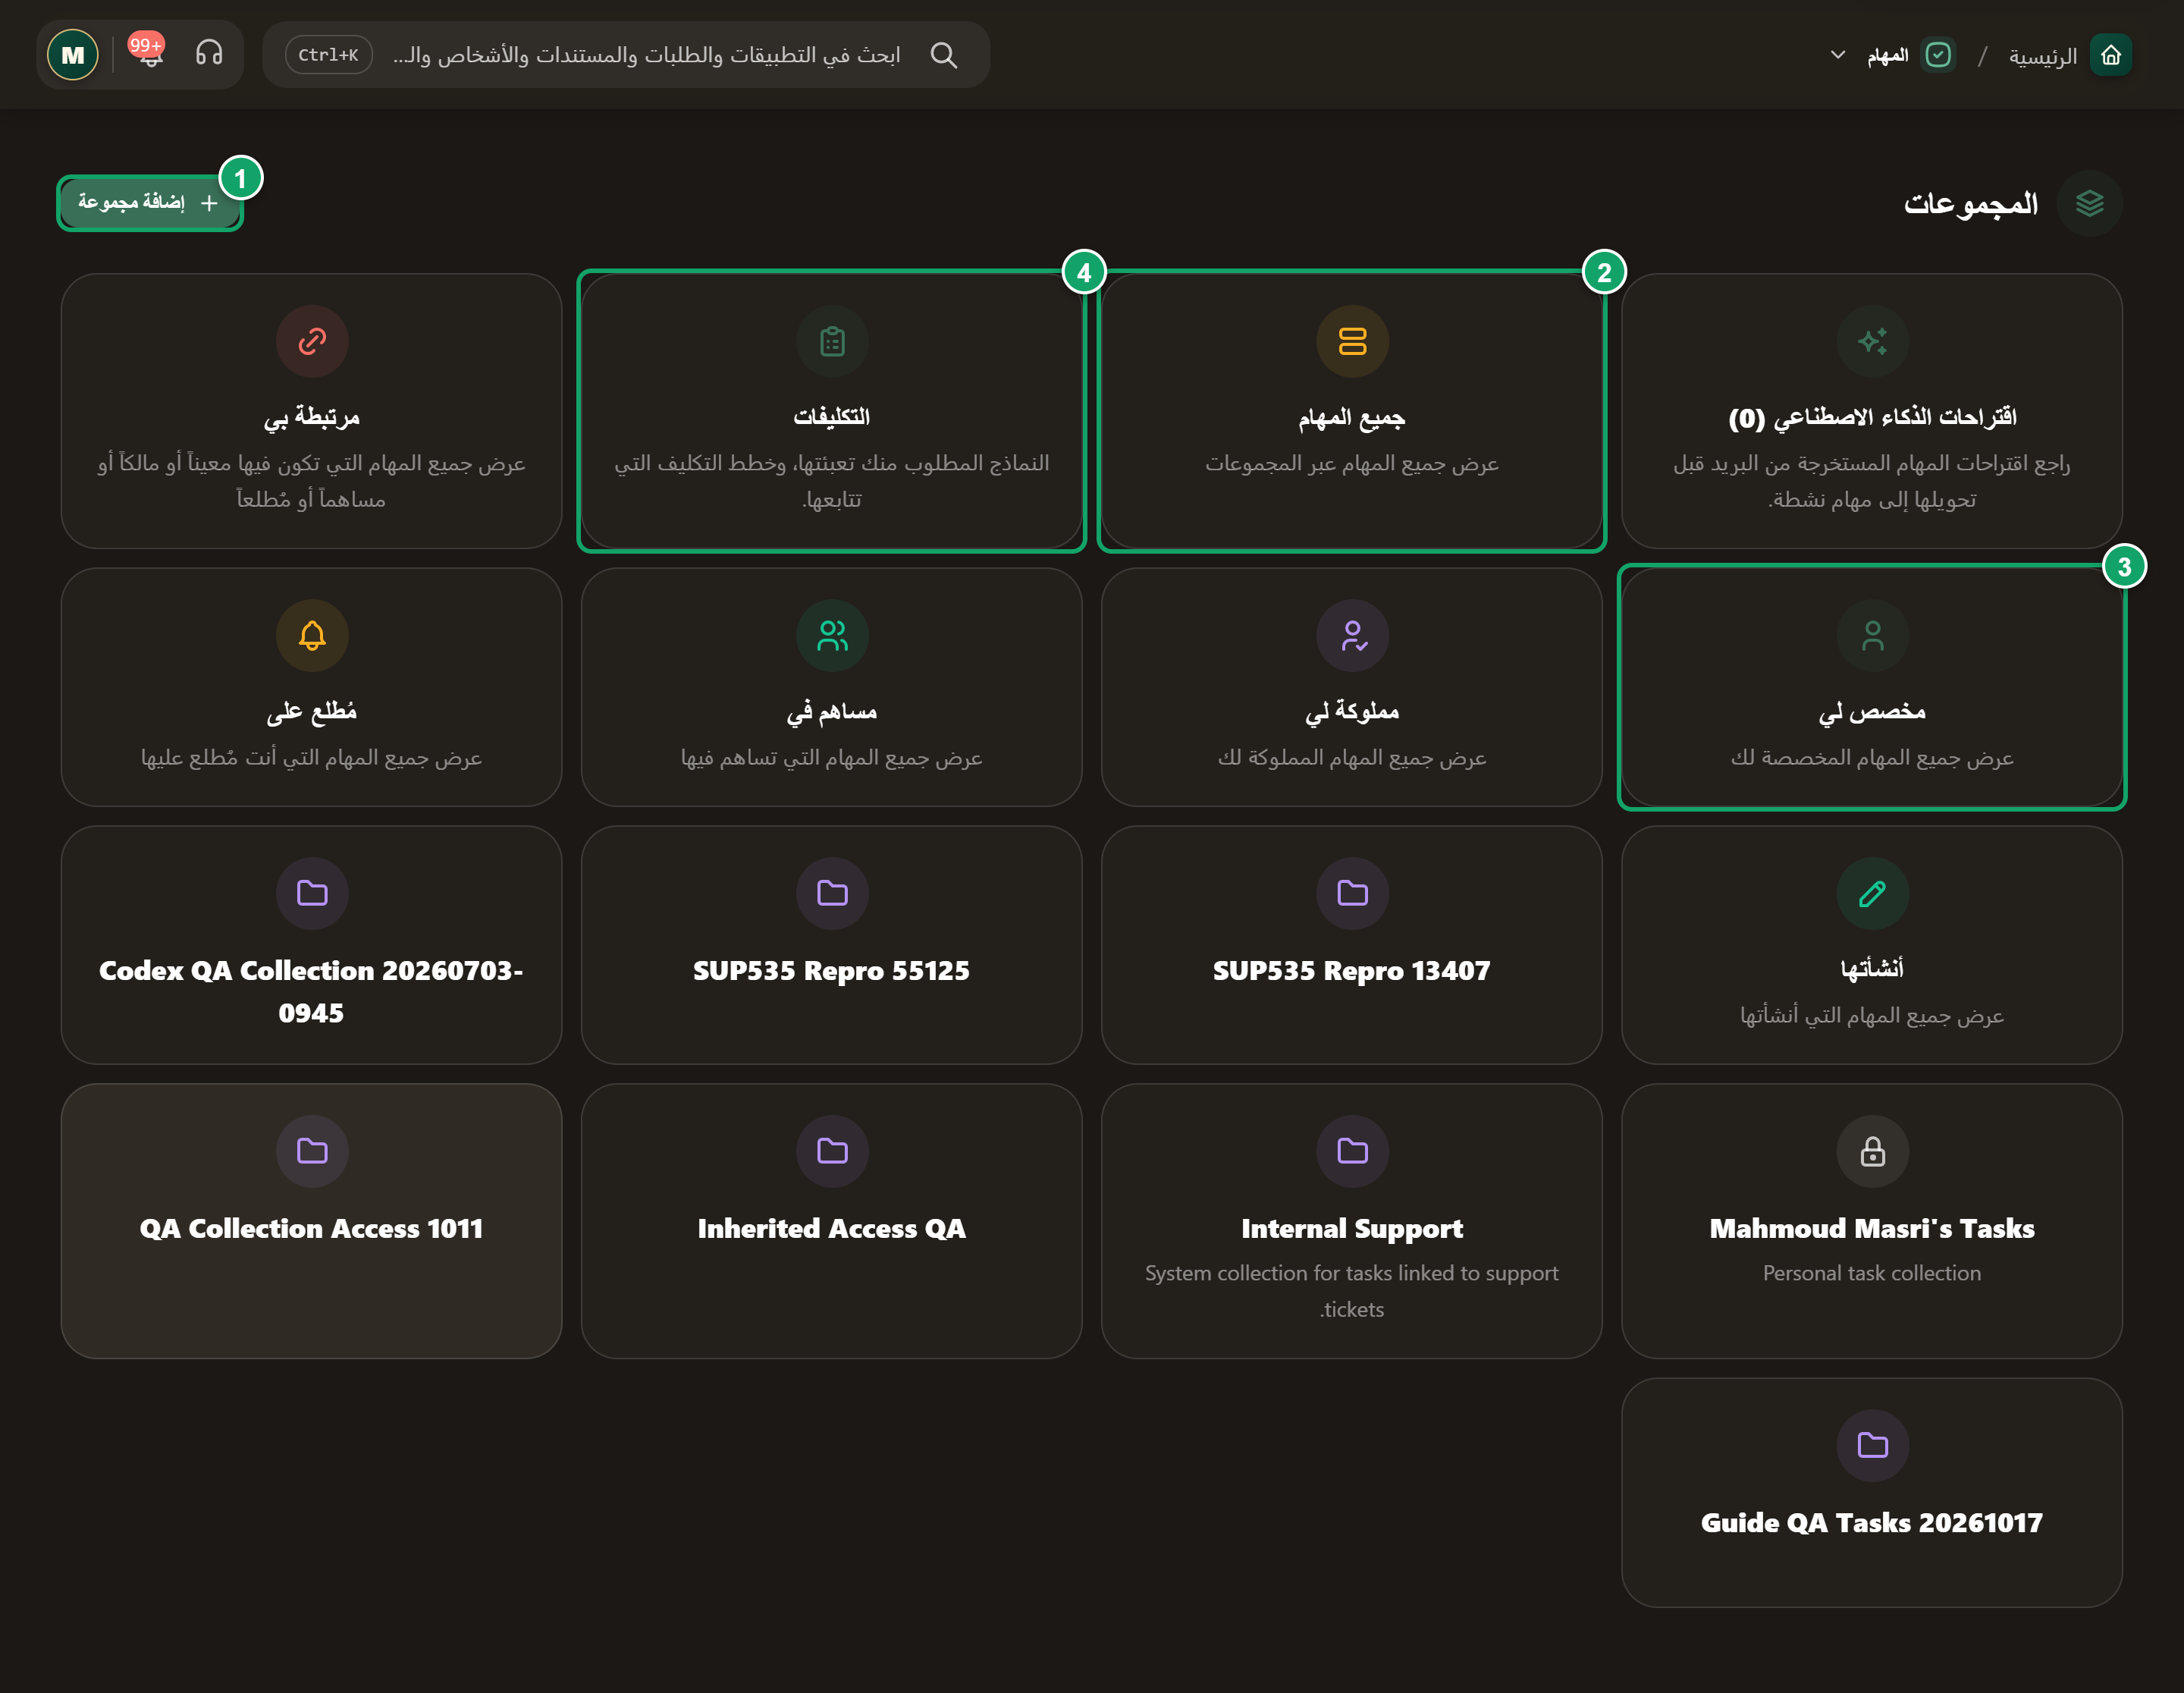
\includegraphics[width=0.95\linewidth,height=0.72\textheight,keepaspectratio]{figures/screens/ch04-collections-ar.png}
\caption{المجموعات والعروض المتاحة}
\label{fig:tasks-collections-collections}
\shotnote{تجمع صفحة «المجموعات» طريقين إلى العمل: بطاقات العروض الشخصية مثل «مخصص لي» و«التكليفات» و«اقتراحات الذكاء الاصطناعي»، ثم بطاقات المجموعات التي يمكنك الوصول إليها. لذلك ابدأ من العرض عندما تبحث عن عملك أنت، ومن المجموعة عندما تتابع عمل فريق بعينه. والمجموعات الظاهرة مجموعات اختبار في test2. ① «إضافة مجموعة». ② «جميع المهام»: يجمع كل ما يمكنك الوصول إليه. ③ «مخصص لي»: يعرض ما يجب أن تنفذه أنت. ④ «التكليفات»: تعرض النماذج المطلوب منك تعبئتها.}
\end{figure}

\begin{figure}[H]
\centering
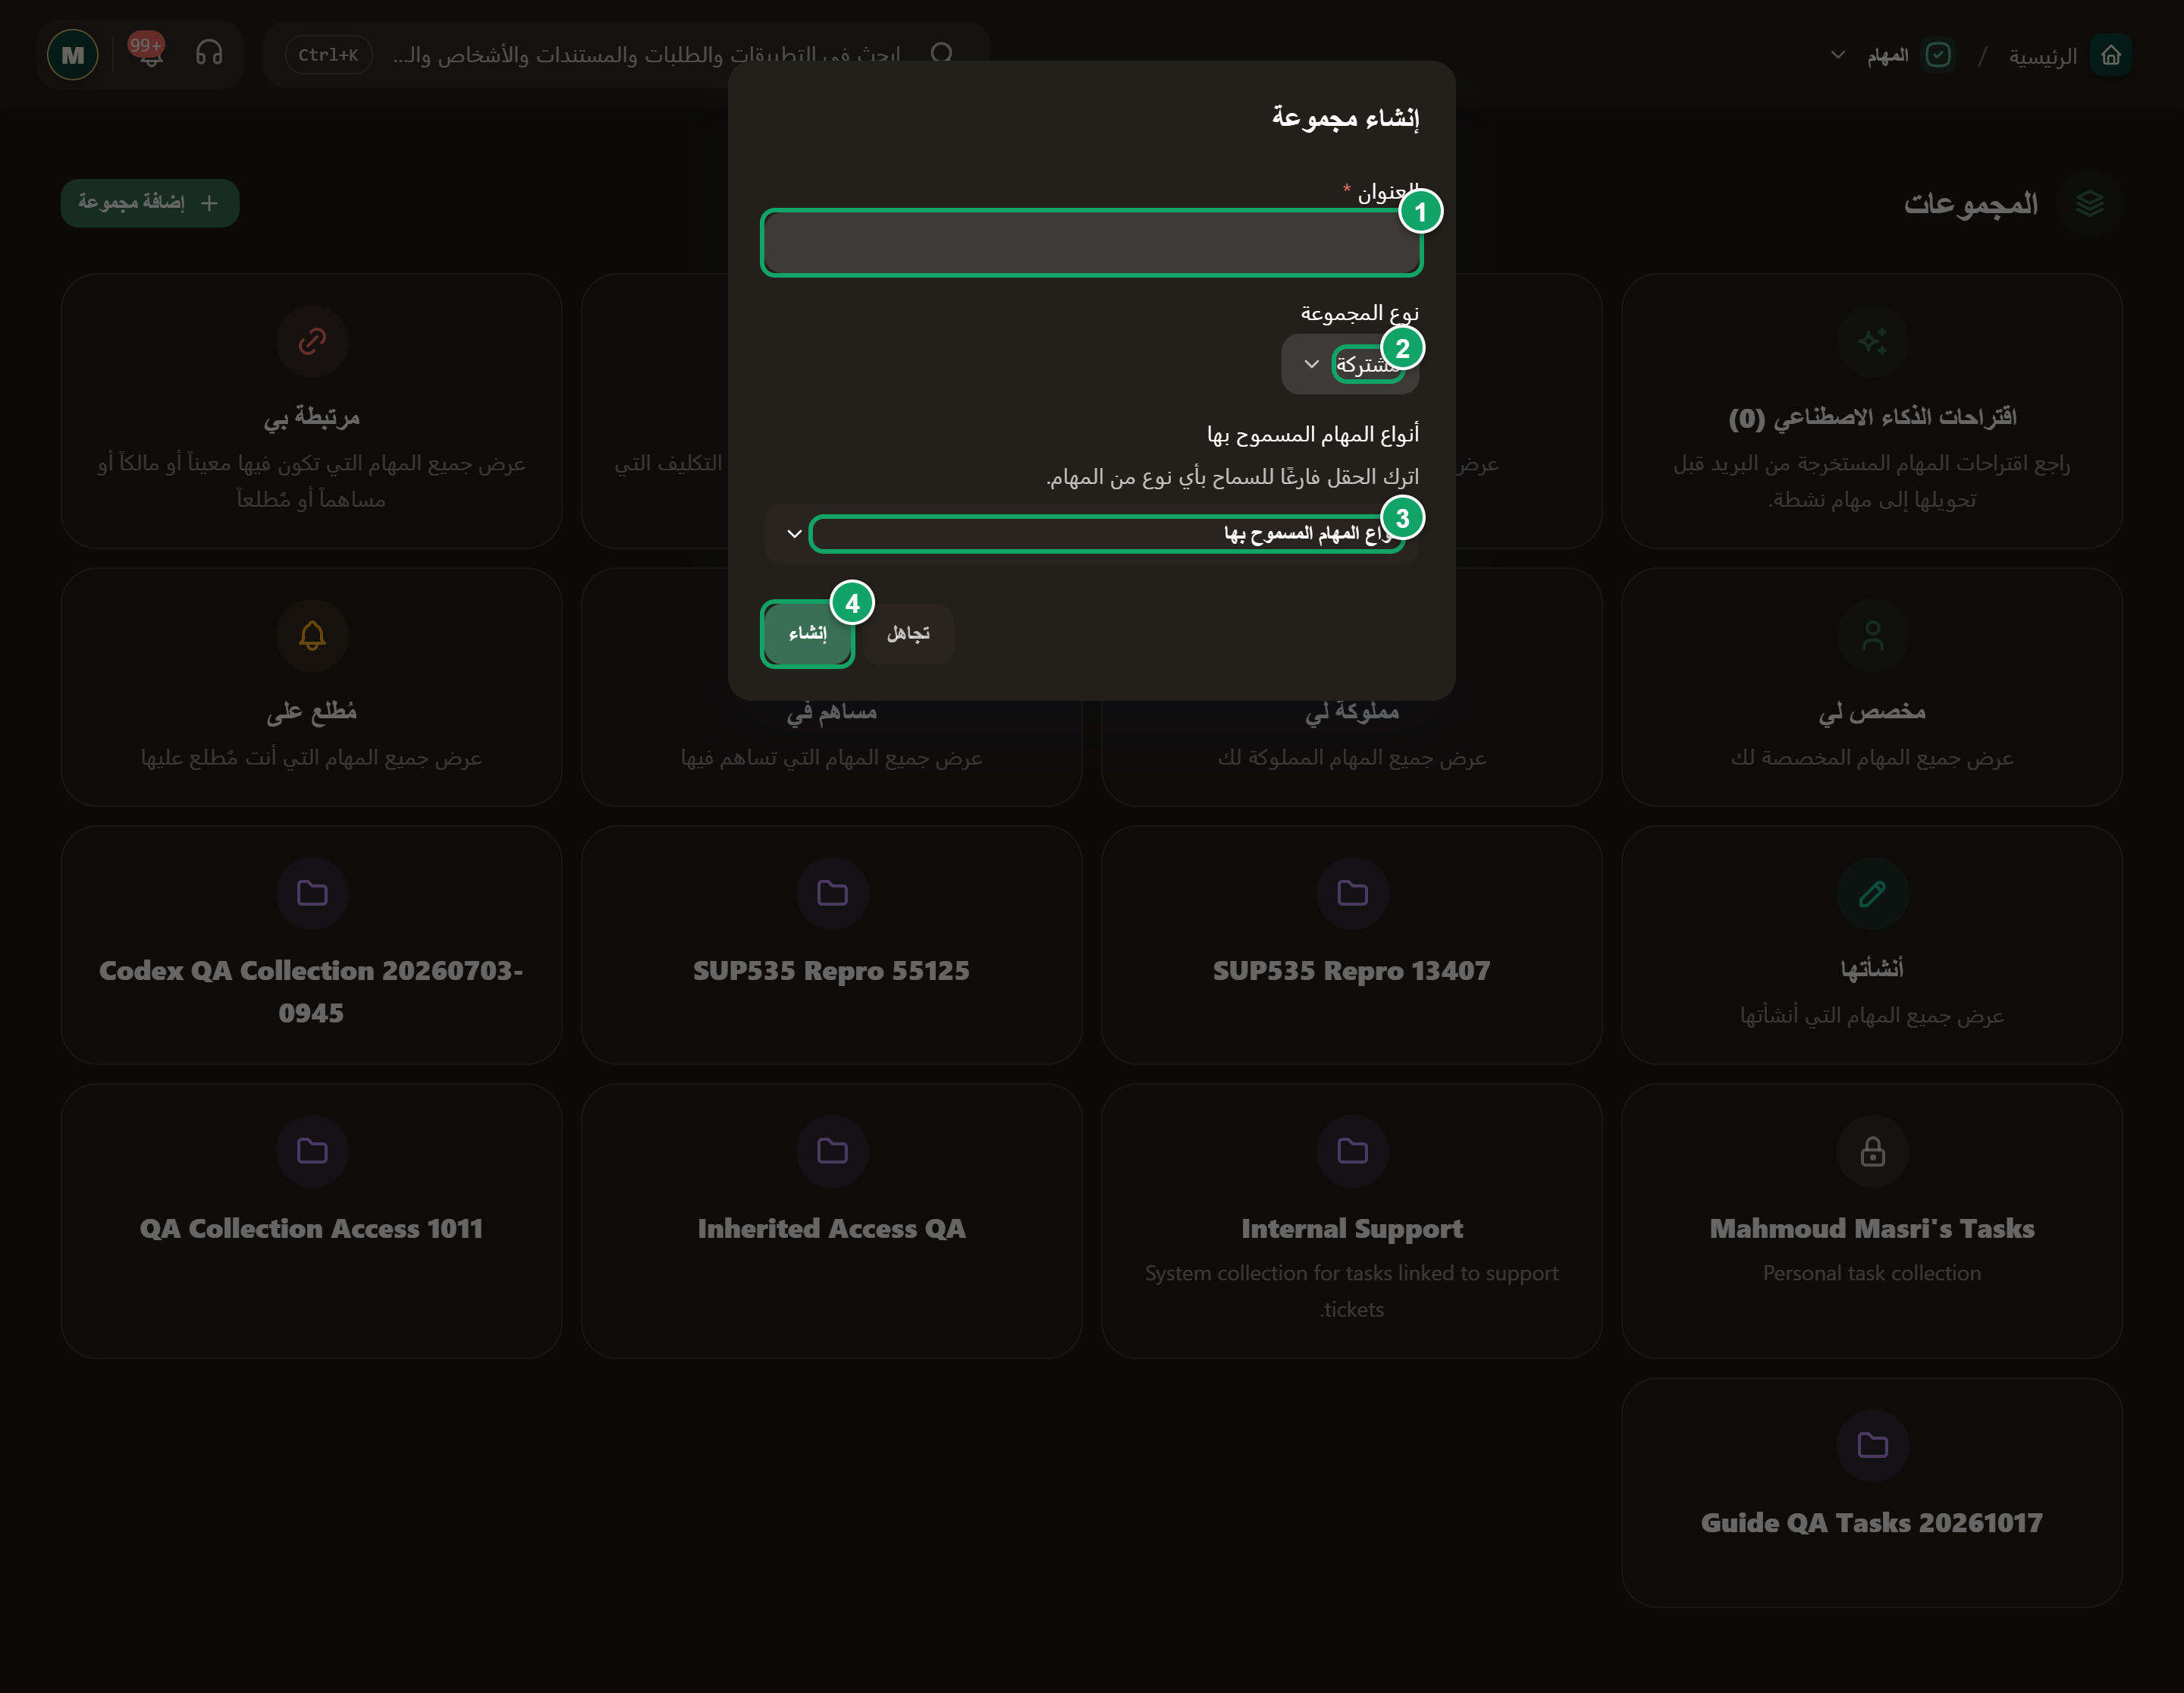
\includegraphics[width=0.95\linewidth,height=0.72\textheight,keepaspectratio]{figures/screens/ch04-collection-form-ar.png}
\caption{نموذج إنشاء مجموعة قبل الحفظ}
\label{fig:tasks-collections-collection-form}
\shotnote{يكفي لإنشاء المجموعة أن تكتب «العنوان» المطلوب وتختار «نوع المجموعة»، أي هل هي مشتركة أم شخصية. أما «أنواع المهام المسموح بها» فقيد اختياري: إذا تركته فارغاً قبلت المجموعة أي نوع متاح لك، وإذا حددت أنواعاً اقتصرت المهام فيها على تلك الأنواع. ① «العنوان» الإلزامي. ② «نوع المجموعة»: مشتركة أو شخصية. ③ «أنواع المهام المسموح بها»: قيد اختياري. ④ «إنشاء».}
\end{figure}

\begin{table}[H]
\centering
\caption{ما الذي تجده هنا؟}
\label{tab:tasks-collections-data}
\begin{tabularx}{\linewidth}{R{3.6cm} Y}
\rcHeaderRow
\thh{القسم} & \thh{المحتوى والإجراء}\\
العنوان والنوع & العنوان مطلوب، والنوع يميّز المجموعة الشخصية من المشتركة.\\
أنواع المهام المسموح بها & قيد اختياري يحدد الأنواع المقبولة داخل المجموعة، لكنه لا يمنحك صلاحية إنشاء نوع غير مسموح لك.\\
إعدادات المجموعة & تعديل البيانات والأنواع وإدارة المشاركة بحسب صلاحيتك. تأكد من وصول الفريق قبل الاعتماد على المجموعة.\\
\end{tabularx}
\end{table}

\begin{figure}[H]
\centering
\begin{tikzpicture}[node distance=0.5cm]
\node[stepBox] (a) {\RL{اختيار المجموعة}};
\node[stepBox,below=of a] (b) {\RL{مراجعة الوصول}};
\node[stepBox,below=of b] (c) {\RL{فتح مهام الفريق}};
\draw[flowsTo] (a) -- (b);
\draw[flowsTo] (b) -- (c);
\end{tikzpicture}
\rclegend
\caption{خطوات الاستخدام}
\label{fig:tasks-collections-flow}
\shotnote{يضع المخطط مراجعة الوصول بين اختيار المجموعة وتوزيع المهام فيها، لأن فتحك أنت للمجموعة لا يضمن أن الفريق يراها. فإذا وزّعت العمل في مجموعة لا يصل إليها المكلفون، لم يجدوا مهامهم فيها.}
\end{figure}

\subsection{خطوات العمل والتحقق}
\begin{enumerate}
\item ابحث أولاً عن المجموعة المطلوبة، فإن لم تجدها فاضغط «إضافة مجموعة».
\item اكتب عنواناً واضحاً، وحدد نوع المجموعة والأنواع المسموح بها عند الحاجة، ثم اضغط «إنشاء».
\item افتح المجموعة من بطاقتها، وقبل إسناد العمل تحقق من أن أعضاء الفريق المقصودين يستطيعون فتحها.
\end{enumerate}

\textbf{تحقق ومعالجة المشكلة:} يجب أن يظهر عنوان المجموعة عند فتحها. فإذا ظهرت رسالة «المجموعة غير متاحة»، فارجع إلى «المجموعات» وحدّث الصفحة، ثم اطلب مراجعة المشاركة والصلاحيات، ولا تنشئ نسخاً مكررة من المجموعة.

\clearpage
\section{عروض المهام}
\label{sec:tasks-feature-views}

يغيّر العرض طريقة العثور على المهام ومتابعتها دون أن يغيّر المهام نفسها. استخدم «قائمة» لمراجعة التفاصيل، و«لوحة» لتوزيع العمل حسب الحالة، و«المتابعة اليومية» لمراجعة تحديثات الفريق.

\textbf{المسار ومن يستخدمه:} «المهام» ← مجموعة أو أحد عروضك الشخصية. يستخدمها الموظف والمدير يومياً.

\begin{rcnote}[مثال: شركة الأفق]
يفتح عمر «مخصص لي» ليعرف العمل المطلوب منه، وتراجع سارة لوحة «زيارات الأفق» لترى المهام التي لم تبدأ بعد.
\end{rcnote}

\begin{figure}[H]
\centering
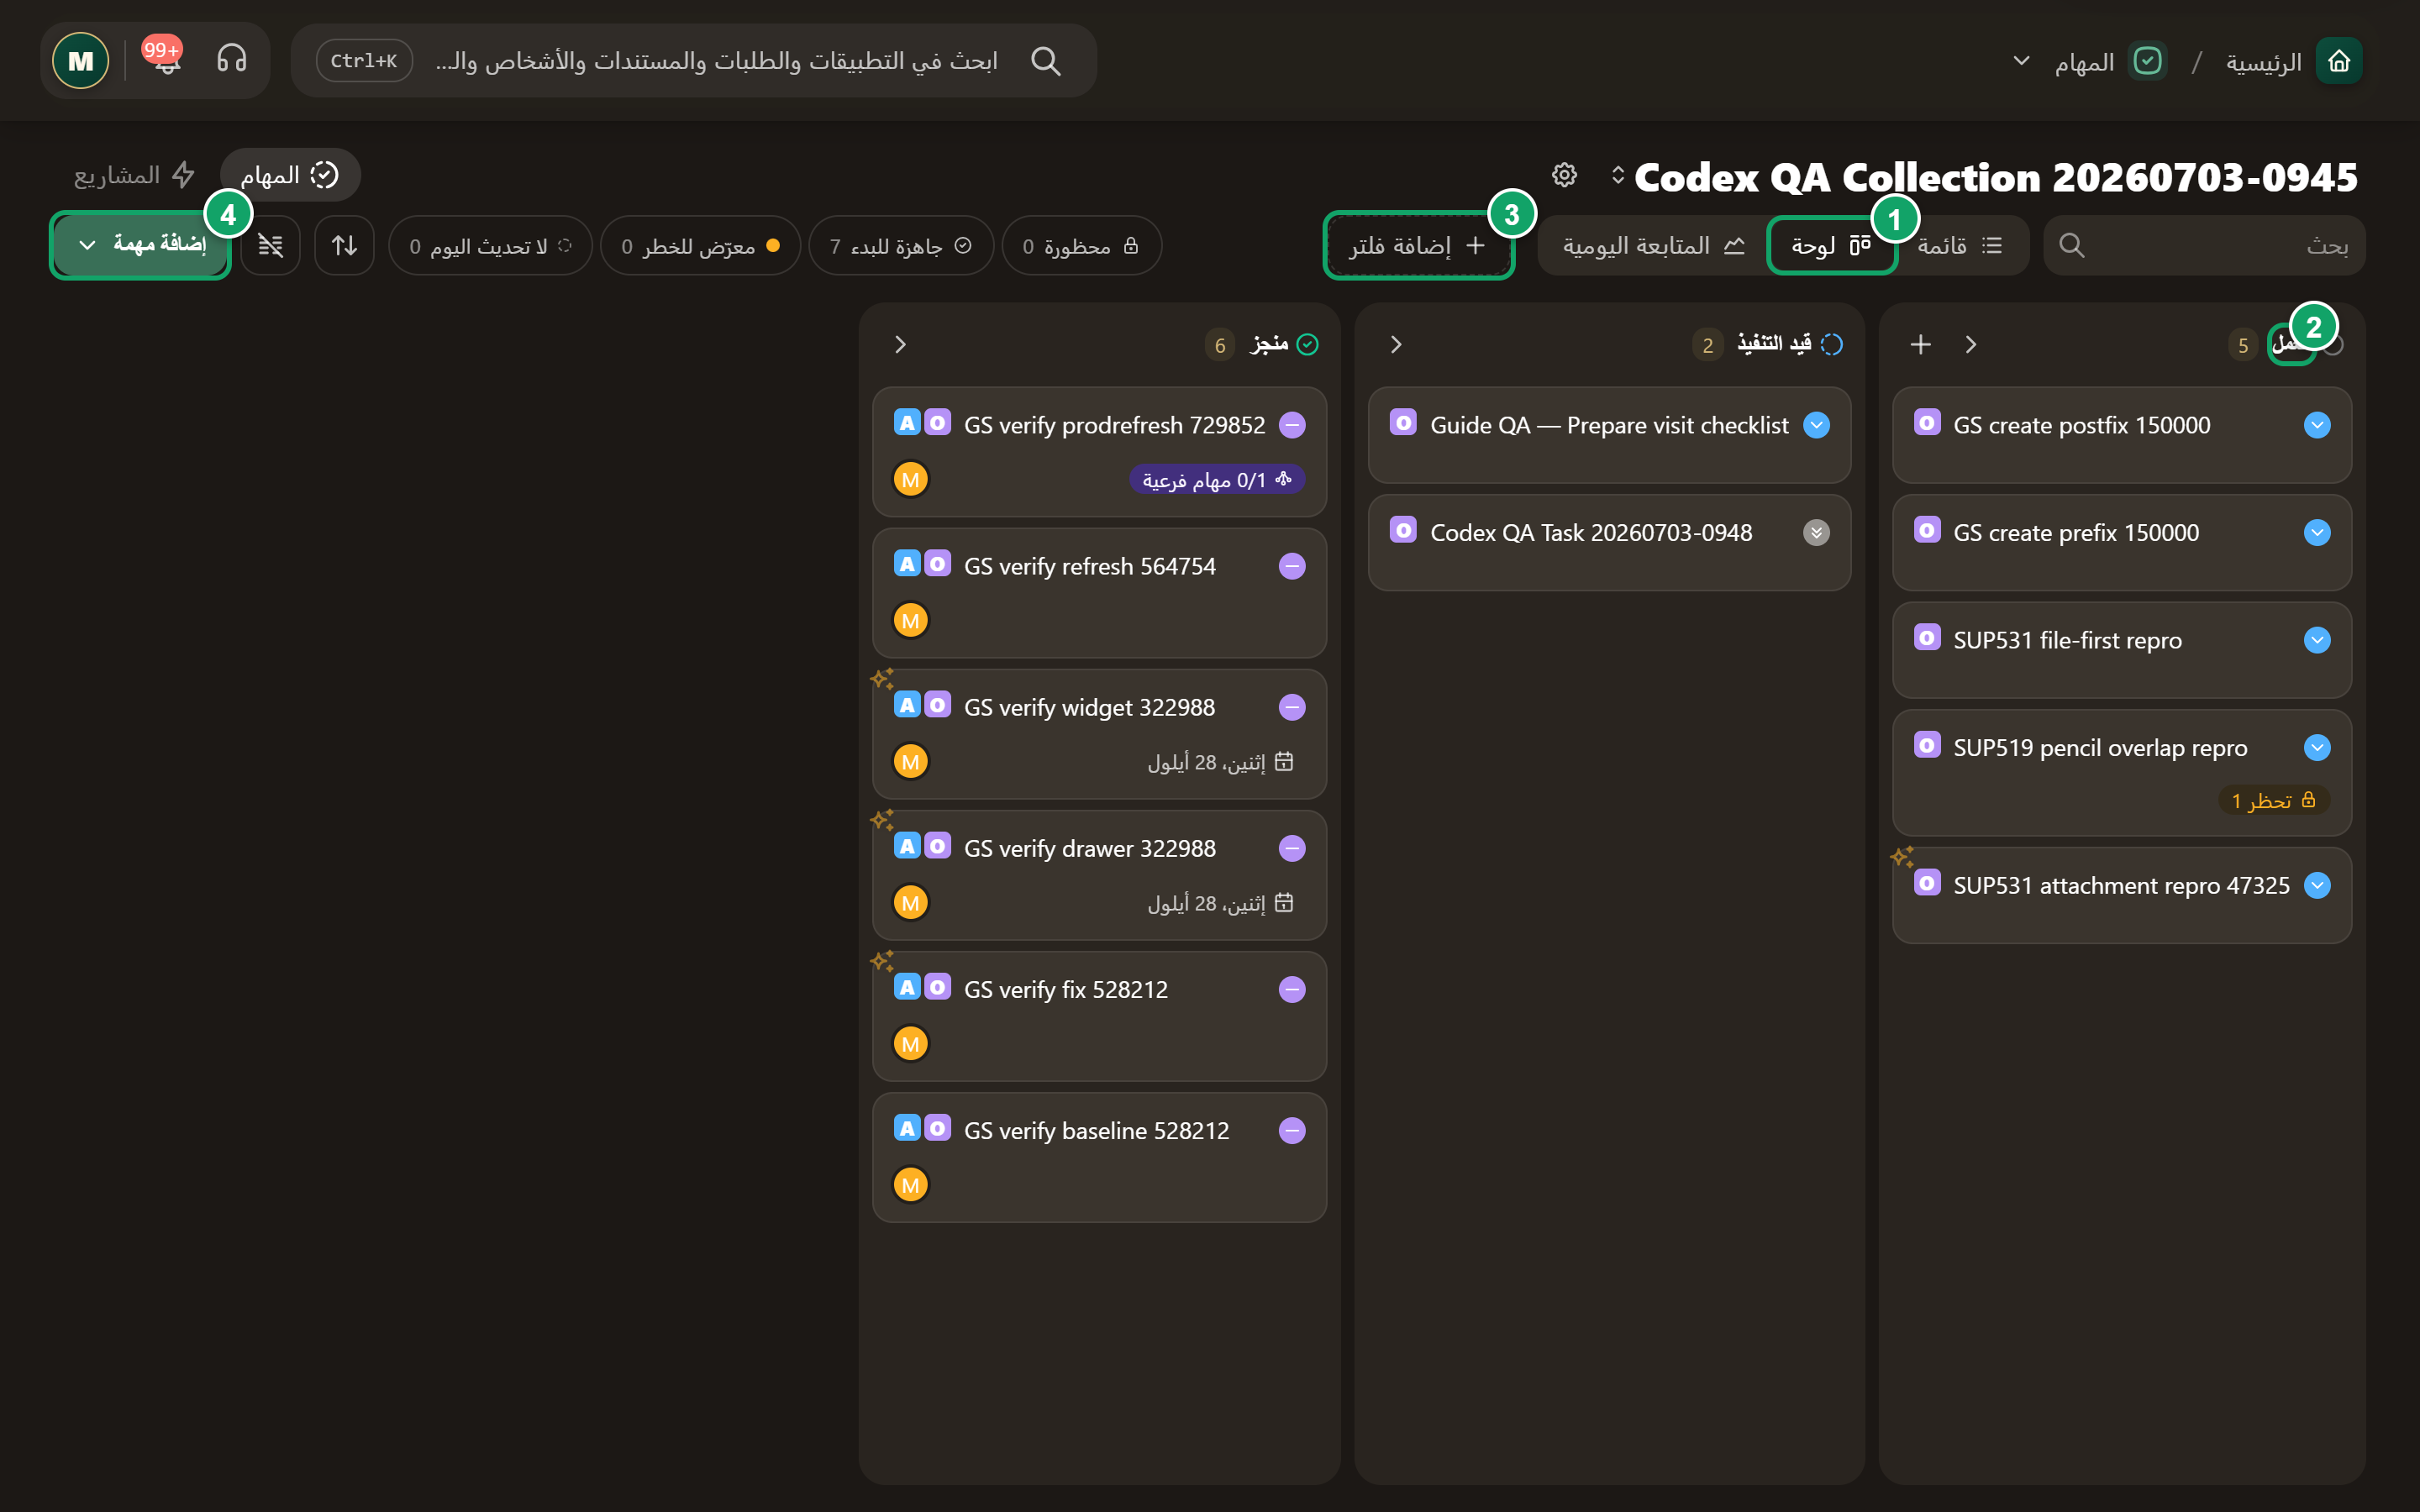
\includegraphics[width=0.95\linewidth,height=0.72\textheight,keepaspectratio]{figures/screens/ch04-board-ar.png}
\caption{لوحة مجموعة اختبار}
\label{fig:tasks-views-board}
\shotnote{تعرض «لوحة» مهام المجموعة في أعمدة تمثل الحالات، مثل «للعمل» و«قيد التنفيذ» و«منجز»، فترى في نظرة واحدة أين يقف العمل وأين يتراكم. وتعرض الشارات مثل «محظورة» و«جاهزة للبدء» عدد المهام التي تحتاج انتباهك. ولا تعني رؤيتك للمهمة أنك تستطيع تعديلها أو نقلها. ① «لوحة». ② عمود «للعمل» وفيه المهام التي لم تبدأ. ③ «إضافة فلتر». ④ «إضافة مهمة».}
\end{figure}

\begin{figure}[H]
\centering
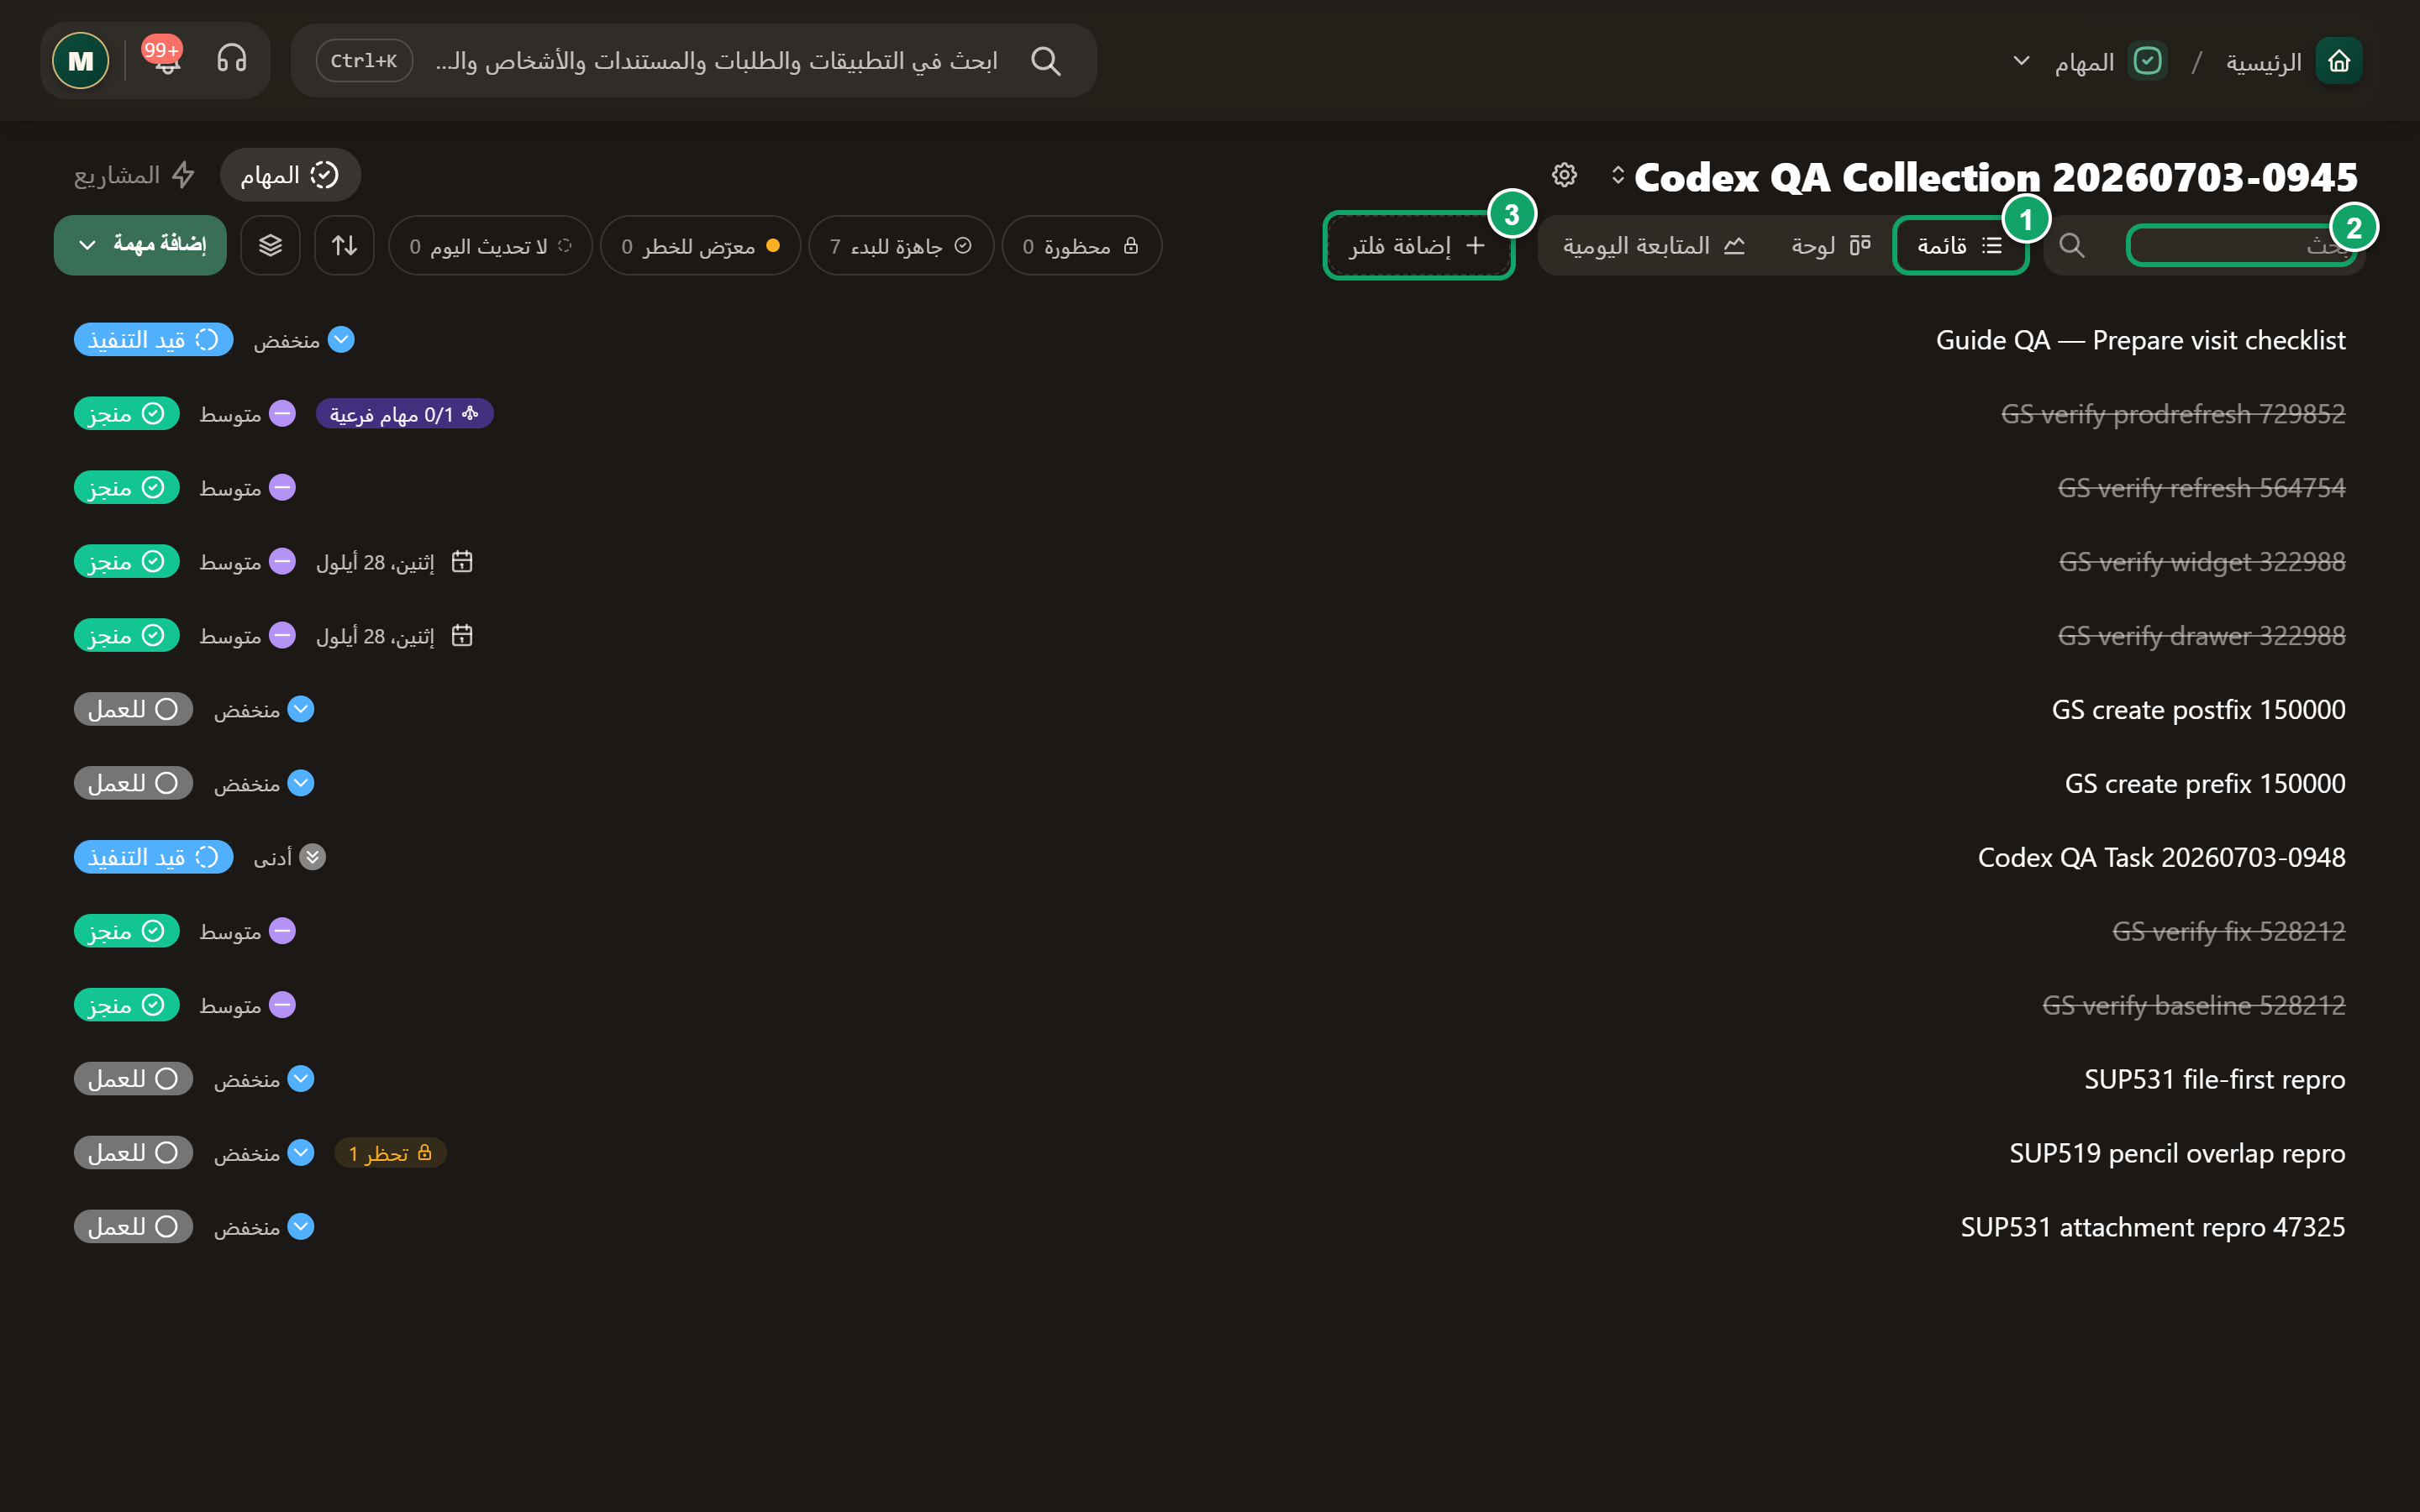
\includegraphics[width=0.95\linewidth,height=0.72\textheight,keepaspectratio]{figures/screens/ch04-list-ar.png}
\caption{عرض القائمة}
\label{fig:tasks-views-list}
\shotnote{يعرض «قائمة» المهام نفسها في صفوف تبيّن حالة كل مهمة وأولويتها وموعدها، وتظهر المهام المنجزة بخط مشطوب. لذلك يناسب هذا العرض مقارنة المهام ومراجعة تفاصيلها، ويساعدك البحث و«إضافة فلتر» والترتيب على تضييق النتائج عندما تكثر المهام. ① «قائمة». ② مربع «بحث» للعثور على المهمة بعنوانها. ③ «إضافة فلتر».}
\end{figure}

\begin{figure}[H]
\centering
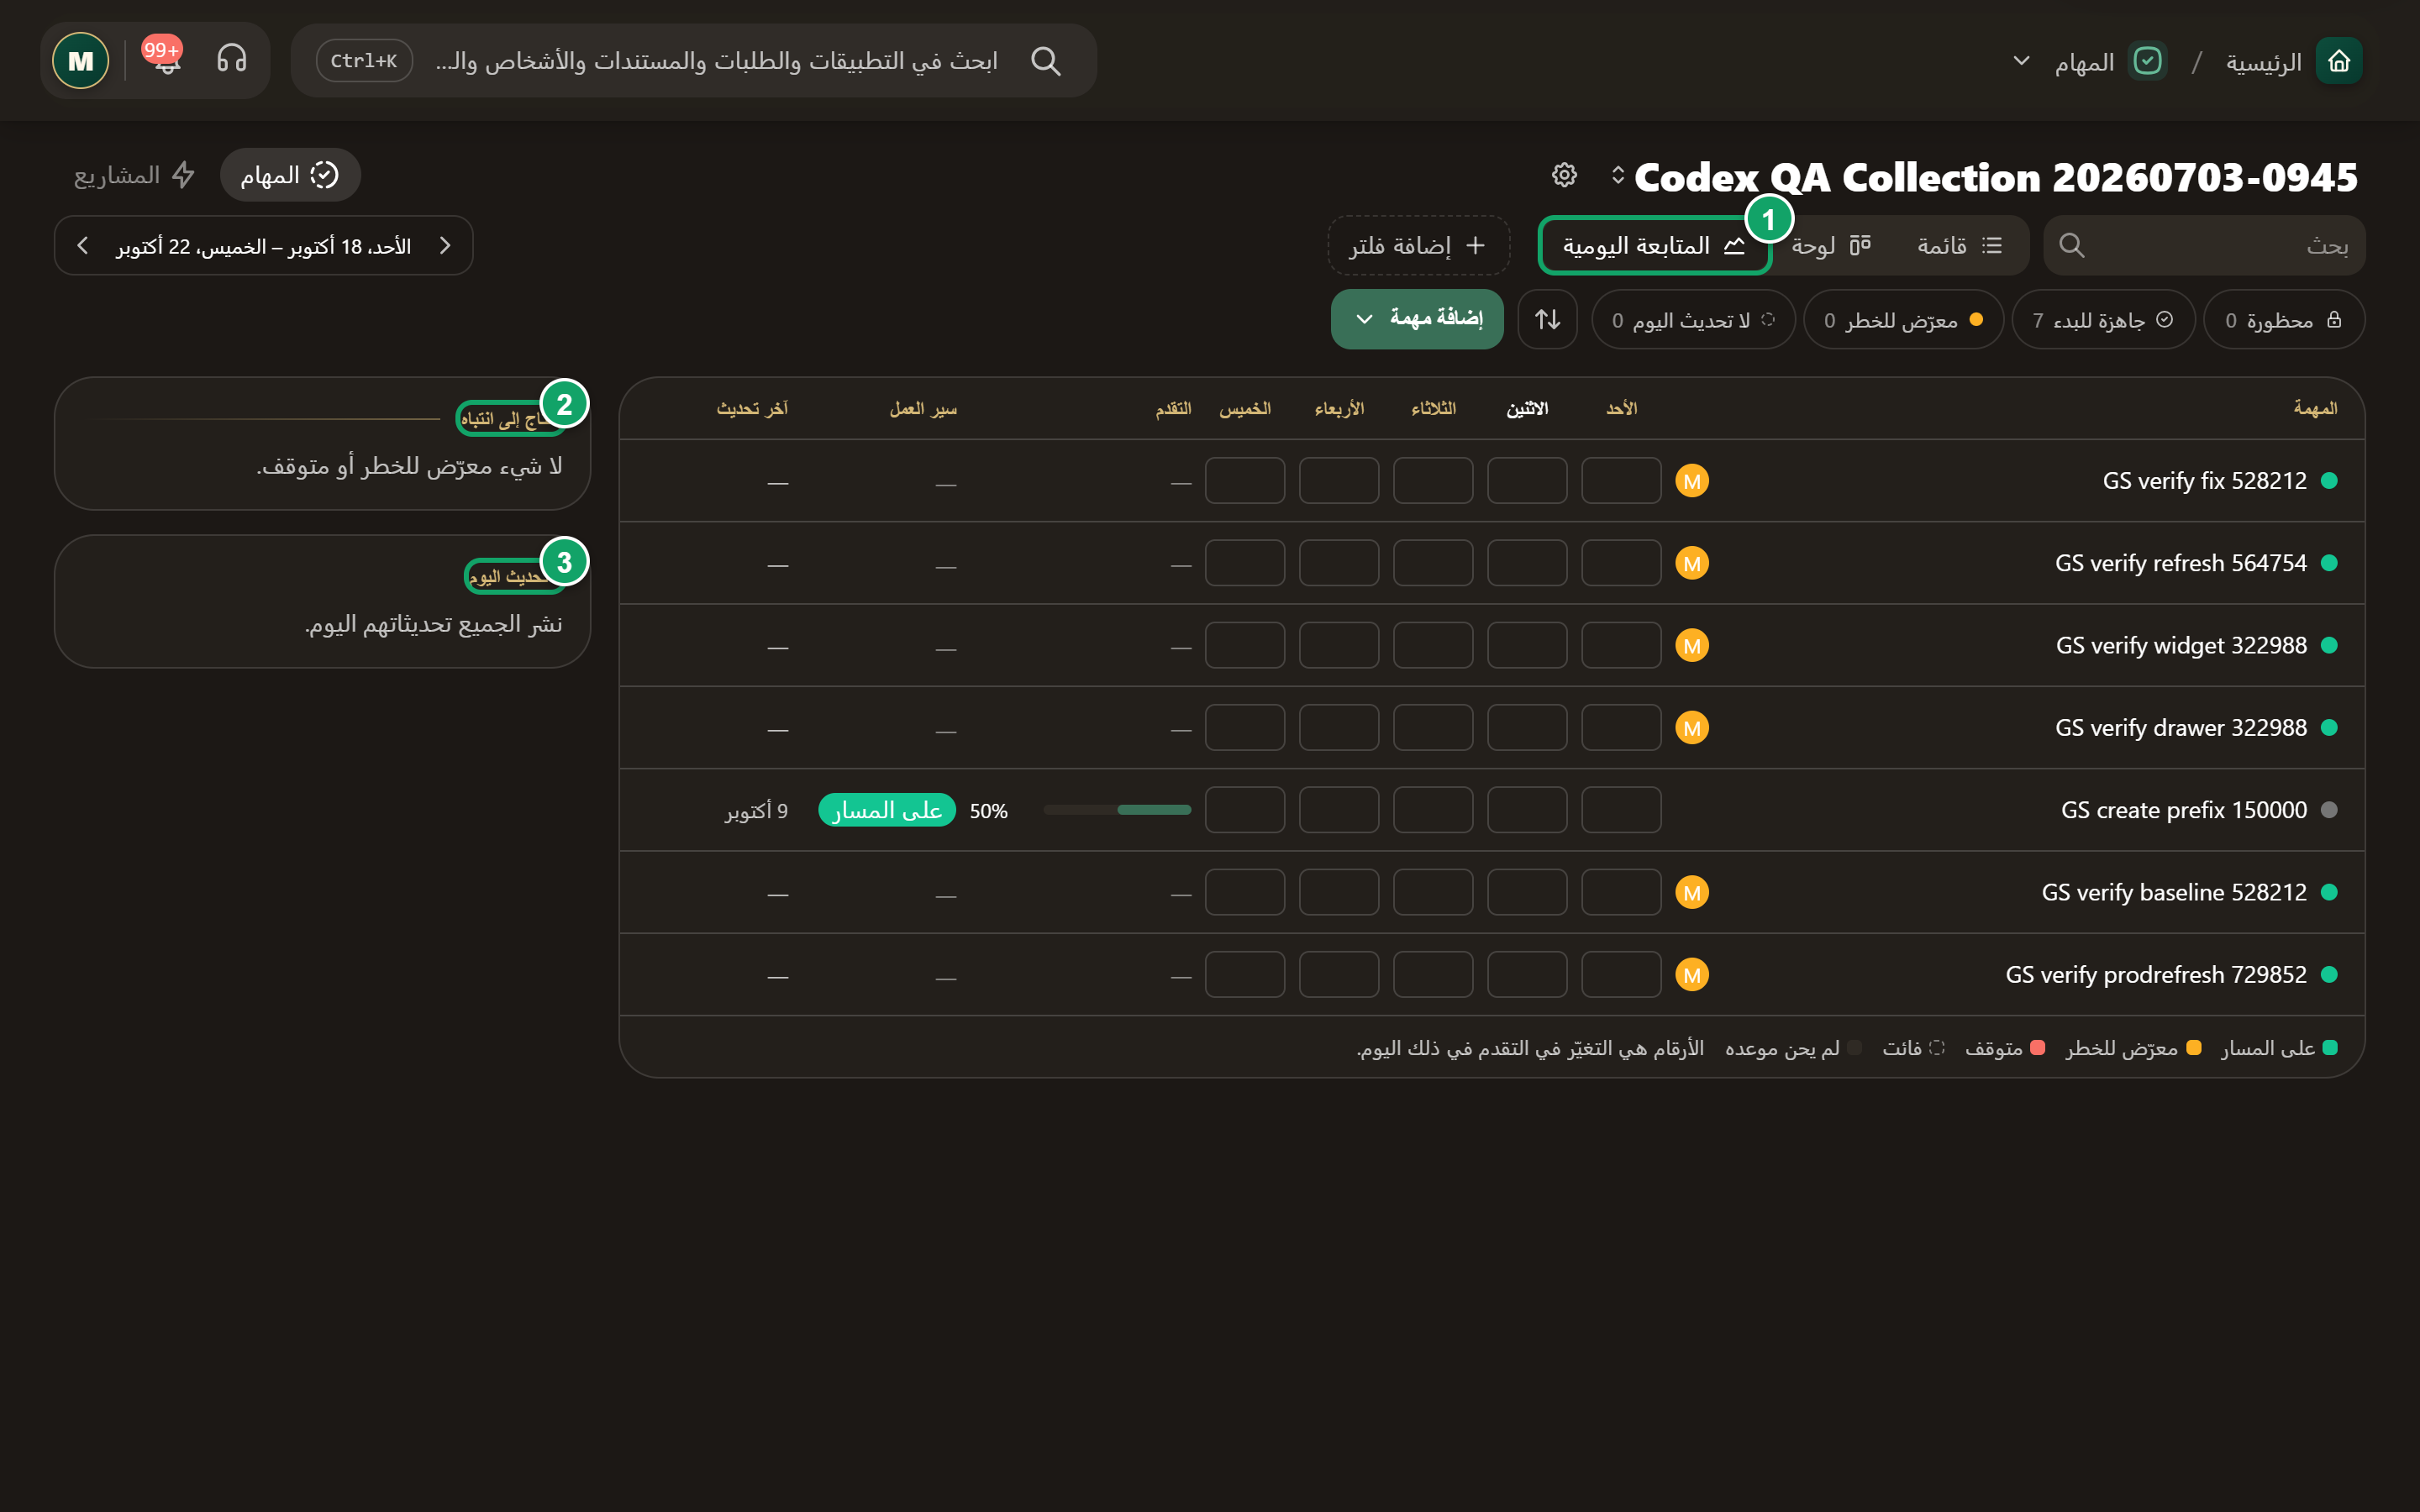
\includegraphics[width=0.95\linewidth,height=0.72\textheight,keepaspectratio]{figures/screens/ch04-checkins-ar.png}
\caption{عرض المتابعة اليومية}
\label{fig:tasks-views-checkins}
\shotnote{يعرض «المتابعة اليومية» تحديثات كل مهمة على أيام الأسبوع المحدد، مع التقدم و«سير العمل» و«آخر تحديث». وتجمع بطاقتا «يحتاج إلى انتباه» و«لا تحديث اليوم» ما يستدعي المتابعة. ولا يعني غياب التحديث أن المهمة اكتملت، بل أن أحداً لم ينشر عنها تحديثاً. ① «المتابعة اليومية». ② «يحتاج إلى انتباه»: المهام المعرضة للخطر أو المحظورة. ③ «لا تحديث اليوم».}
\end{figure}

\begin{table}[H]
\centering
\caption{ما الذي تجده هنا؟}
\label{tab:tasks-views-data}
\begin{tabularx}{\linewidth}{R{3.6cm} Y}
\rcHeaderRow
\thh{القسم} & \thh{المحتوى والإجراء}\\
جميع المهام؛ مرتبطة بي & الأول يجمع كل ما يمكنك الوصول إليه، والثاني يقتصر على المهام التي لك فيها دور.\\
مخصص لي؛ مملوكة لي & الأول يعرض التنفيذ المطلوب منك، والثاني يعرض المهام التي تتحمل مسؤولية نتيجتها.\\
مساهم في؛ مُطلع على؛ أنشأتها & عروض منفصلة للمهام التي تساهم فيها، والتي تتابعها للاطلاع، والتي أنشأتها.\\
البحث والتصفية والعرض & ابحث بالعنوان، ثم صفِّ النتائج ورتّبها وجمّعها بالخيارات المعروضة. أما إجراءات اللوحة الجماعية فتخضع لصلاحيات المهام وانتقالات حالاتها.\\
\end{tabularx}
\end{table}

\begin{figure}[H]
\centering
\begin{tikzpicture}[node distance=0.5cm]
\node[stepBox] (a) {\RL{اختيار دور أو مجموعة}};
\node[stepBox,below=of a] (b) {\RL{بحث وتصفية}};
\node[stepBox,below=of b] (c) {\RL{فتح المهمة}};
\draw[flowsTo] (a) -- (b);
\draw[flowsTo] (b) -- (c);
\end{tikzpicture}
\rclegend
\caption{خطوات الاستخدام}
\label{fig:tasks-views-flow}
\shotnote{يبيّن المخطط ترتيب البحث: ابدأ بالعرض الذي يطابق دورك أو بالمجموعة التي تتابعها، ثم ضيّق النتائج، وبعدها افتح المهمة. فإذا بدأت من عرض لا يخصك، فقد تظن أن المهمة مفقودة وهي في عرض آخر.}
\end{figure}

\subsection{خطوات العمل والتحقق}
\begin{enumerate}
\item افتح المجموعة أو العرض المناسب لدورك، ثم ابحث عن عنوان المهمة.
\item انتقل بين «قائمة» و«لوحة»، وراجع التصفية قبل أن تستنتج أن المهمة مفقودة.
\item افتح المهمة من بطاقتها، وإذا ظهرت قائمة إجراءات فاختر «فتح». ثم راجع حالتها والمسؤول عنها.
\end{enumerate}

\textbf{تحقق ومعالجة المشكلة:} إذا لم تجد المهمة، فأزل التصفية وراجع المجموعة ودورك وصلاحية الوصول. وتذكّر أن تغيير العرض لا يغيّر حالة العمل.

\clearpage
\section{إنشاء المهمة وتفاصيلها}
\label{sec:tasks-feature-details}

تسجّل المهمة نتيجة مطلوبة ومن يتولاها. اكتب عنواناً محدداً، ثم حدد المسؤولية والموعد والمعلومات اللازمة للتنفيذ.

\textbf{المسار ومن يستخدمه:} «المهام» ← مجموعة ← «إضافة مهمة». يستخدمها من يوزّع العمل ومن ينفّذه.

\begin{rcnote}[مثال: شركة الأفق]
تنشئ سارة مهمة «تجهيز قائمة الزيارة» في مجموعة «زيارات الأفق» وتسندها إلى عمر قبل موعد الزيارة، بينما تبقى هي المسؤولة عن النتيجة.
\end{rcnote}

\begin{figure}[H]
\centering
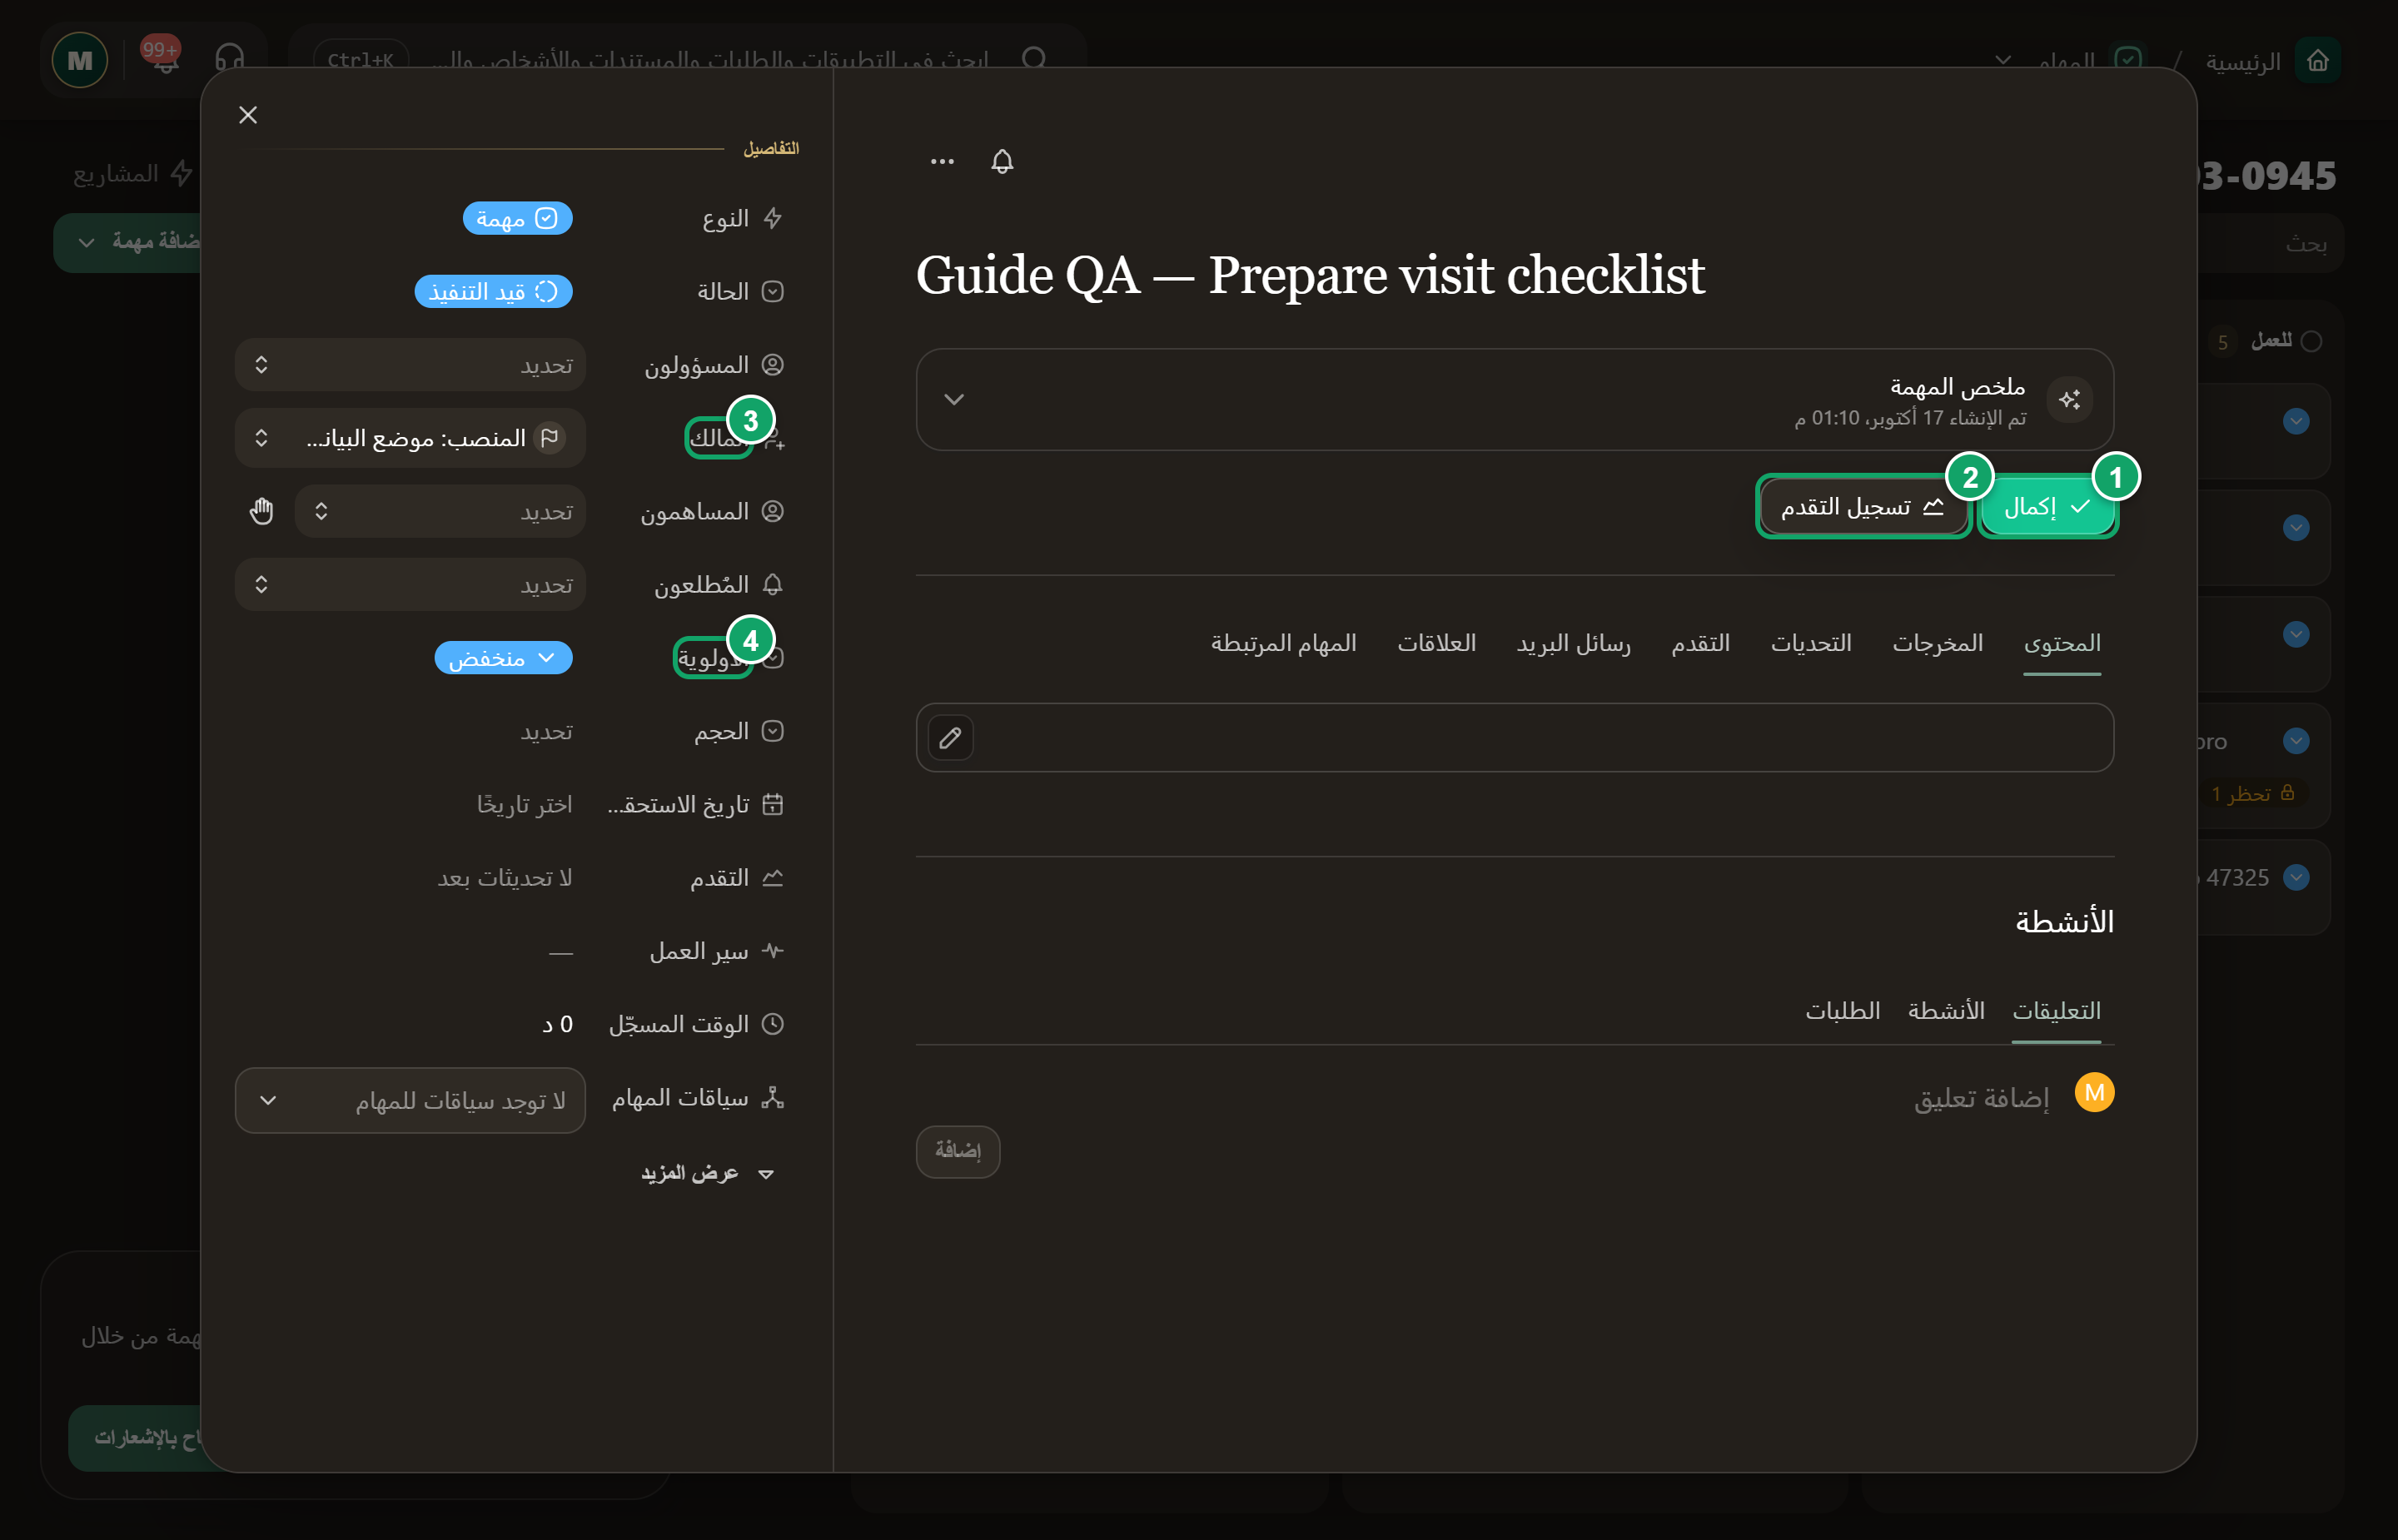
\includegraphics[width=0.95\linewidth,height=0.72\textheight,keepaspectratio]{figures/screens/ch04-details-ar.png}
\caption{تفاصيل مهمة اختبار محفوظة}
\label{fig:tasks-details-details}
\shotnote{تجمع لوحة «التفاصيل» ما يحدد المسؤولية والتخطيط: من ينفّذ، ومن يملك النتيجة، ومن يساهم أو يطّلع، ثم الأولوية والموعد. ويكشف «عرض المزيد» الفئة والمجموعات والمنشئ وتاريخ الإنشاء، ويملأ النظام الأخيرين بنفسه. ولاحظ أن «المالك» قد يكون منصباً لا شخصاً؛ والمهمة الظاهرة مهمة اختبار في test2. ① زر الإجراء الرئيسي، مثل «ابدأ» أو «إكمال». ② «تسجيل التقدم»: ينشر تحديثاً عن العمل. ③ «المالك»: المسؤول عن النتيجة. ④ «الأولوية».}
\end{figure}

\begin{table}[H]
\centering
\caption{ما الذي تجده هنا؟}
\label{tab:tasks-details-data}
\begin{tabularx}{\linewidth}{R{3.6cm} Y}
\rcHeaderRow
\thh{القسم} & \thh{المحتوى والإجراء}\\
العنوان والنوع والحالة & يوضح العنوان النتيجة المطلوبة، ويحدد النوع الإعدادات والقواعد، وتعكس الحالة مرحلة العمل.\\
الأشخاص & يتولى «المسؤولون» التنفيذ، ويُسأل «المالك» عن النتيجة، ويقدّم «المساهمون» جزءاً من العمل، ويحتاج «المطّلعون» إلى المتابعة فقط. وقد تعرض الخيارات أعضاء أو مناصب بحسب الإعداد.\\
التخطيط & الأولوية والحجم وتاريخ الاستحقاق وسياقات المهام. اختر ما يخدم المهمة، فليست كل الروابط إلزامية.\\
عرض المزيد & الفئة و«المشاريع» (المهام الكبرى) والوسوم والمجموعات، إضافة إلى المنشئ وتاريخ الإنشاء اللذين يملؤهما النظام.\\
المحتوى & الوصف والمخرجات والتحديات، ثم التقدم والبريد والعلاقات عند توفرها. وتشرحها الصفحتان التاليتان.\\
المشاركة والحذف & تتيح قائمة المزيد المشاركة عند السماح بها، أو الحذف بعد التأكيد. أكمل المهمة إذا أردت الاحتفاظ بسجل العمل المنجز، لأن الحذف يزيلها.\\
\end{tabularx}
\end{table}

\begin{figure}[H]
\centering
\begin{tikzpicture}[node distance=0.5cm]
\node[stepBox] (a) {\RL{نتيجة واضحة}};
\node[stepBox,below=of a] (b) {\RL{مسؤولية وموعد}};
\node[stepBox,below=of b] (c) {\RL{إنشاء ثم تحقق}};
\draw[flowsTo] (a) -- (b);
\draw[flowsTo] (b) -- (c);
\end{tikzpicture}
\rclegend
\caption{خطوات الاستخدام}
\label{fig:tasks-details-flow}
\shotnote{يرتب المخطط إنشاء المهمة في ثلاث خطوات: صياغة النتيجة المطلوبة، ثم تحديد من يتولاها ومتى، ثم الإنشاء والتحقق. فالعنوان الواضح يسهّل اختيار المسؤول المناسب، وإعادة فتح المهمة بعد إنشائها تؤكد أن بياناتها حُفظت كما أردت.}
\end{figure}

\subsection{خطوات العمل والتحقق}
\begin{enumerate}
\item اختر «إضافة مهمة» ثم النوع المتاح. اكتب عنواناً يصف النتيجة، وأضف الوصف.
\item حدد المسؤولين عن التنفيذ والمالك، والموعد والأولوية عند الحاجة، وراجع العلاقات المطلوبة قبل الإنشاء.
\item اضغط «إنشاء»، ثم افتح المهمة من القائمة أو اللوحة وتحقق من العنوان والمسؤولية والحالة.
\item بعد تعديل أي حقل في المهمة المحفوظة، انتظر تأكيد الحفظ. أما في محرر النص فاستخدم إجراء الحفظ، ثم أعد فتح المهمة للتأكد.
\end{enumerate}

\textbf{تحقق ومعالجة المشكلة:} إذا تعذّر الحفظ، فراجع رسالة الخطأ والنوع والعلاقات المطلوبة وصلاحيتك. ولا تفترض أن النص حُفظ لمجرد إغلاق النافذة.

\clearpage
\section{التقدم والنتائج والتواصل}
\label{sec:tasks-feature-follow-up}

تجمع المهمة ما أُنجز وما يعيق العمل وما يحتاجه أفراد الفريق بعضهم من بعض. حدّث النتيجة والحالة باستمرار حتى يتابع زميلك العمل دون تخمين.

\textbf{المسار ومن يستخدمه:} افتح مهمة محفوظة، واستخدم تبويبات المحتوى وقسم «الأنشطة». يستخدمها المنفّذ والمساهم والمسؤول عن النتيجة.

\begin{rcnote}[مثال: شركة الأفق]
يسجّل عمر ما أعدّه لقائمة الزيارة، ويوضح أن عنوان الموقع لم يصل بعد، فتراجع سارة العائق وتحدد الخطوة التالية.
\end{rcnote}

\begin{figure}[H]
\centering
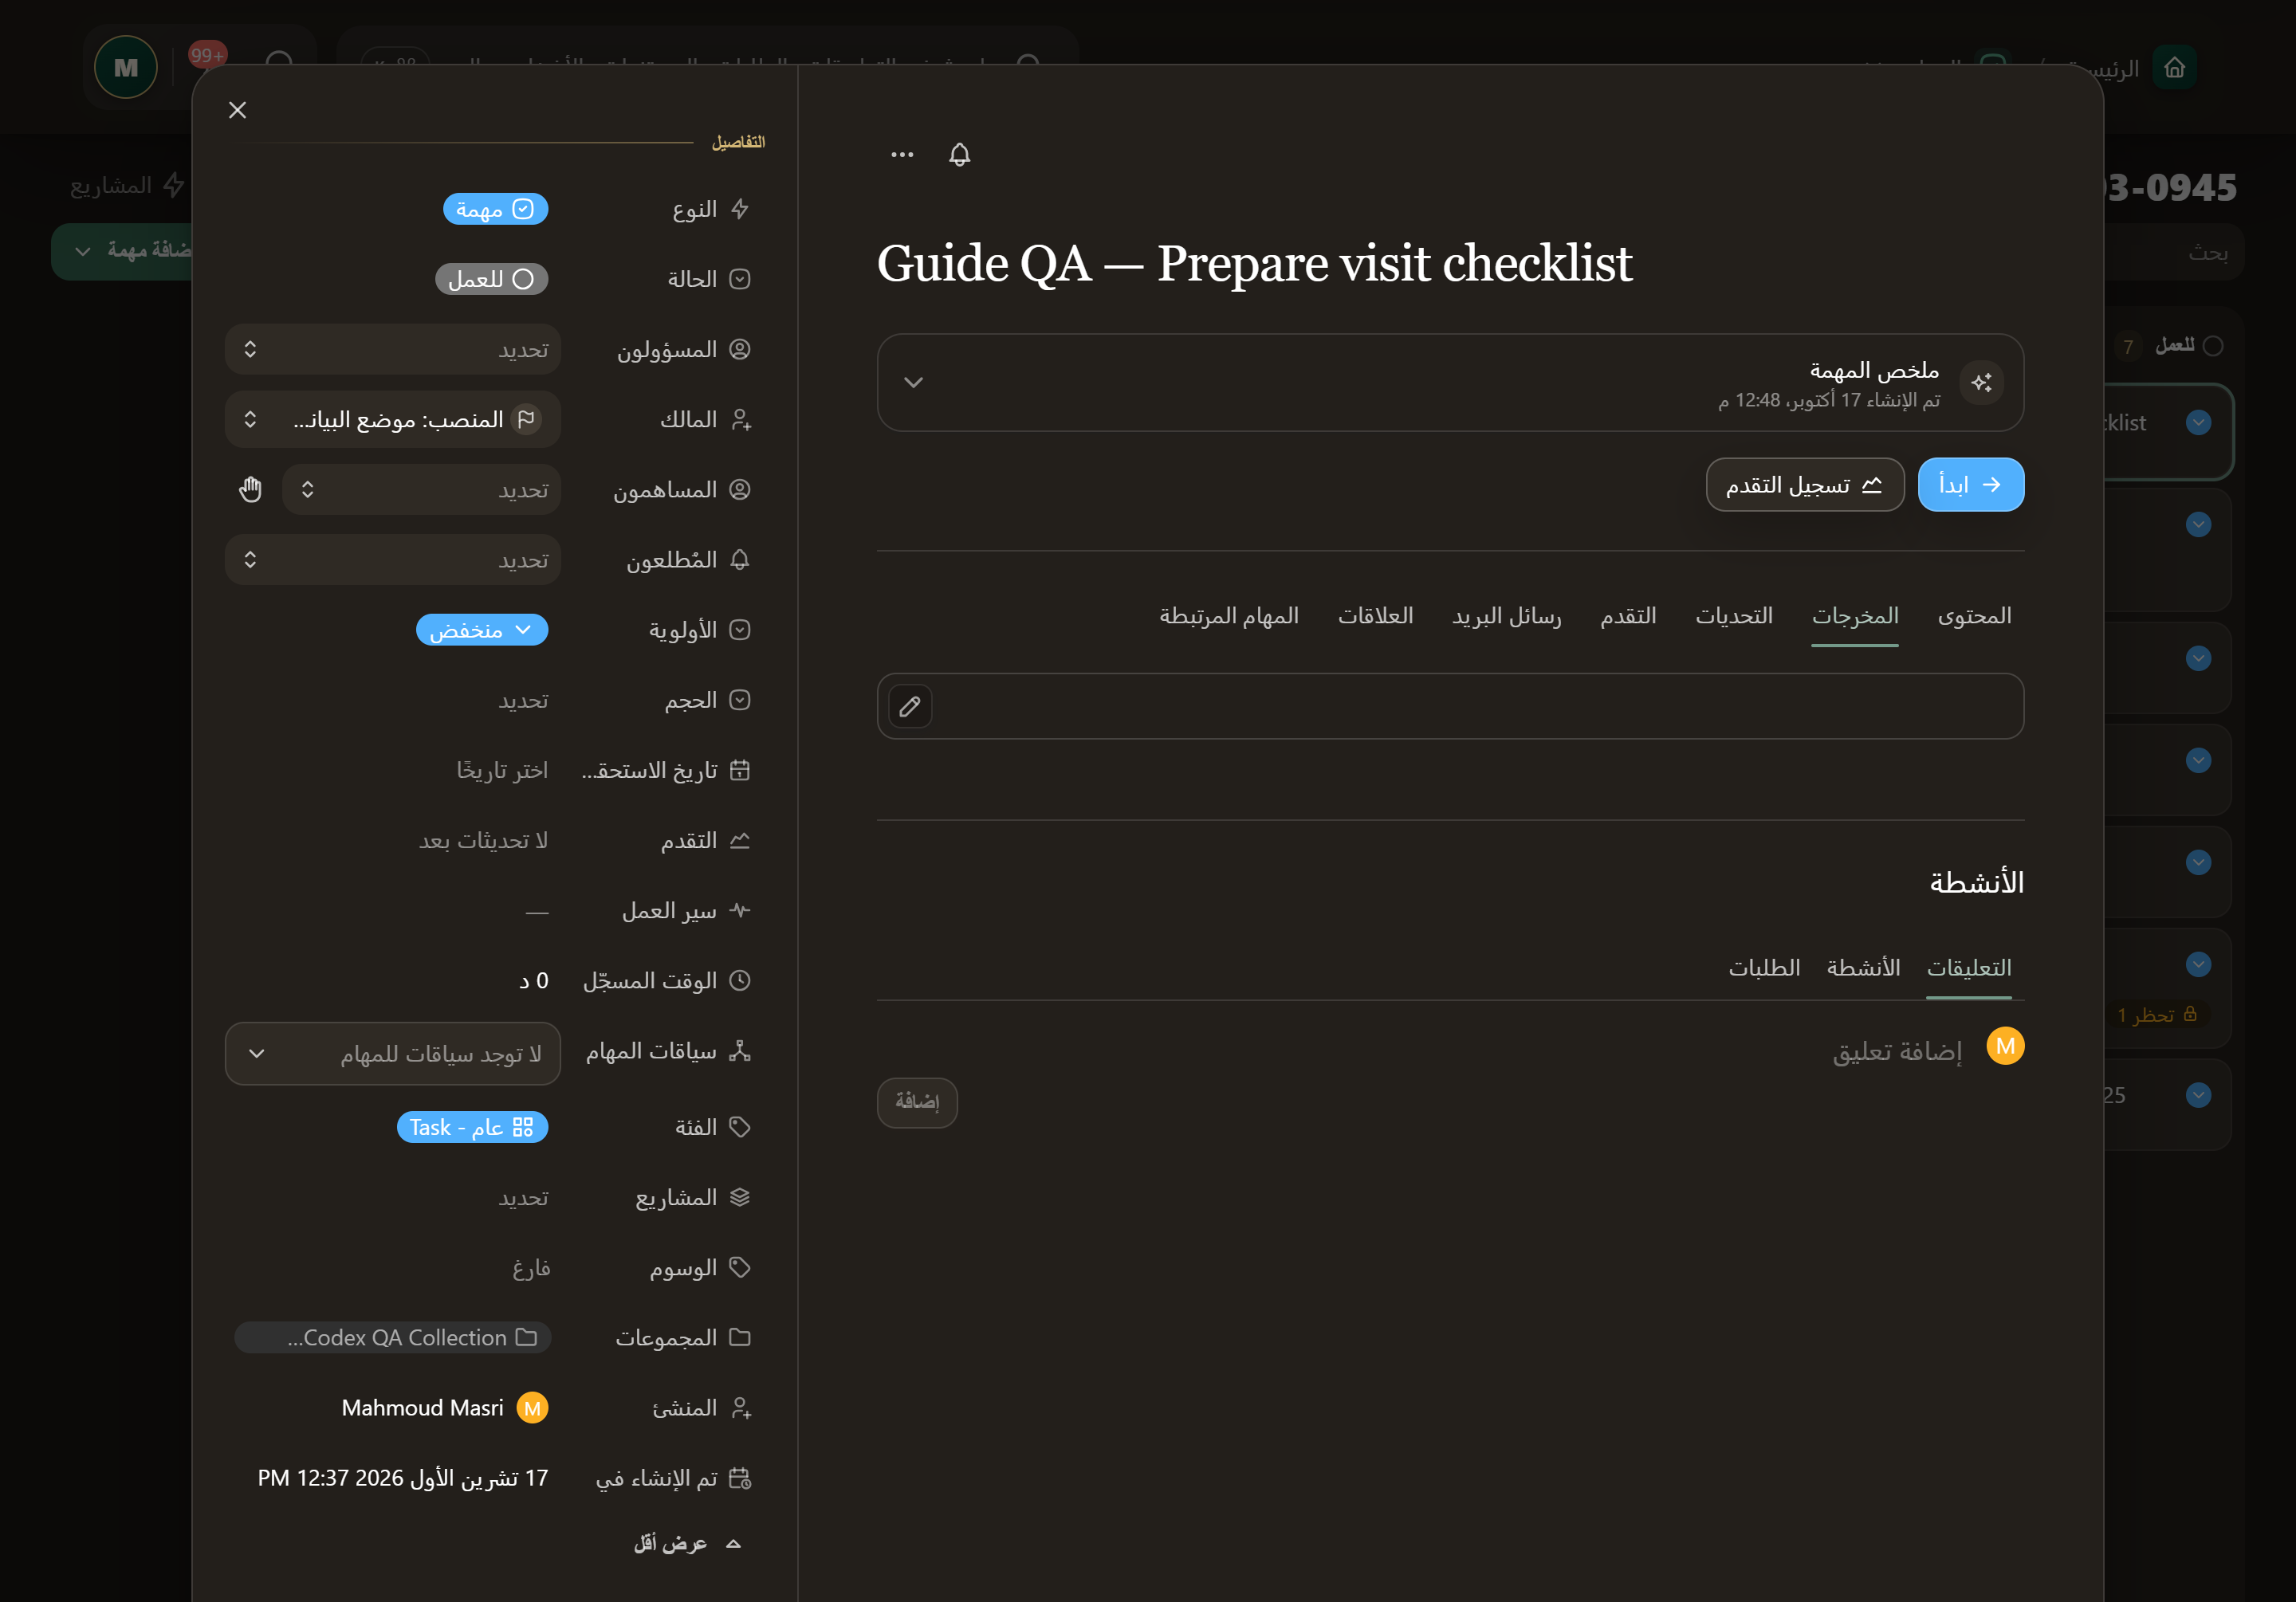
\includegraphics[width=0.95\linewidth,height=0.72\textheight,keepaspectratio]{figures/screens/ch04-output-ar.png}
\caption{المخرجات}
\label{fig:tasks-follow-up-output}
\shotnote{تبويب «المخرجات» هو المكان الذي تسجّل فيه ما نتج عن العمل فعلاً، بعد الضغط على أيقونة التعديل. وبذلك يفصل الفريق بين وصف المطلوب في «المحتوى» والنتيجة المنجزة هنا. ويبقى التبويب فارغاً، كما في هذه المهمة التجريبية، حتى يكتب المنفّذ نتيجته. ① تبويب «المخرجات» داخل المهمة. ② زر الإجراء الرئيسي للمهمة، مثل «ابدأ» أو «إكمال»، ويتغير بحسب حالتها. واكتب في التبويب النتيجة الفعلية للعمل.}
\end{figure}

\begin{figure}[H]
\centering
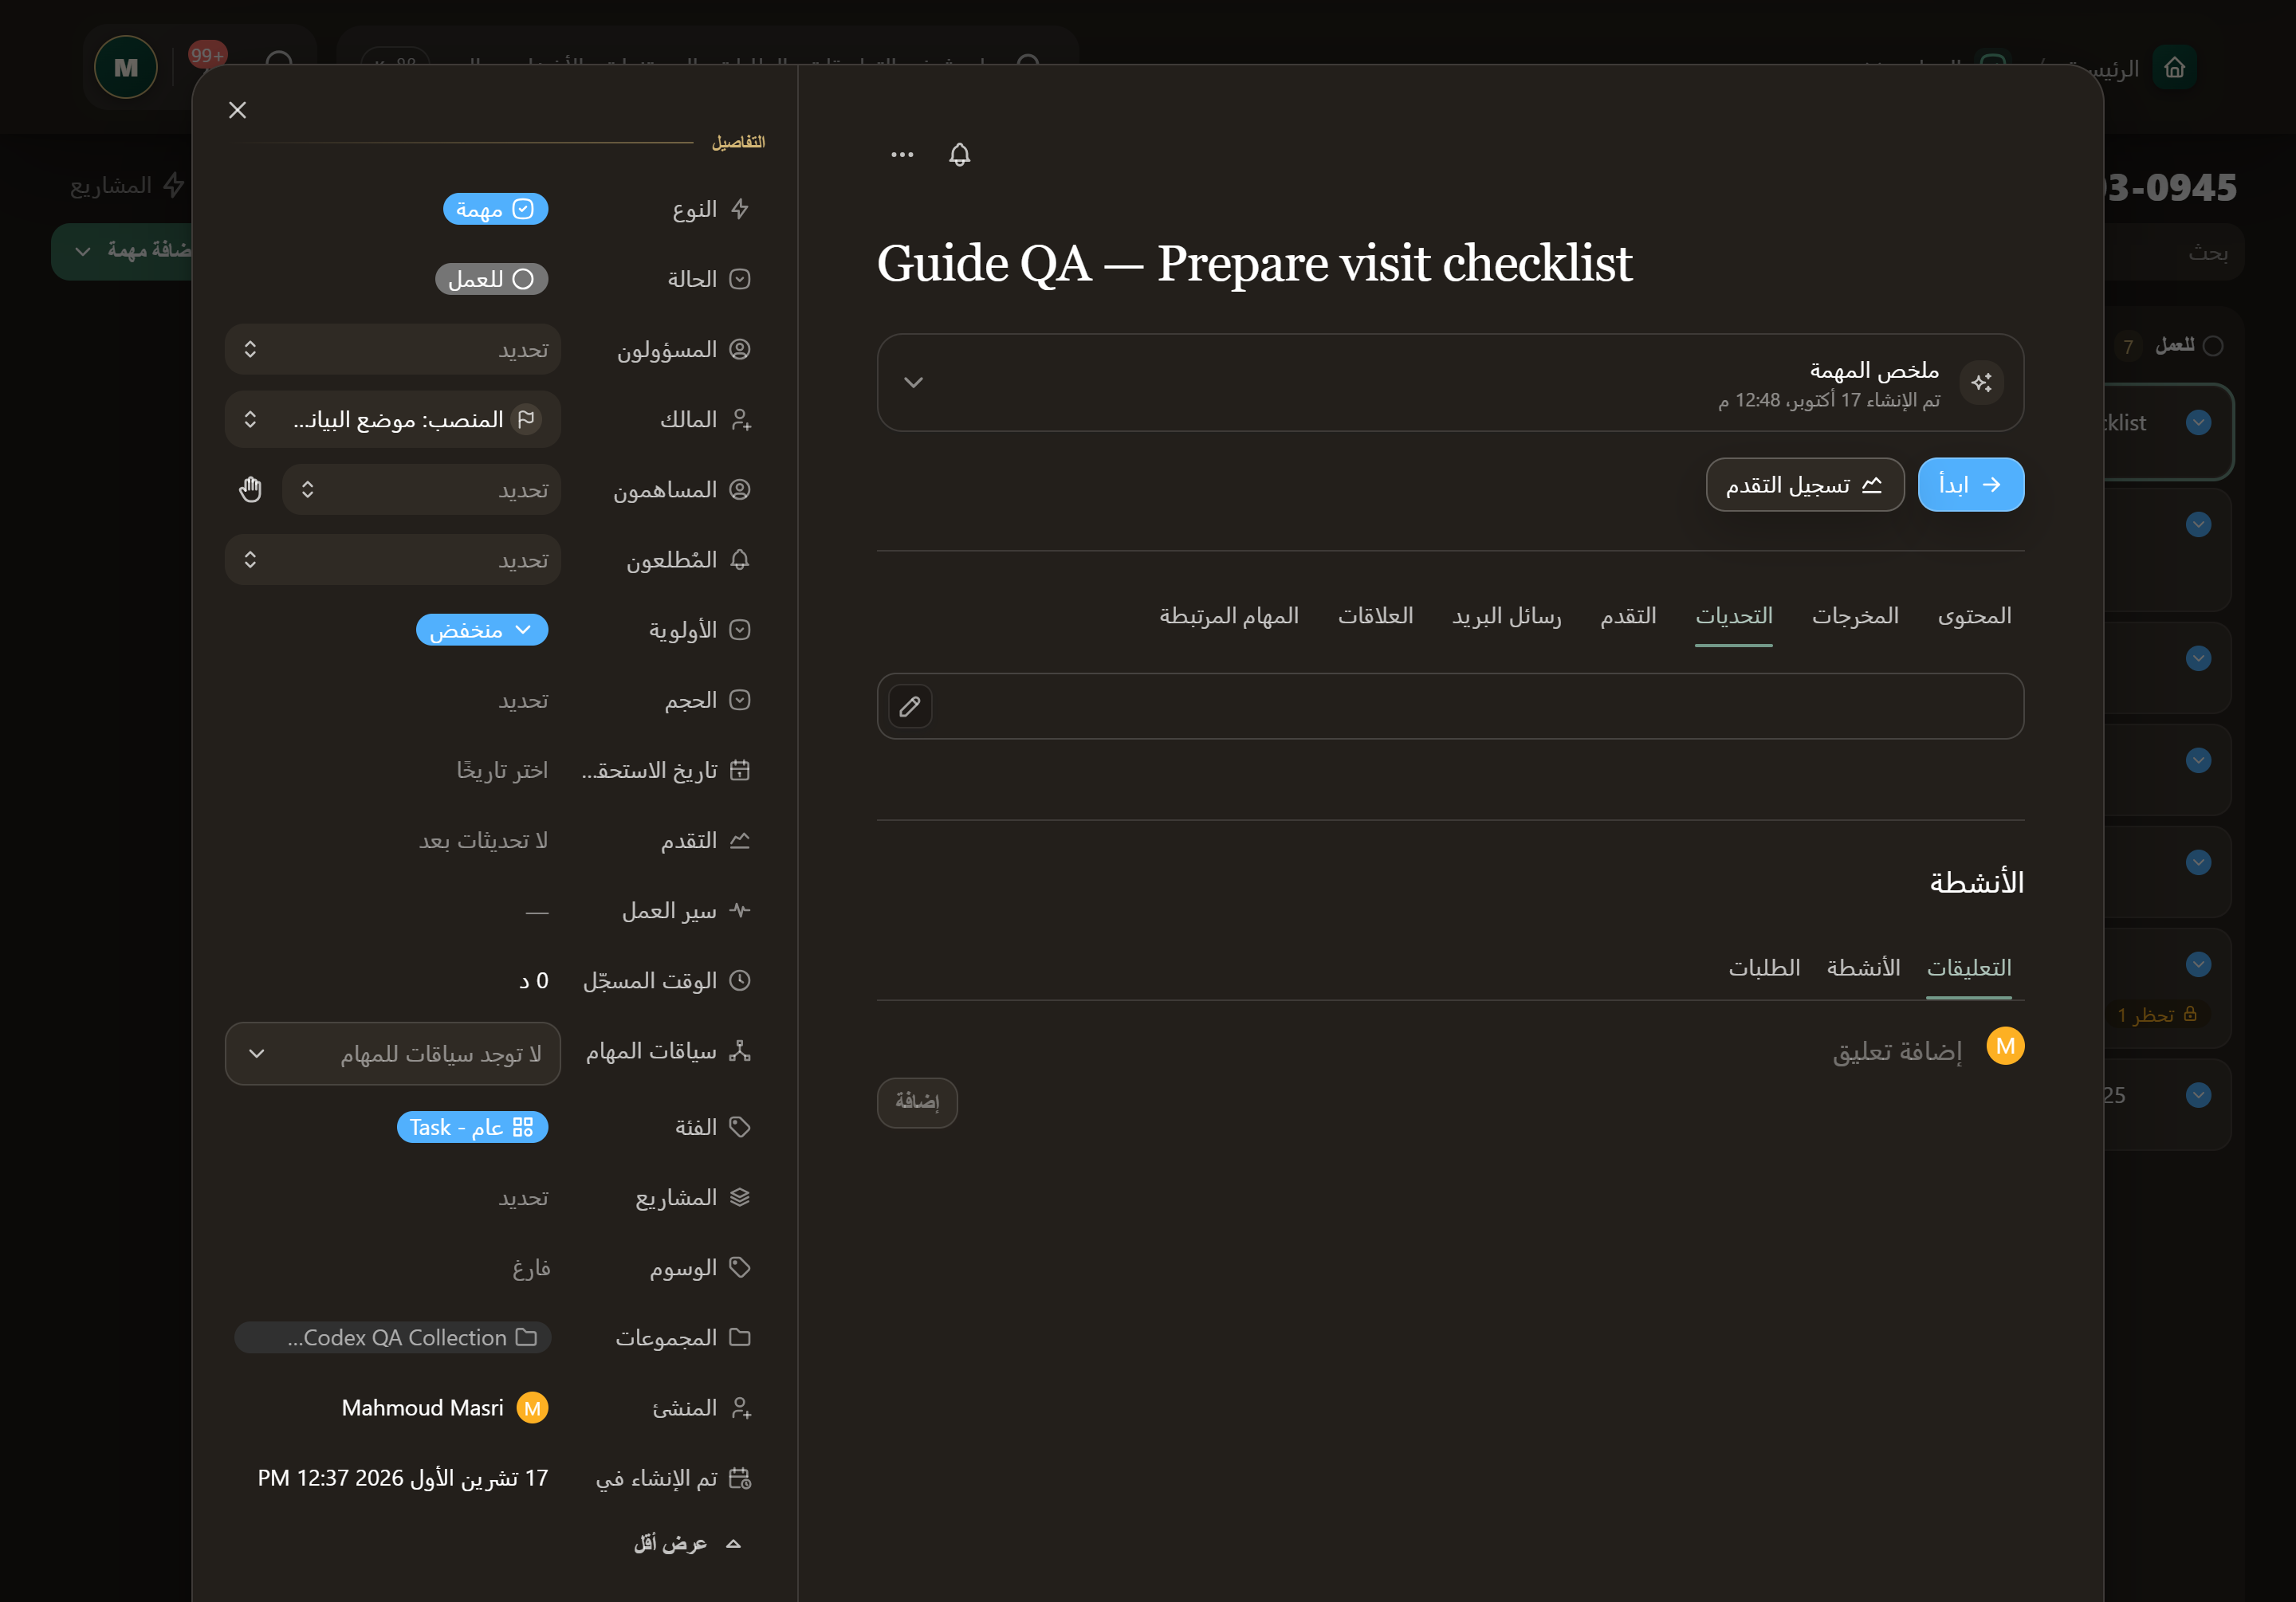
\includegraphics[width=0.95\linewidth,height=0.72\textheight,keepaspectratio]{figures/screens/ch04-challenges-ar.png}
\caption{التحديات}
\label{fig:tasks-follow-up-challenges}
\shotnote{يخصَّص تبويب «التحديات» للعوائق التي تؤخر العمل أو تحتاج قراراً من شخص آخر، وهو فارغ في هذه المهمة التجريبية. ويُطلع تسجيلُ العائق هنا الفريقَ عليه، لكنه لا يغيّر حالة المهمة تلقائياً؛ لذلك غيّر الحالة أو اطلب المساعدة بإجراء مستقل. ① تبويب «التحديات» داخل المهمة. ② زر الإجراء الرئيسي للمهمة، مثل «ابدأ» أو «إكمال»، ويتغير بحسب حالتها. واكتب في التبويب ما يعيق العمل.}
\end{figure}

\begin{figure}[H]
\centering
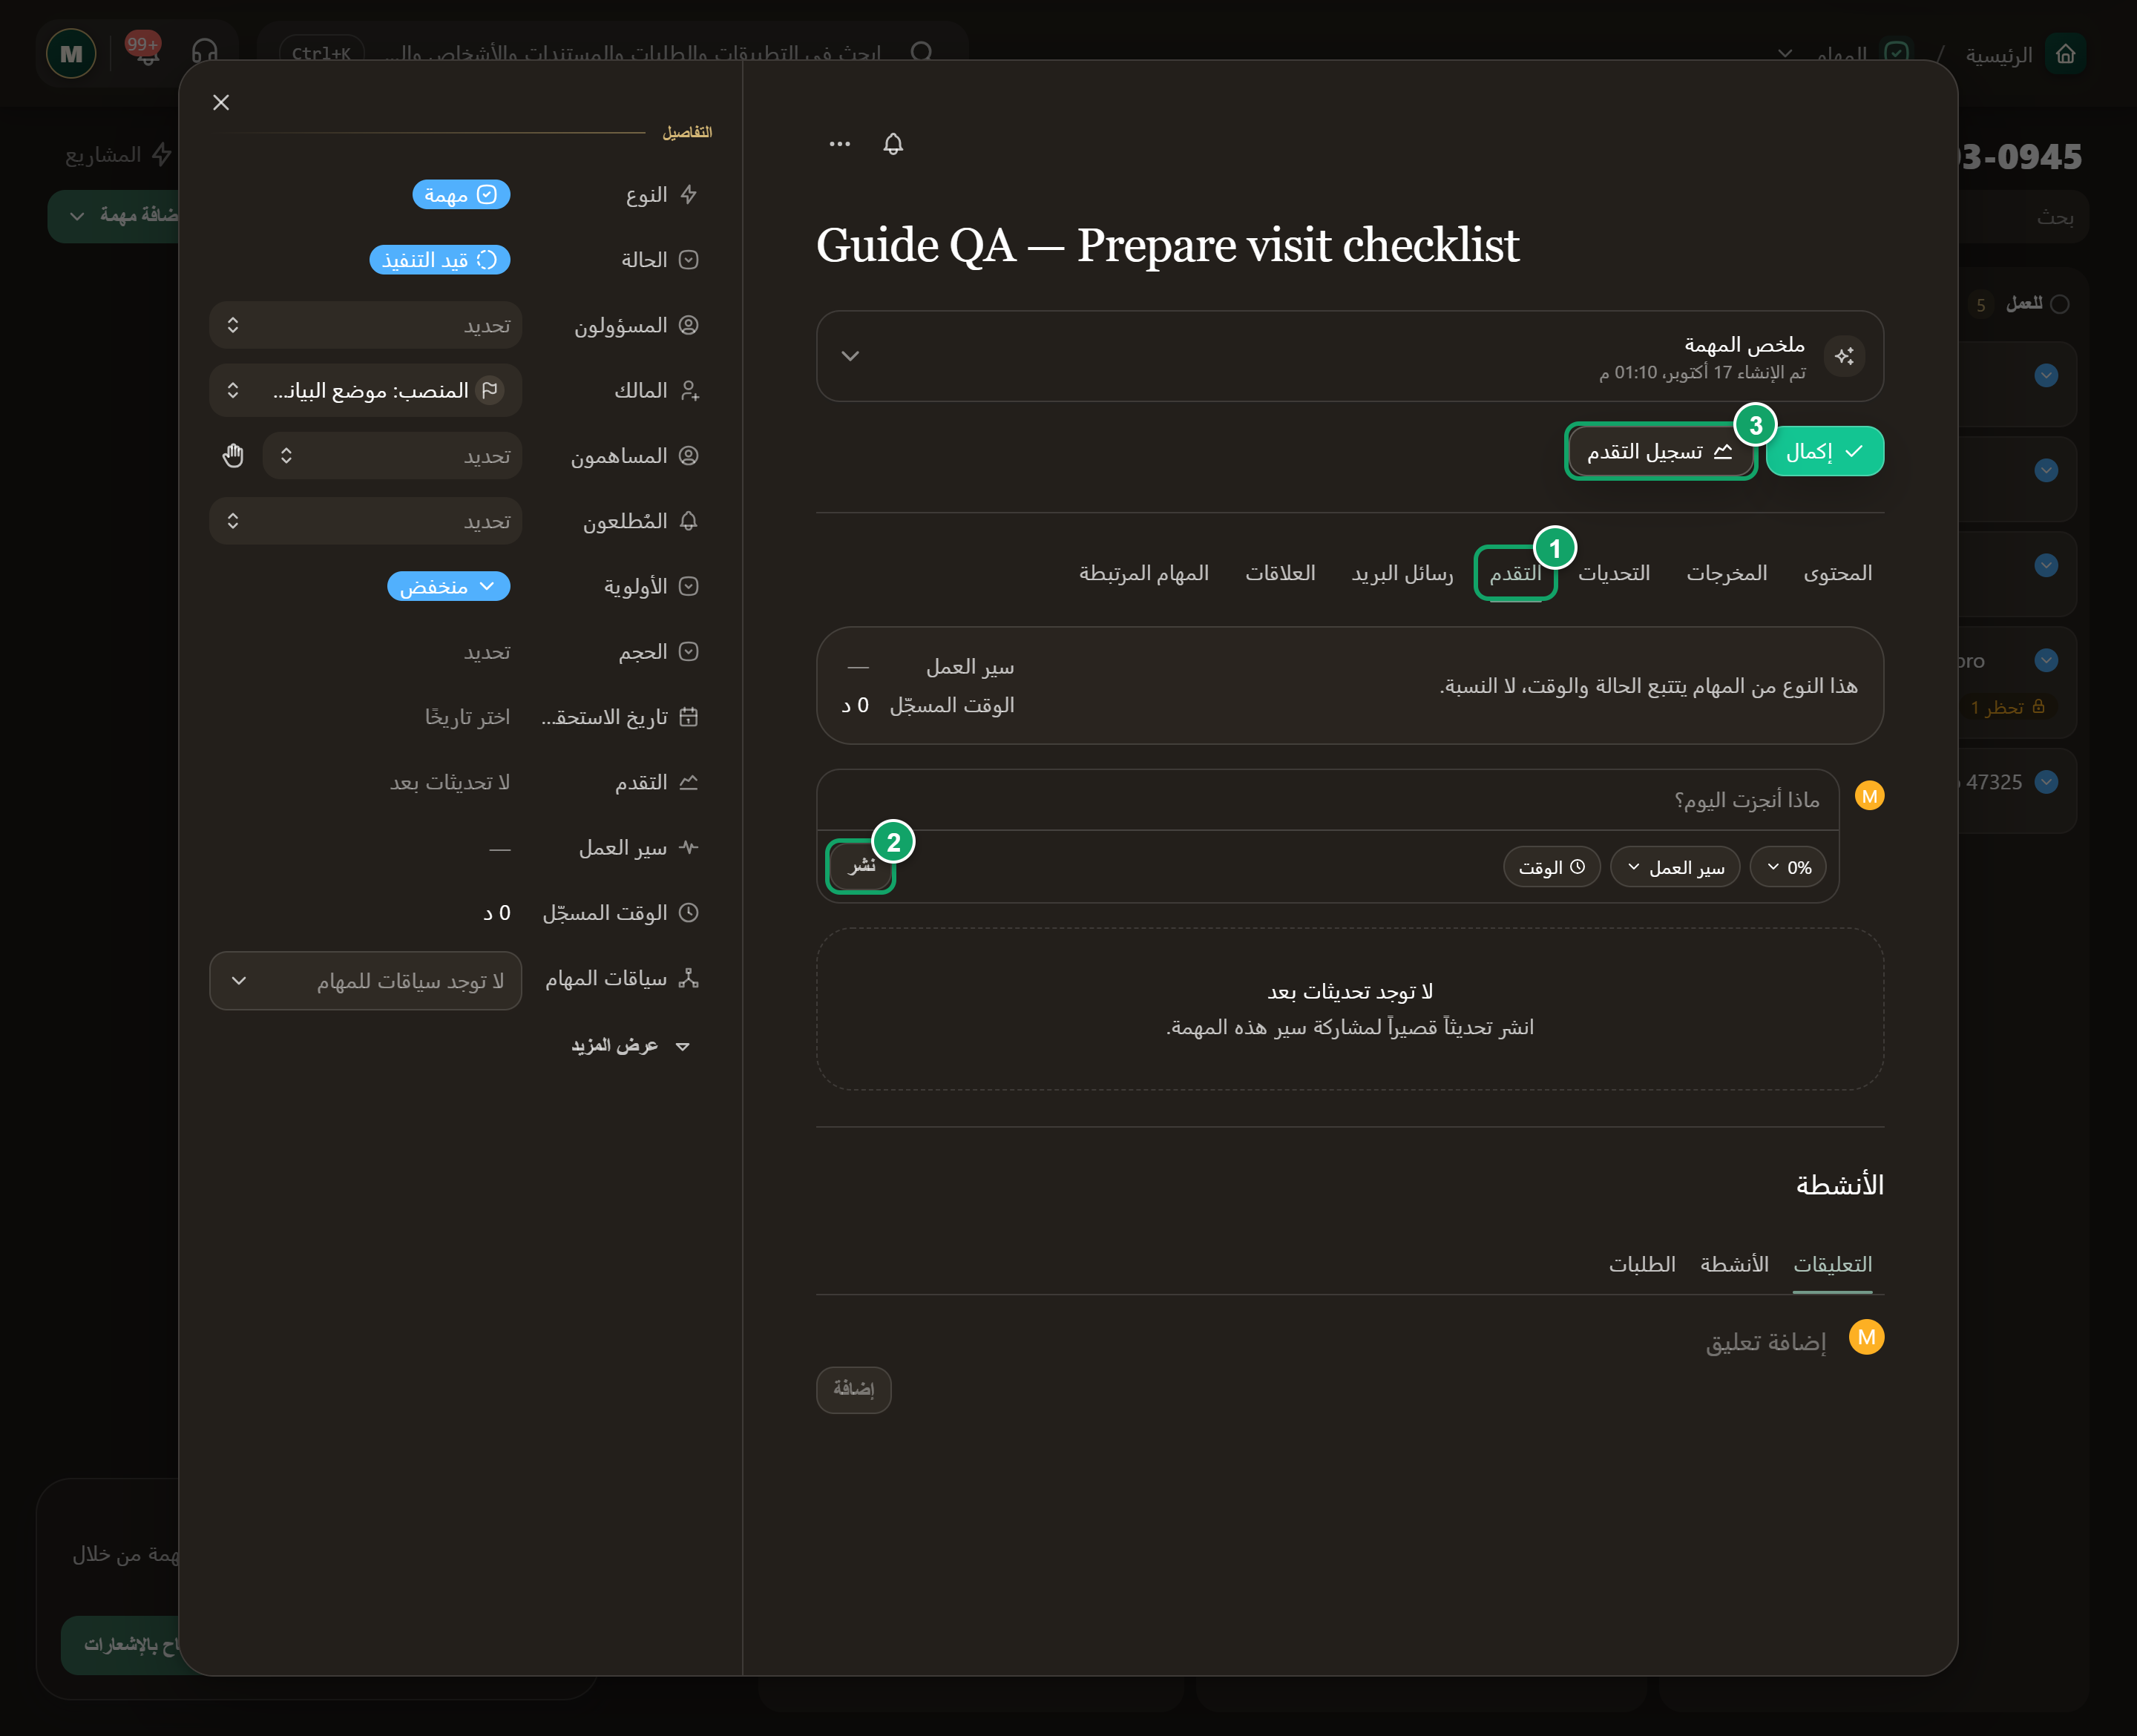
\includegraphics[width=0.95\linewidth,height=0.72\textheight,keepaspectratio]{figures/screens/ch04-progress-ar.png}
\caption{تحديثات التقدم}
\label{fig:tasks-follow-up-progress}
\shotnote{يجمع تبويب «التقدم» التحديثات القصيرة التي ينشرها الفريق عن سير المهمة: تكتب في «ماذا أنجزت اليوم؟» ثم تضغط «نشر». ويحدد نوع المهمة ما يُتتبَّع، فنوع هذه المهمة مثلاً يتتبع الحالة والوقت لا النسبة. ولا توجد تحديثات بعد في هذه المهمة التجريبية. ① تبويب «التقدم». ② «نشر»: يرسل التحديث بعد كتابة ما أنجزته والنسبة وسير العمل. ③ «تسجيل التقدم»: يفتح التحديث من أعلى المهمة.}
\end{figure}

\begin{figure}[H]
\centering
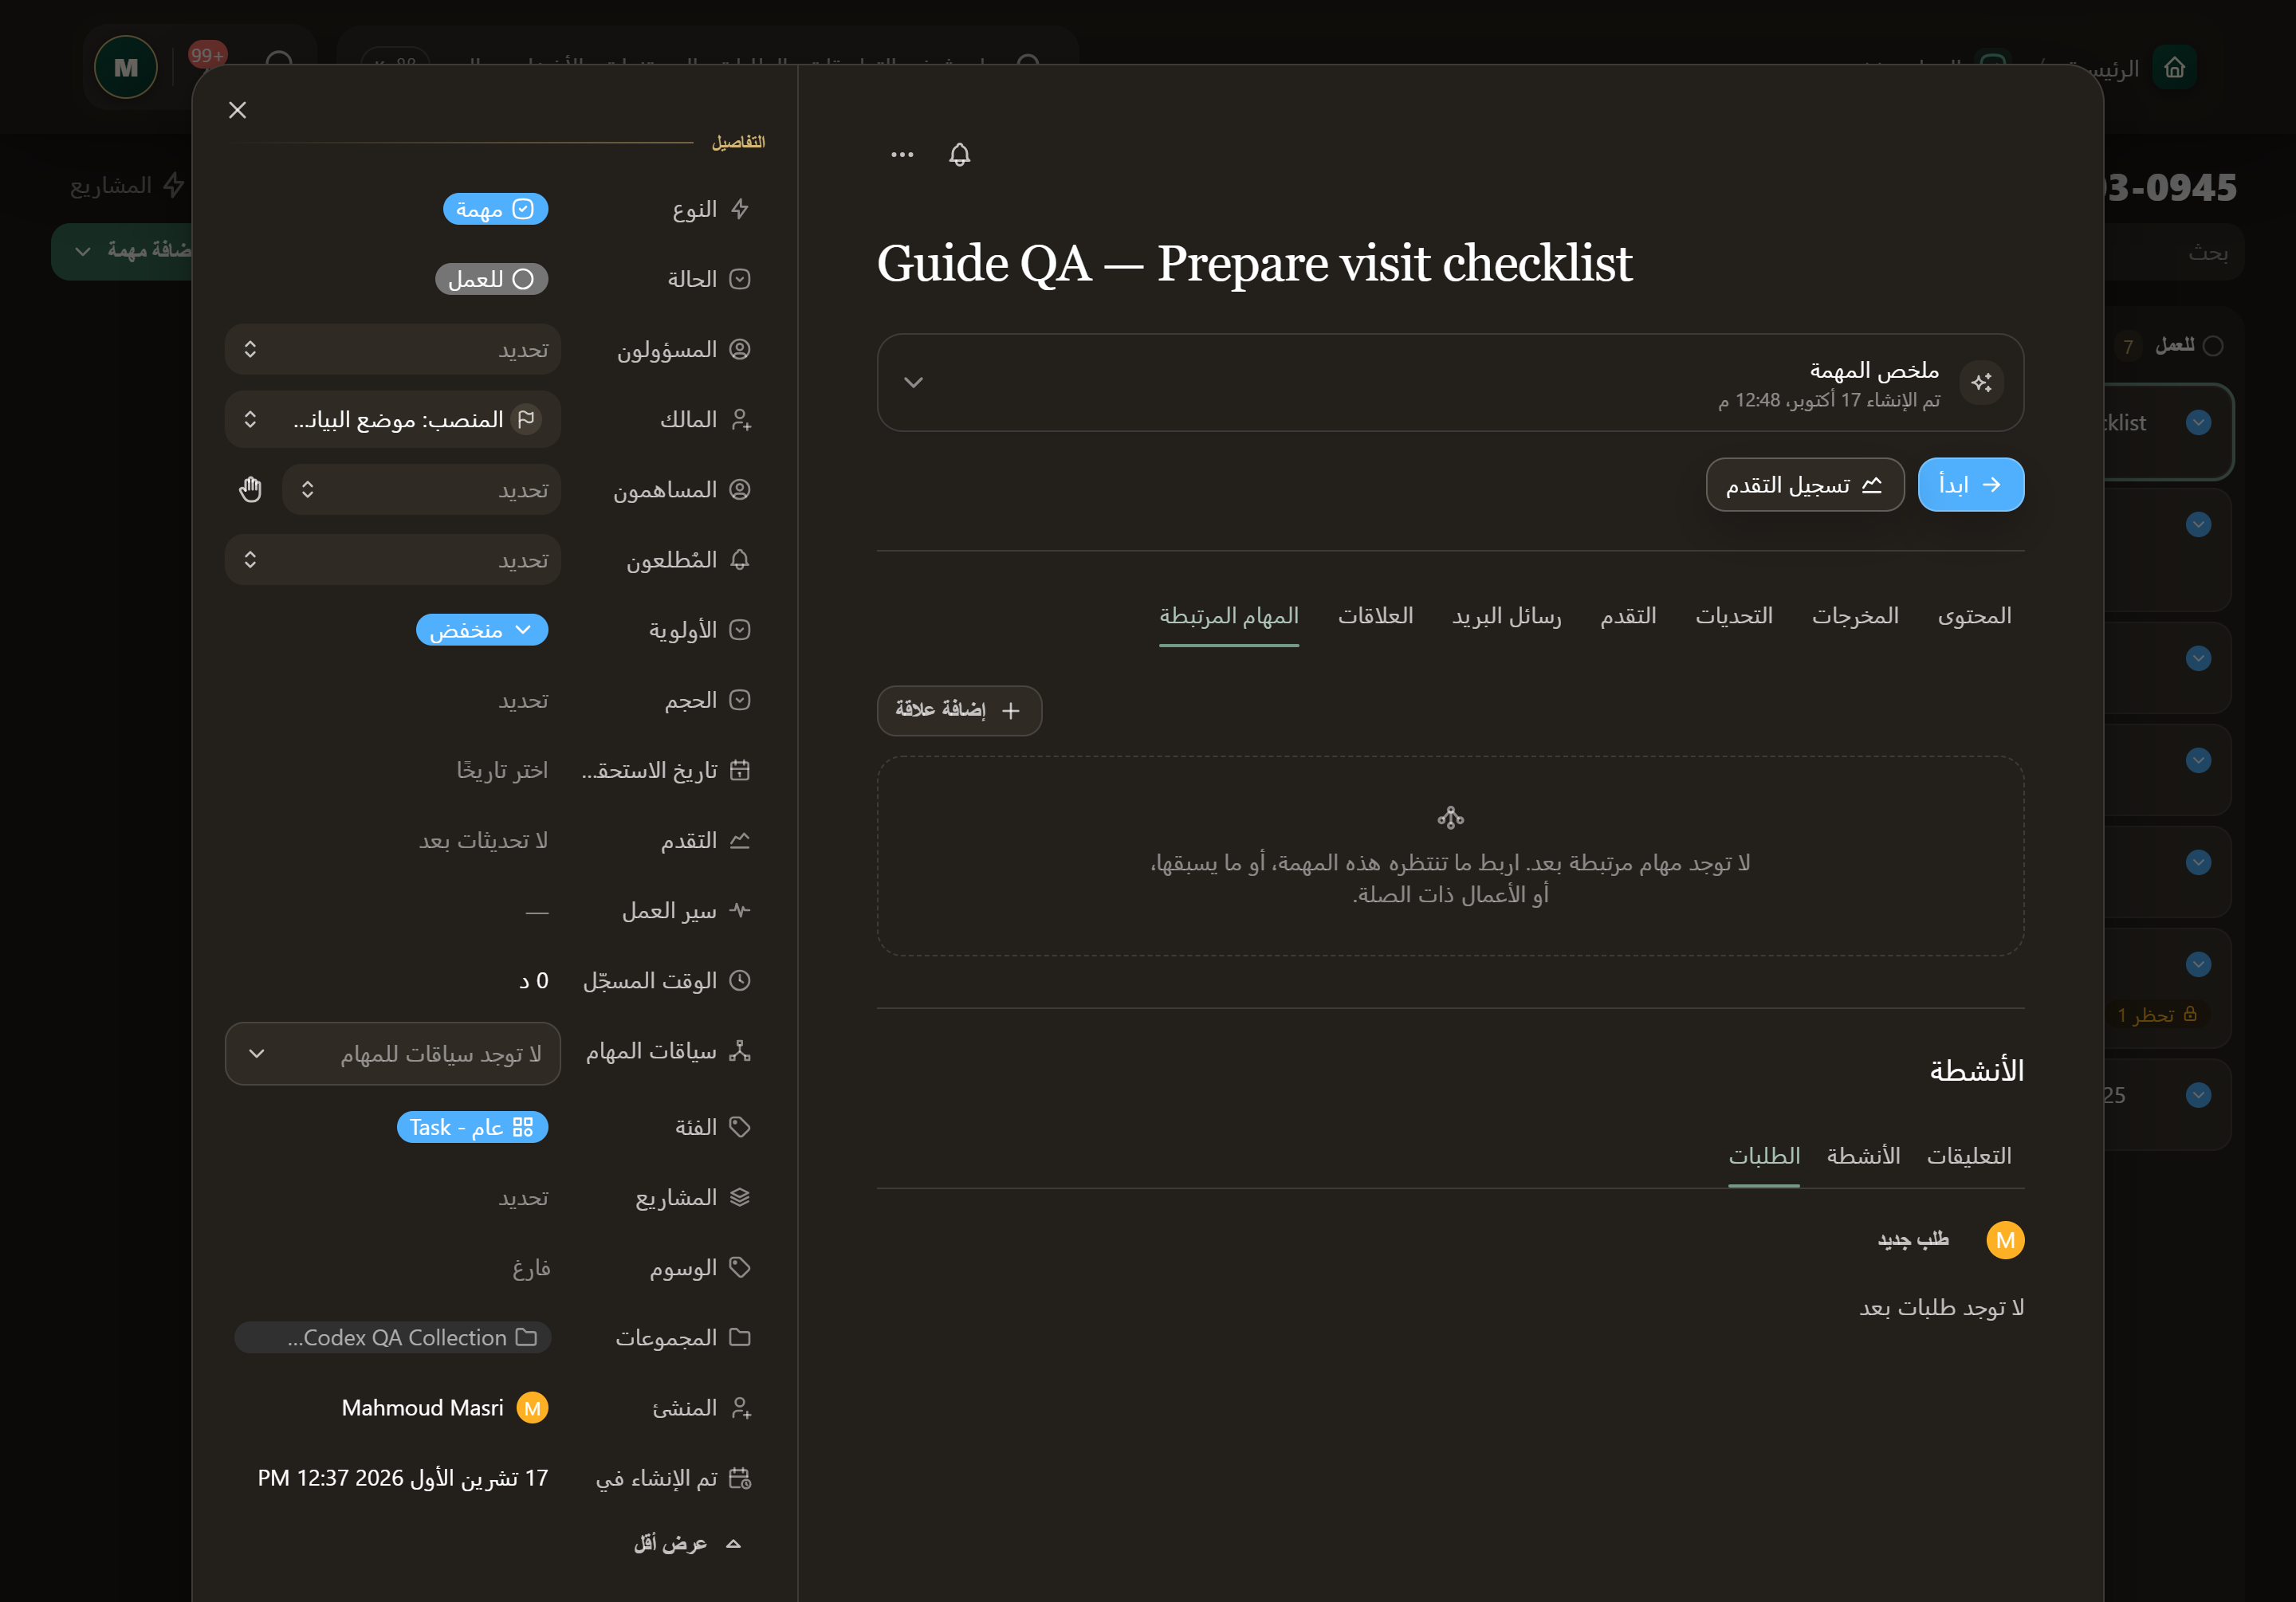
\includegraphics[width=0.95\linewidth,height=0.72\textheight,keepaspectratio]{figures/screens/ch04-requests-ar.png}
\caption{الطلبات داخل المهمة}
\label{fig:tasks-follow-up-requests}
\shotnote{تتيح «الطلبات» أن تطلب من عضو آخر إجراءً محدداً داخل سجل المهمة نفسه عبر «طلب جديد»، فيبقى الطلب ورده مرتبطين بالعمل بدلاً من ضياعهما في المراسلات. وحالة الطلب مستقلة عن حالة المهمة، ولا توجد طلبات في هذه المهمة التجريبية. ① تبويب «الطلبات». ② «طلب جديد»: يطلب من زميل عملاً أو معلومة مرتبطة بالمهمة.}
\end{figure}

\begin{figure}[H]
\centering
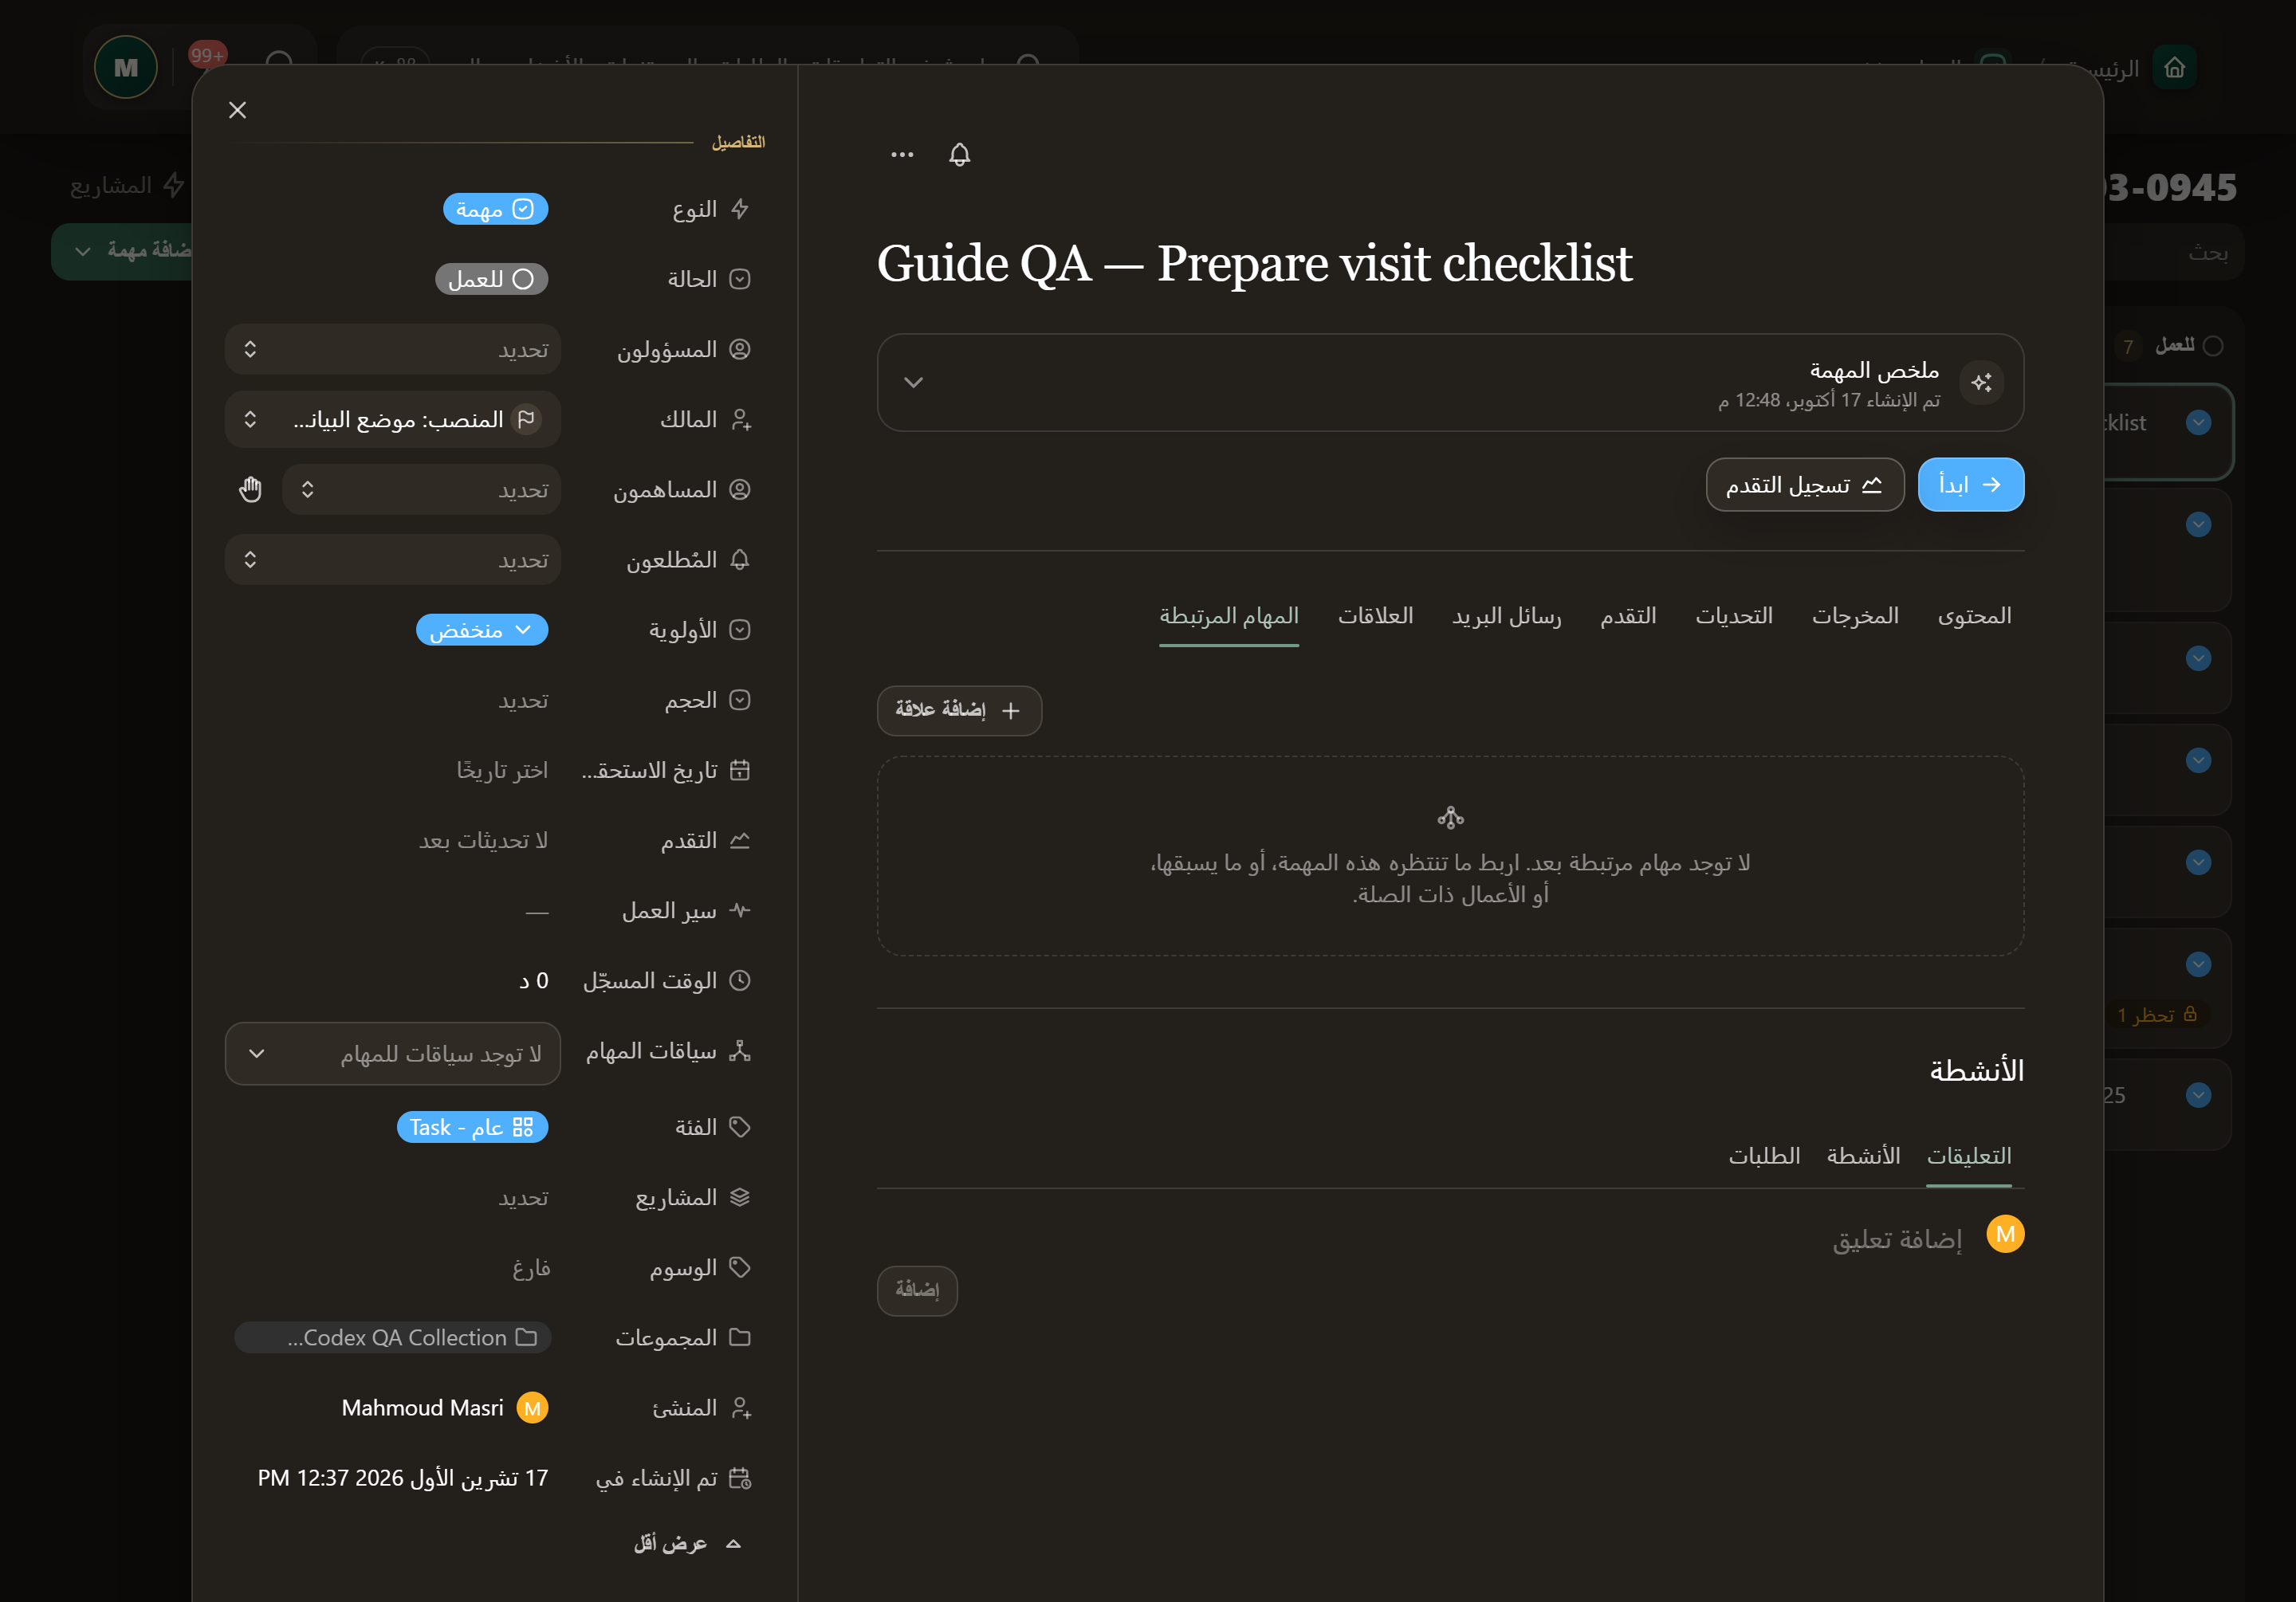
\includegraphics[width=0.95\linewidth,height=0.72\textheight,keepaspectratio]{figures/screens/ch04-comments-ar.png}
\caption{التعليقات}
\label{fig:tasks-follow-up-comments}
\shotnote{تجمع «التعليقات» نقاش الفريق حول المهمة: اكتب في «إضافة تعليق» ثم اضغط «إضافة». ويفيد التعليق في شرح القرارات وطرح الأسئلة، لكنه لا يغيّر حالة المهمة ولا يغني عن تسجيل النتيجة في «المخرجات». ① تبويب «التعليقات». ② «إضافة».}
\end{figure}

\begin{figure}[H]
\centering
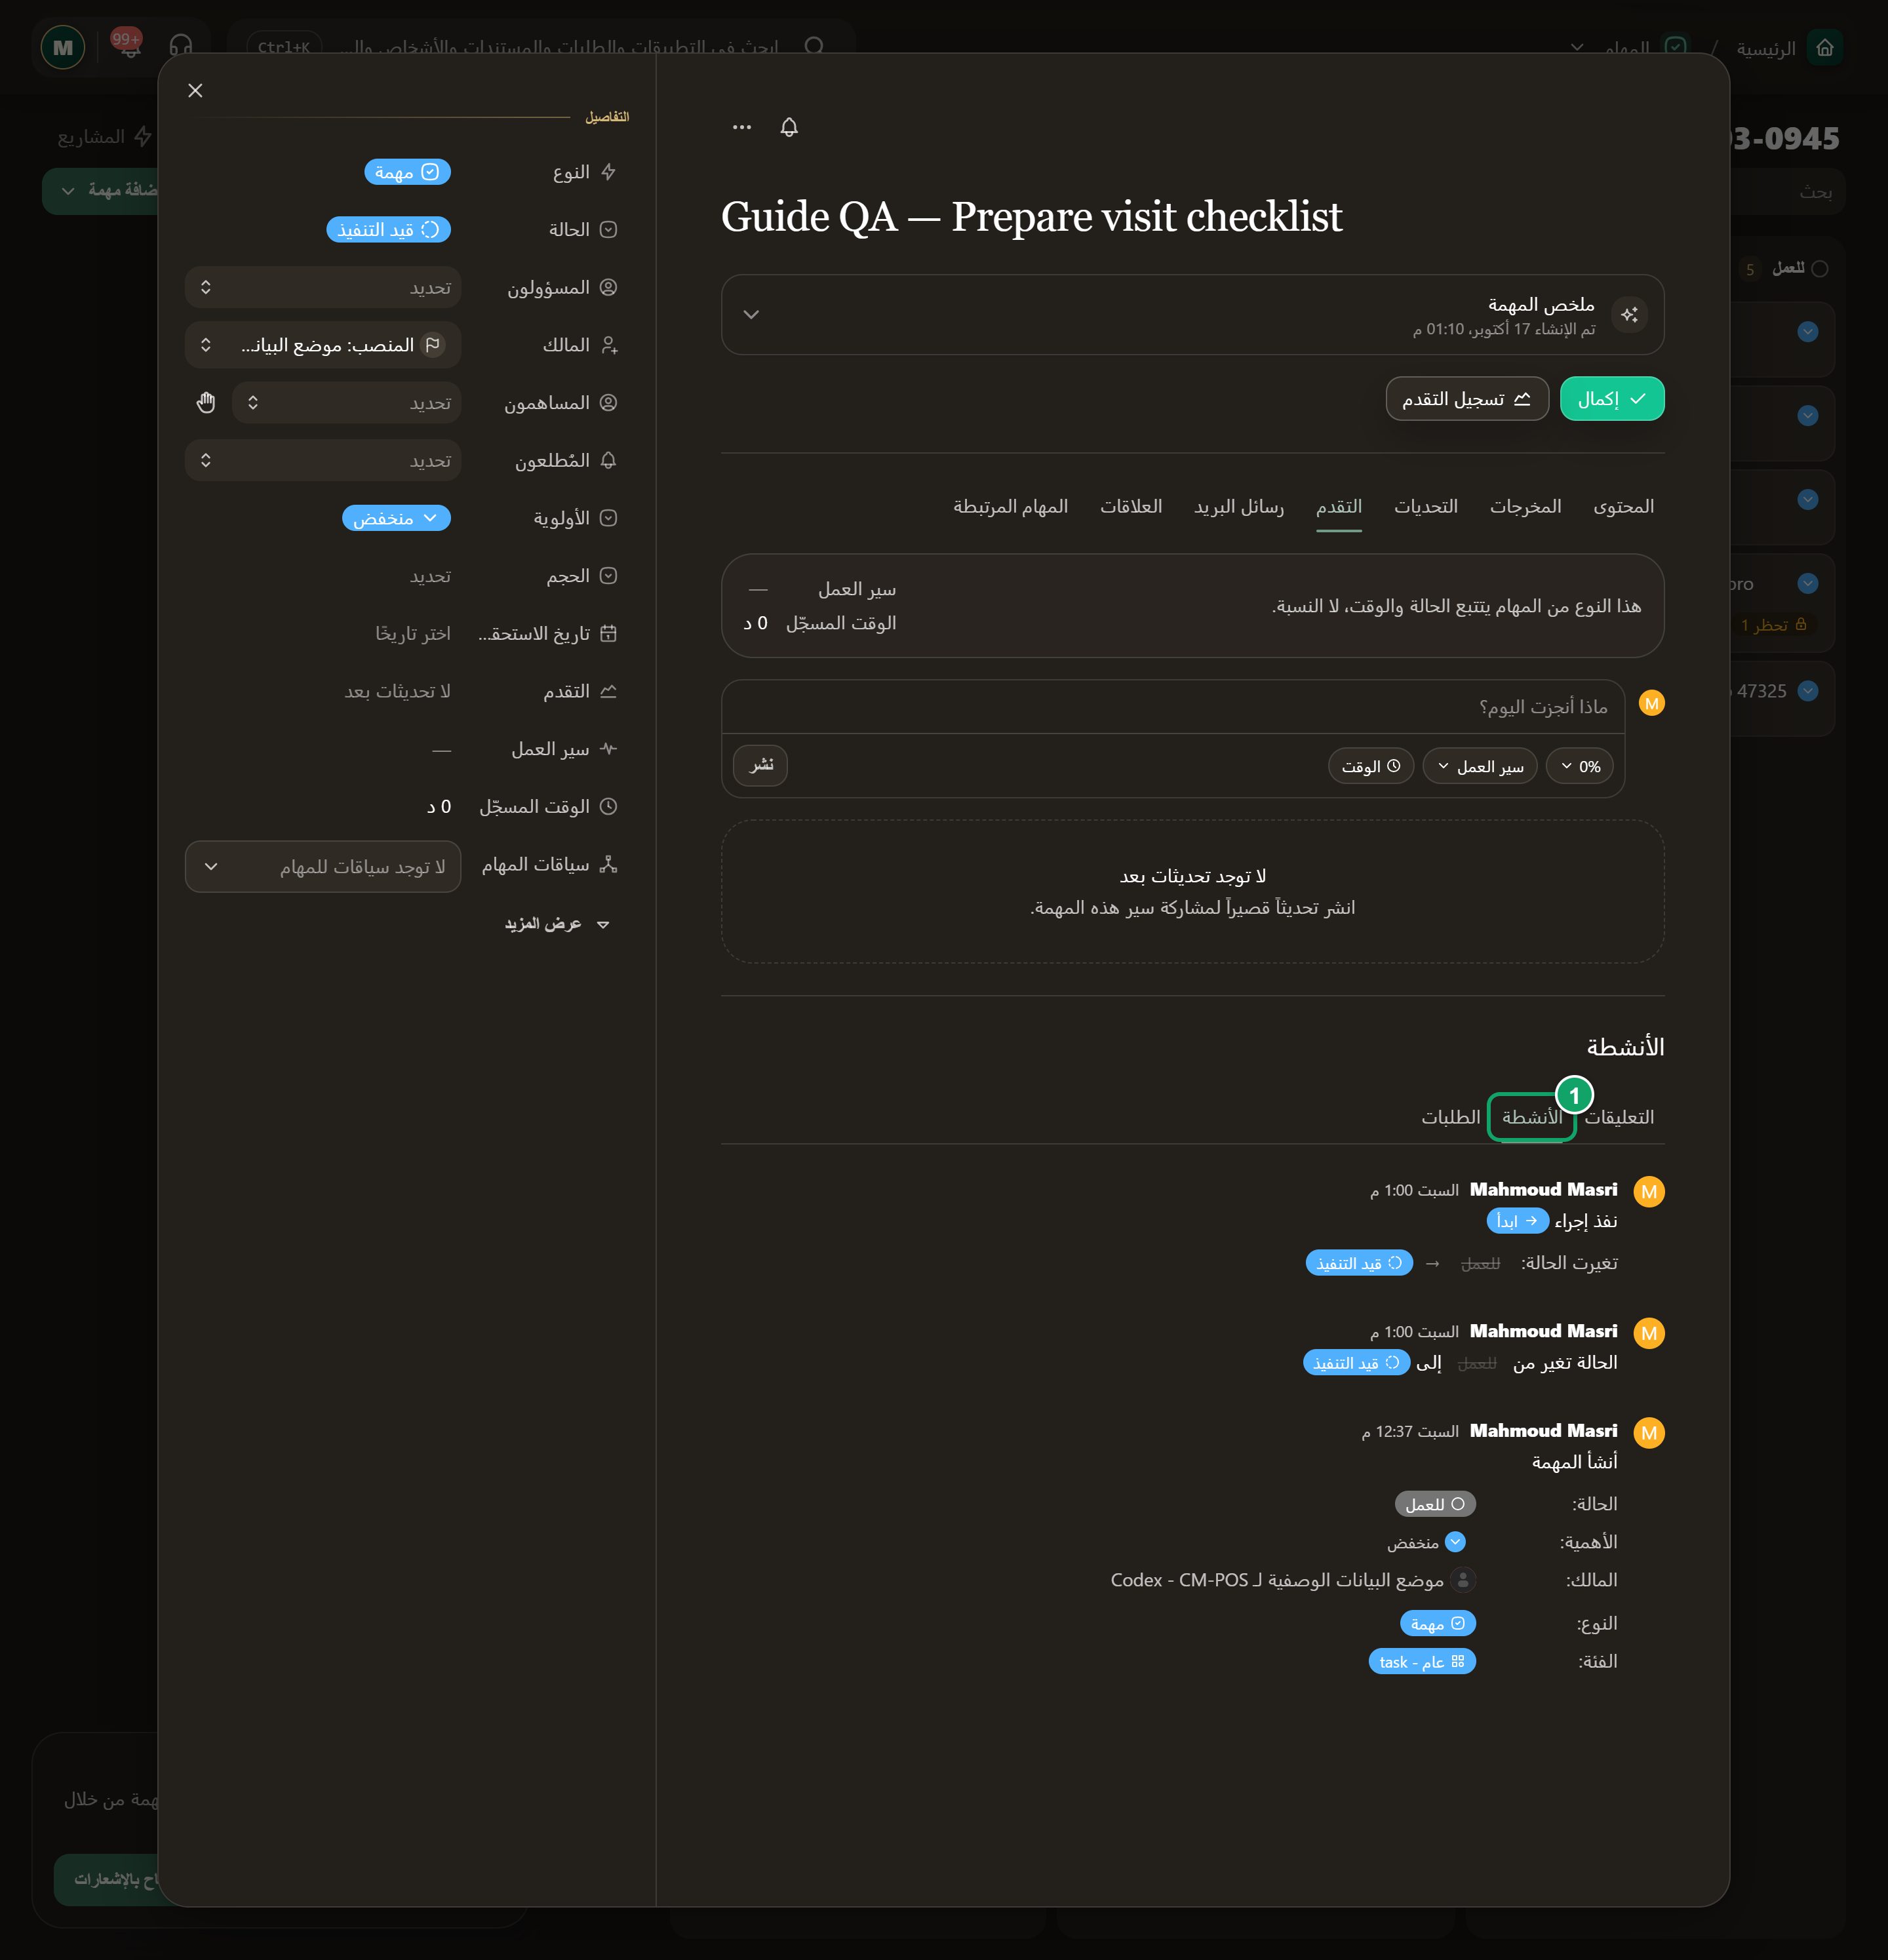
\includegraphics[width=0.95\linewidth,height=0.72\textheight,keepaspectratio]{figures/screens/ch04-activity-ar.png}
\caption{سجل الأنشطة}
\label{fig:tasks-follow-up-activity}
\shotnote{يعرض تبويب «الأنشطة» سجلاً زمنياً لما جرى على المهمة ومن قام به؛ فهنا يظهر حدث «أنشأ المهمة» مع قيمها الأولى مثل الحالة والمالك والنوع. ويرجع إليه المسؤول عندما يسأل عن تغيير ما، أما نتيجة العمل فتُكتب في «المخرجات» لا هنا. الرقم في الصورة: ① تبويب «الأنشطة» الذي يسجّل كل تغيير على المهمة ومن أجراه ومتى.}
\end{figure}

\begin{table}[H]
\centering
\caption{ما الذي تجده هنا؟}
\label{tab:tasks-follow-up-data}
\begin{tabularx}{\linewidth}{R{3.6cm} Y}
\rcHeaderRow
\thh{القسم} & \thh{المحتوى والإجراء}\\
الوصف والمخرجات والتحديات & سياق التنفيذ، ثم نتيجته، ثم عوائقه. ويدعم محرر المحتوى الملفات حيث تتوفر أدوات الإرفاق.\\
التقدم & تحديثات مؤرخة، ونسبة الإنجاز، و«سير العمل»، والوقت، والخطوات التالية، والعوائق؛ بحسب إعداد النوع.\\
التعليقات والأنشطة & نقاش العمل وسجل التغييرات. ويتيح لك زر المتابعة أن تتابع المهمة أو تلغي متابعتها.\\
الطلبات والملخص & طلب مساهمة أو رد من عضو آخر، وحالة الطلب مستقلة عن حالة المهمة. أما «ملخص المهمة» المساعد فيحتاج إلى مراجعة ولا يحل محل السجل.\\
\end{tabularx}
\end{table}

\begin{figure}[H]
\centering
\begin{tikzpicture}[node distance=0.5cm]
\node[stepBox] (a) {\RL{تسجيل النتيجة}};
\node[stepBox,below=of a] (b) {\RL{معالجة العائق}};
\node[stepBox,below=of b] (c) {\RL{مراجعة الحالة}};
\draw[flowsTo] (a) -- (b);
\draw[flowsTo] (b) -- (c);
\end{tikzpicture}
\rclegend
\caption{خطوات الاستخدام}
\label{fig:tasks-follow-up-flow}
\shotnote{يبيّن المخطط ترتيب المتابعة: سجّل النتيجة أولاً ليتضح ما أُنجز، ثم عالج العائق إن وُجد، وبعدها راجع الحالة واختر الانتقال المناسب. فتغيير الحالة قبل معالجة العائق يعطي الفريق صورة غير دقيقة عن وضع العمل.}
\end{figure}

\subsection{خطوات العمل والتحقق}
\begin{enumerate}
\item افتح «المخرجات» واضغط أيقونة التعديل، ثم سجّل النتيجة واحفظ. واستخدم «التحديات» بالطريقة نفسها عند وجود عائق.
\item إذا ظهر زر «تسجيل التقدم»، فافتحه وأدخل التحديث والحقول المطلوبة ثم احفظ، وتحقق من ظهوره في «التقدم».
\item للنقاش اكتب تعليقاً ثم اضغط «إضافة». ولطلب إجراء افتح «الطلبات»، وحدد العضو ونص الطلب، ثم أرسله وتابع حالته.
\item بعد مراجعة النتيجة استخدم انتقال الحالة المتاح، وإذا رُفض الانتقال فراجع العوائق والعلاقات المطلوبة.
\end{enumerate}

\textbf{تحقق ومعالجة المشكلة:} أعد فتح المهمة للتحقق من النتيجة والتحديث والحالة. واعلم أن اكتمال المهمة لا يعني موافقة رسمية أو توقيعاً على سجل آخر.

\clearpage
\section{العلاقات والسجلات المرتبطة}
\label{sec:tasks-feature-relationships}

تربط العلاقات المهمة بمصدر العمل أو بدليل إنجازه أو بمهمة أخرى. حدد معنى العلاقة قبل اختيار السجل، حتى يفهم الفريق سبب الربط.

\textbf{المسار ومن يستخدمه:} مهمة ← «العلاقات» أو «المهام المرتبطة» أو «رسائل البريد». يستخدمها المحرر المخوّل.

\begin{rcnote}[مثال: شركة الأفق]
تربط سارة مهمة تجهيز القائمة بسجل الزيارة، وتوضح أن تأكيد العنوان يجب أن يسبق التنفيذ، فيعرف عمر ما ينتظره وأين يجد المصدر.
\end{rcnote}

\begin{figure}[H]
\centering
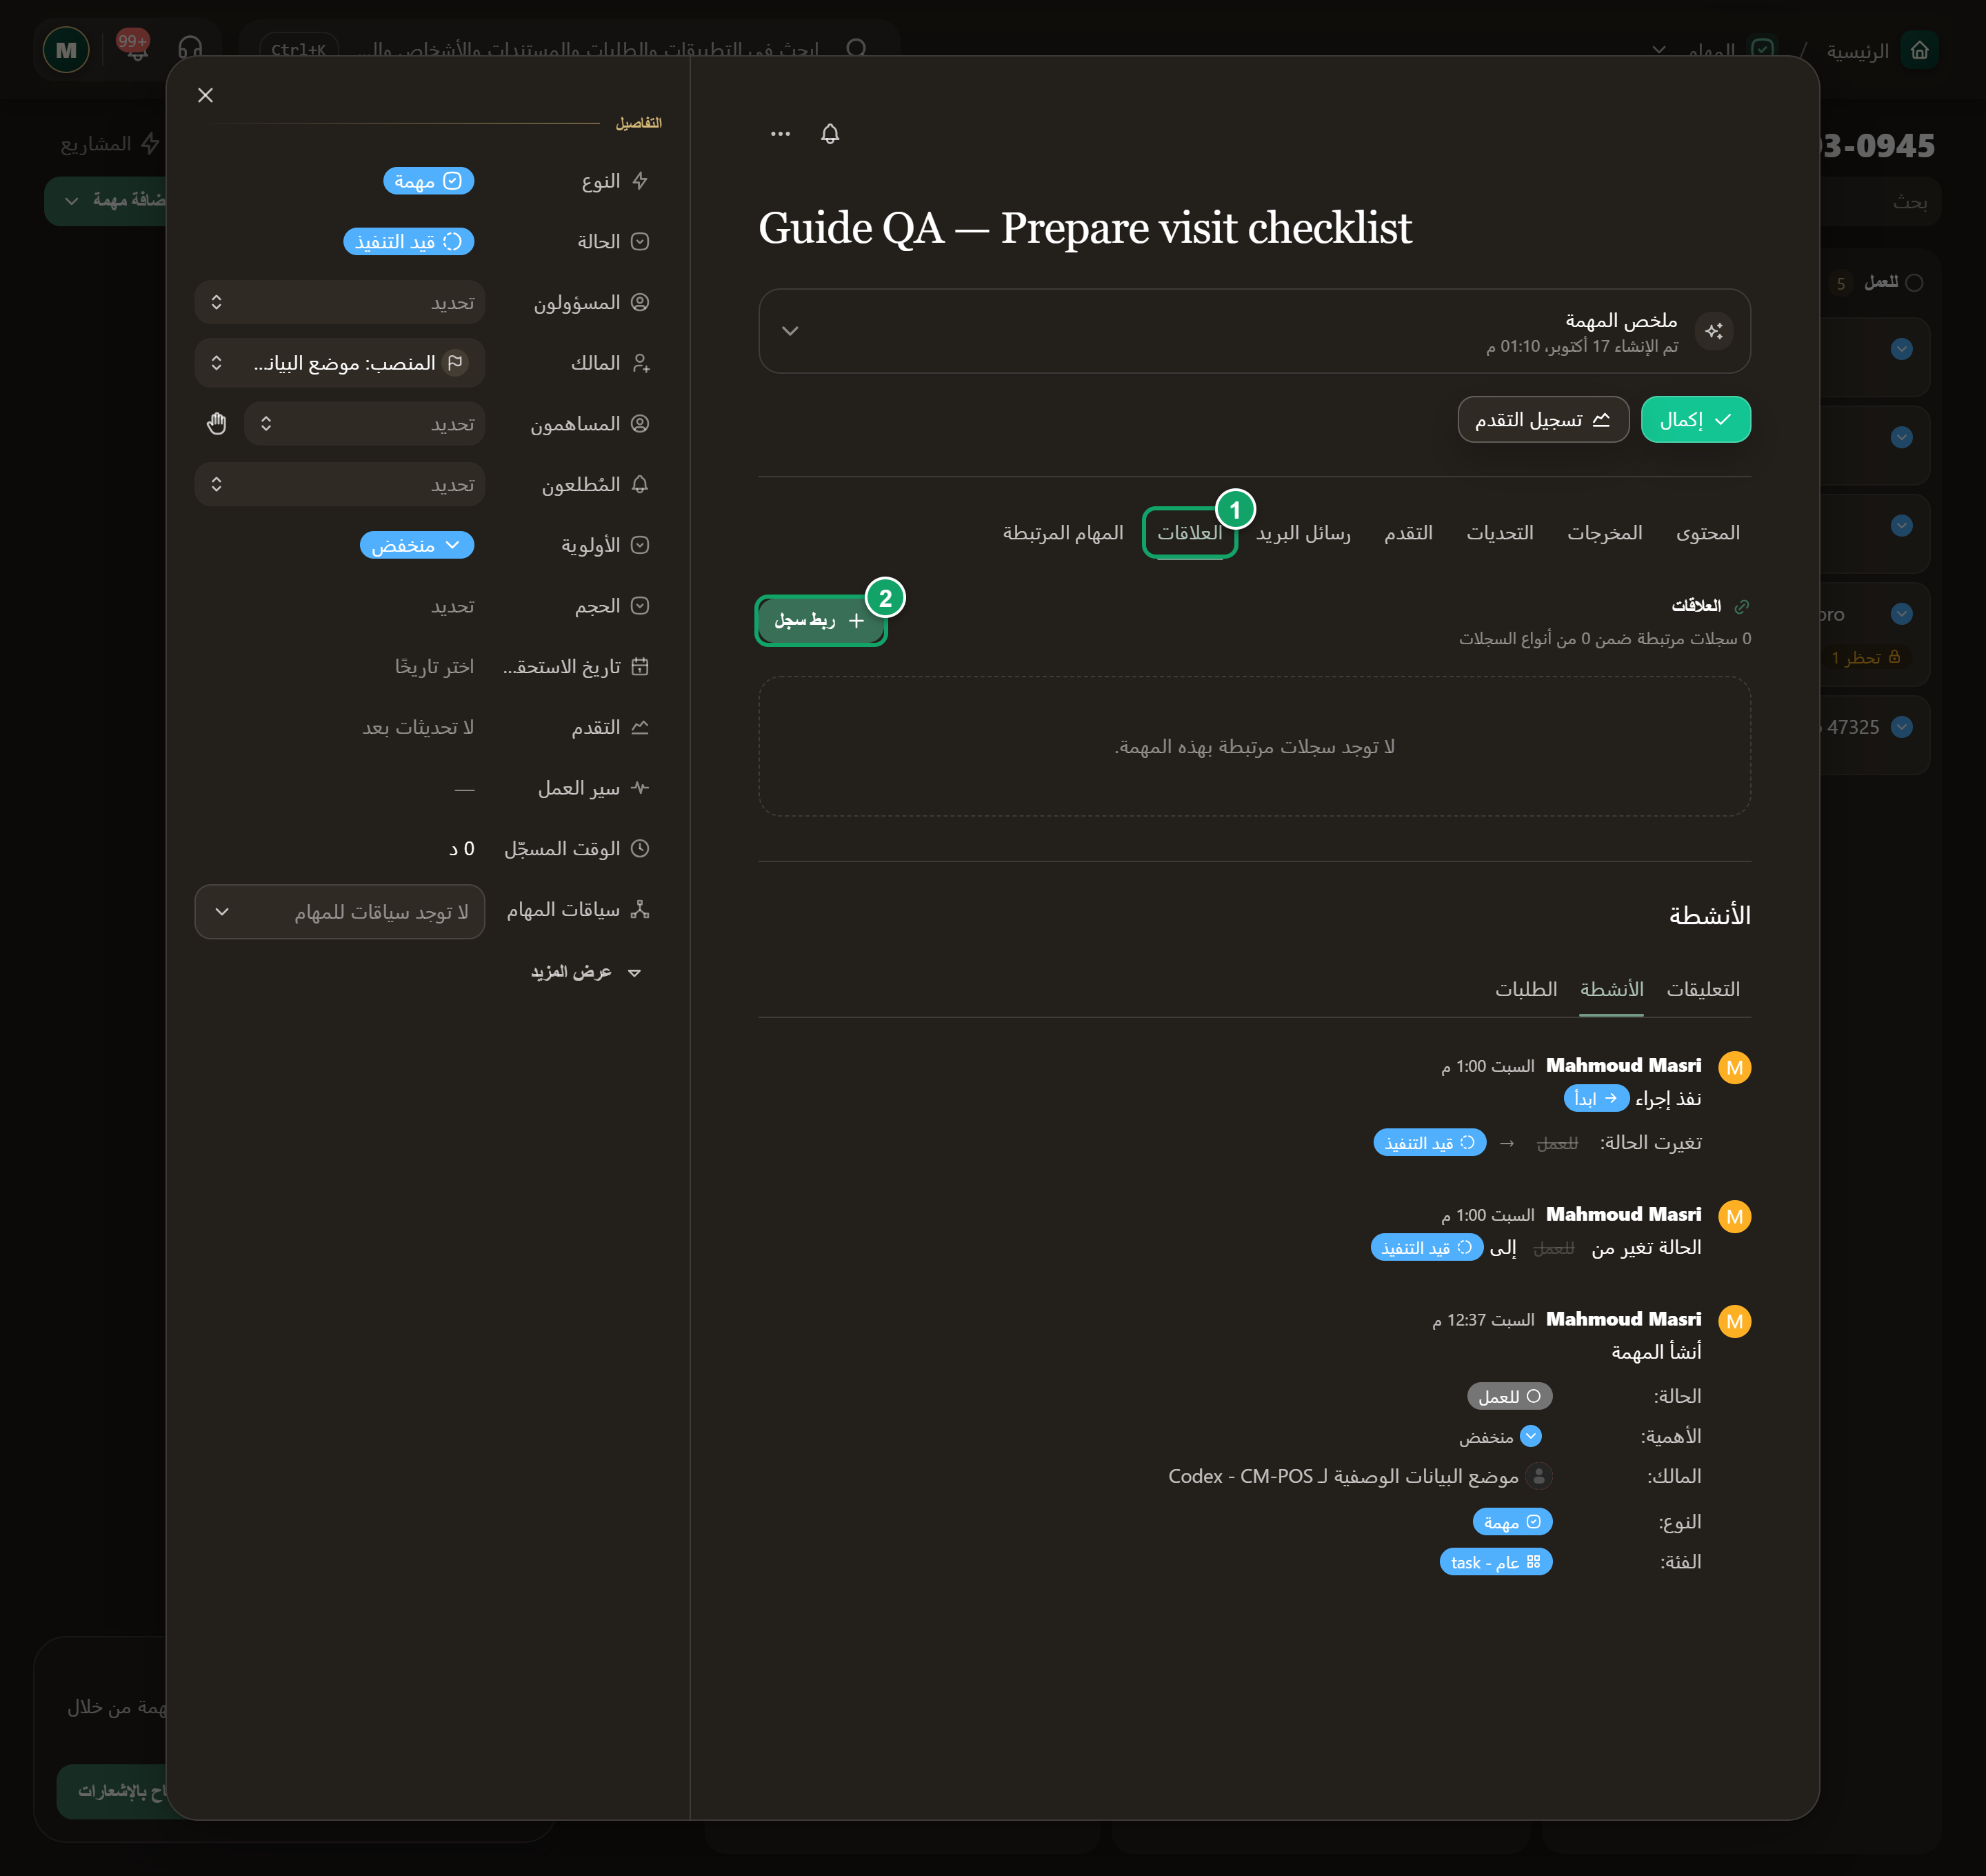
\includegraphics[width=0.95\linewidth,height=0.72\textheight,keepaspectratio]{figures/screens/ch04-records-ar.png}
\caption{علاقات السجلات}
\label{fig:tasks-relationships-records}
\shotnote{يربط تبويب «العلاقات» المهمة بسجلات من خارج المهام، كسجل يمثل موضوعها أو يثبت إنجازها، ويعرض عدد السجلات المرتبطة. ويبدأ الربط بزر «ربط سجل» واختيار معنى العلاقة من الأنواع المسموحة. ولا يمنح الرابط صلاحية فتح السجل لمن لا يملكها، والقائمة فارغة في هذه المهمة التجريبية. ① تبويب «العلاقات». ② «ربط سجل»: يربط المهمة بسجل آخر في كيان.}
\end{figure}

\begin{figure}[H]
\centering
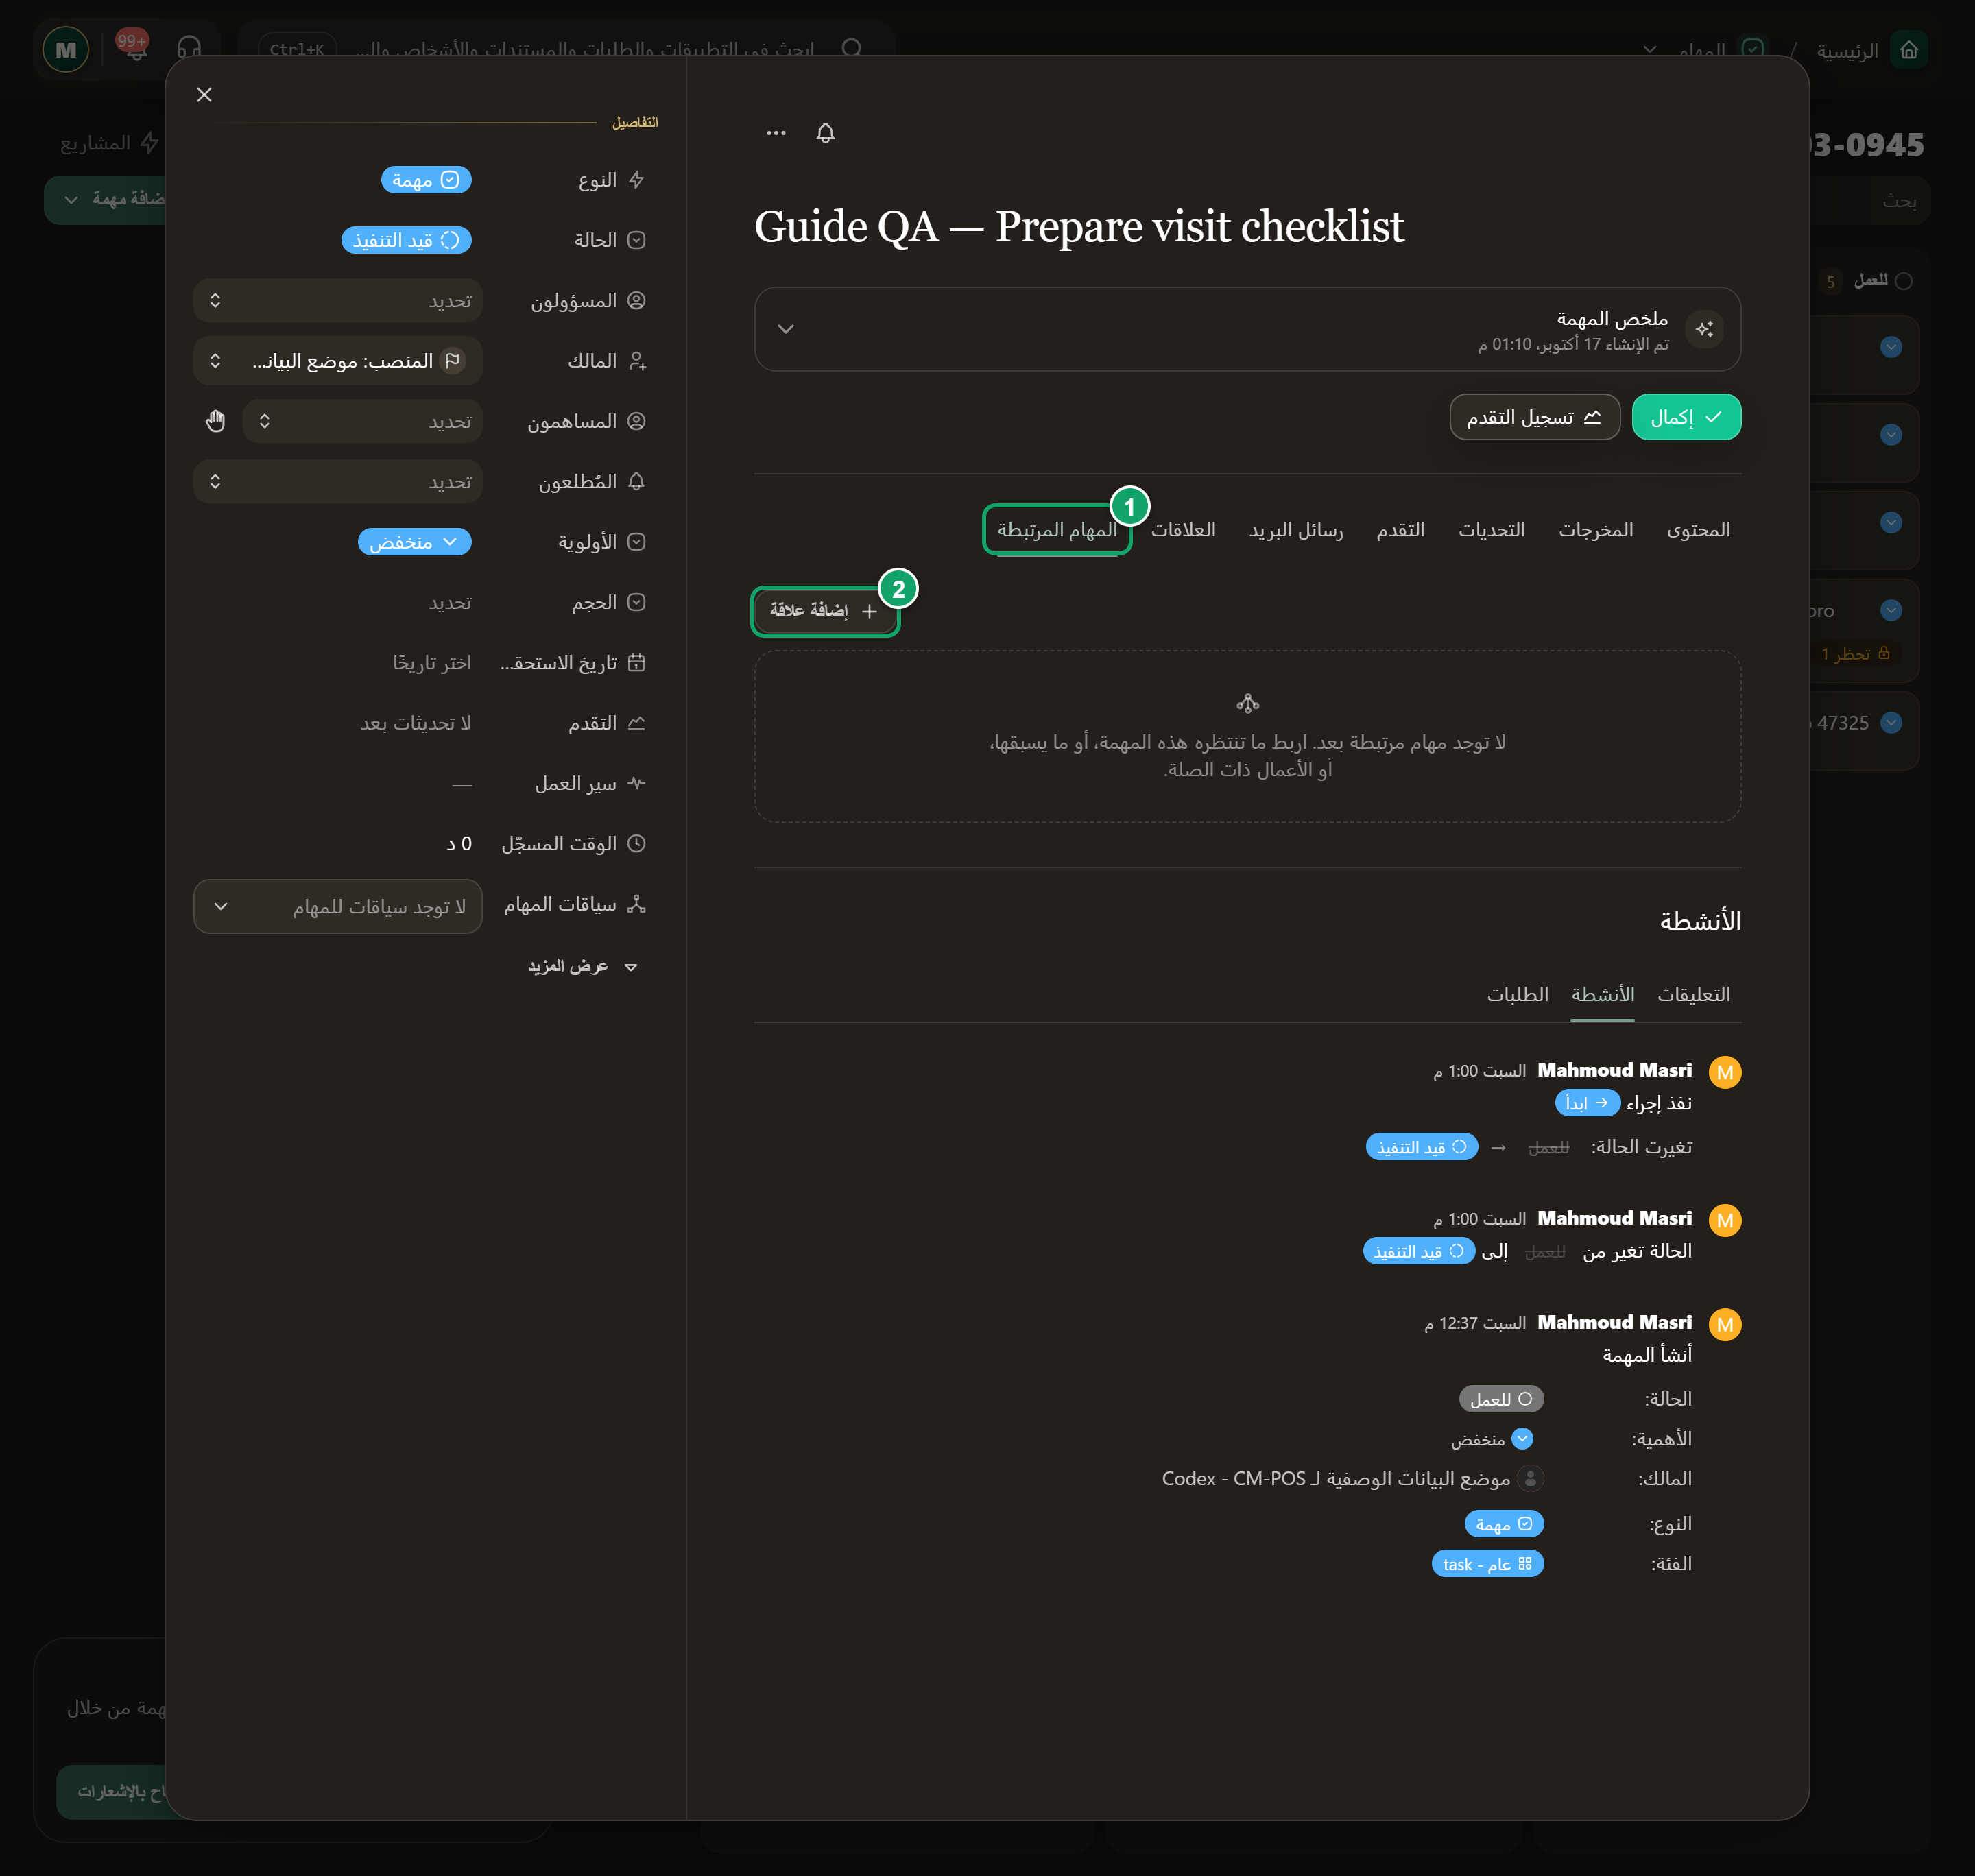
\includegraphics[width=0.95\linewidth,height=0.72\textheight,keepaspectratio]{figures/screens/ch04-relations-ar.png}
\caption{المهام المرتبطة}
\label{fig:tasks-relationships-relations}
\shotnote{يعرض تبويب «المهام المرتبطة» صلة المهمة بمهام أخرى: ما تنتظره، وما يسبقها، وما يتصل بها، ويُضاف الرابط من «إضافة علاقة». وتؤثر بعض هذه العلاقات في ترتيب العمل، لذلك تحقق من اتجاه علاقة الحجب قبل حفظها. ولا توجد علاقات بعد في هذه المهمة التجريبية. ① تبويب «المهام المرتبطة». ② «إضافة علاقة»: يربط المهمة بمهمة أخرى، مثل مهمة تحظرها.}
\end{figure}

\begin{figure}[H]
\centering
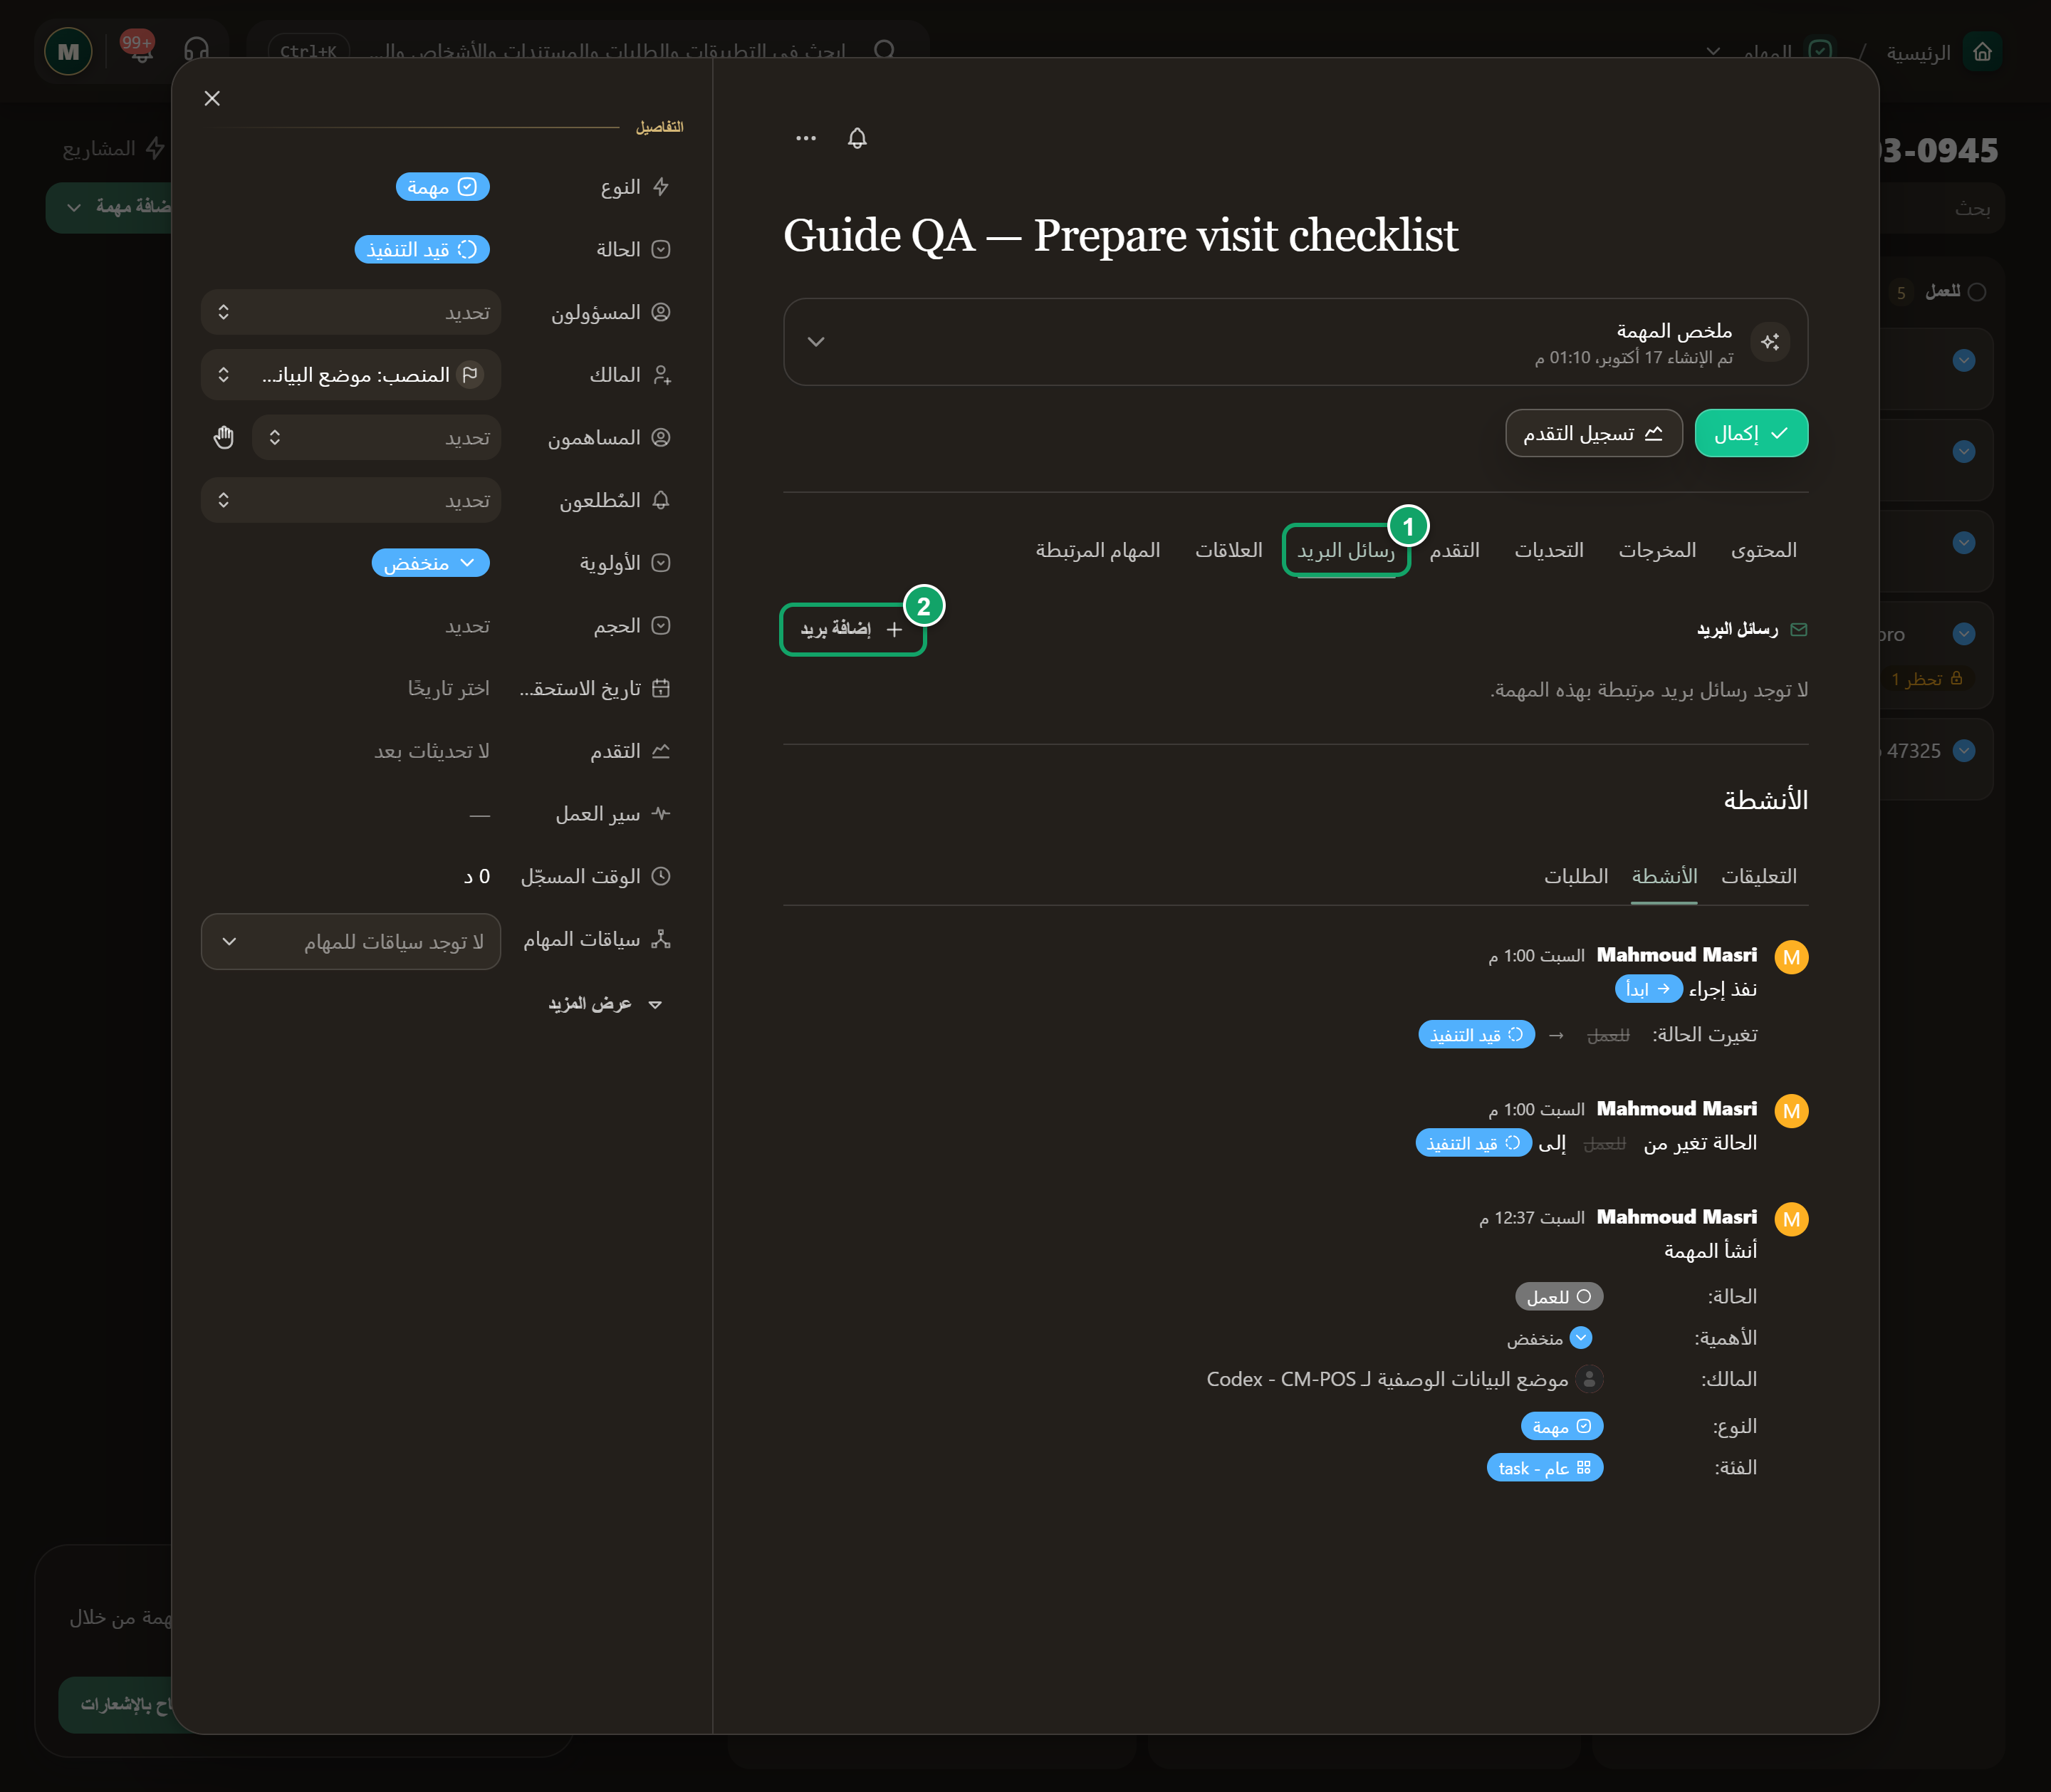
\includegraphics[width=0.95\linewidth,height=0.72\textheight,keepaspectratio]{figures/screens/ch04-emails-ar.png}
\caption{البريد المرتبط}
\label{fig:tasks-relationships-emails}
\shotnote{يجمع تبويب «رسائل البريد» المراسلات المرتبطة بالمهمة، ويربط زر «إضافة بريد» رسالة جديدة بها، فيجد الفريق سياق الطلب الأصلي دون البحث في البريد. والقائمة فارغة هنا، فلا تفترض أن رسالة ما مرتبطة بالمهمة ما لم تظهر في هذا التبويب. ① تبويب «رسائل البريد». ② «إضافة بريد»: يربط رسالة بريد بالمهمة.}
\end{figure}

\begin{table}[H]
\centering
\caption{ما الذي تجده هنا؟}
\label{tab:tasks-relationships-data}
\begin{tabularx}{\linewidth}{R{3.6cm} Y}
\rcHeaderRow
\thh{القسم} & \thh{المحتوى والإجراء}\\
العلاقات & معنى الرابط ونوع السجل والسجل نفسه، مع ملاحظة عند الحاجة. وقد يشترط نوع المهمة روابط معينة عند الإنشاء أو الإكمال.\\
المهام المرتبطة & علاقات بين مهمتين، مثل الحجب أو المهمة الرئيسية والفرعية، بحسب الأنواع المفعّلة. ويمكن البحث في مجموعات أخرى متاحة لك.\\
البريد والسياقات & يقدّم البريد سياق المراسلة، وتربط سياقات المشاريع والتخطيط التنفيذ بالعمل الأكبر، بحسب الخيارات المتاحة.\\
\end{tabularx}
\end{table}

\begin{figure}[H]
\centering
\begin{tikzpicture}[node distance=0.5cm]
\node[stepBox] (a) {\RL{تحديد معنى العلاقة}};
\node[stepBox,below=of a] (b) {\RL{اختيار السجل أو المهمة}};
\node[stepBox,below=of b] (c) {\RL{تحقق من الرابط والاتجاه}};
\draw[flowsTo] (a) -- (b);
\draw[flowsTo] (b) -- (c);
\end{tikzpicture}
\rclegend
\caption{خطوات الاستخدام}
\label{fig:tasks-relationships-flow}
\shotnote{يبدأ الربط الصحيح من المعنى لا من السجل: حدّد أولاً هل الرابط مصدر أو دليل أو تبعية، ثم ابحث عن السجل أو المهمة المناسبة، وتحقق أخيراً من الهدف والاتجاه. فالعلاقة المعكوسة قد تجعل المهمة الخطأ هي التي تنتظر غيرها.}
\end{figure}

\subsection{خطوات العمل والتحقق}
\begin{enumerate}
\item في «العلاقات» اضغط «ربط سجل»، ثم اختر معنى العلاقة ونوع السجل، وابحث عن السجل الصحيح وحدده واحفظ.
\item في «المهام المرتبطة» اضغط «إضافة علاقة»، وحدد النوع والمهمة، وراجع اتجاه العلاقة قبل تأكيدها.
\item افتح الرابط المحفوظ وتأكد أنه يشير إلى السجل المقصود، وراجع المهام الحاجبة قبل محاولة الإكمال.
\end{enumerate}

\textbf{تحقق ومعالجة المشكلة:} إذا لم يظهر السجل، فراجع النوع ونص البحث والصلاحيات. ولا تحذف تبعية صحيحة لتتجاوز منع الإكمال، ولا تعدّ الرابط موافقة أو تحديثاً تلقائياً للسجل.

\clearpage
\section{المهام الكبرى}
\label{sec:tasks-feature-epics}

تجمع المهمة الكبرى عدة مهام تخدم نتيجة أوسع. ويظهر تبويبها في الواجهة العربية باسم «المشاريع»، وهو غير تطبيق المشاريع والتخطيط. استخدمها عندما يحتاج العمل إلى تقسيم مع بقاء الهدف واضحاً في مكان واحد.

\textbf{المسار ومن يستخدمه:} «المهام» ← مجموعة ← تبويب «المشاريع». يستخدمها المسؤول عن مجموعة من الأعمال المترابطة.

\begin{rcnote}[مثال: شركة الأفق]
تنظّم سارة «تجهيز زيارة فرع حلب» مهمةً كبرى، وتربط بها مهمة عمر لتجهيز القائمة ومهمة أخرى لتأكيد الموعد.
\end{rcnote}

\begin{figure}[H]
\centering
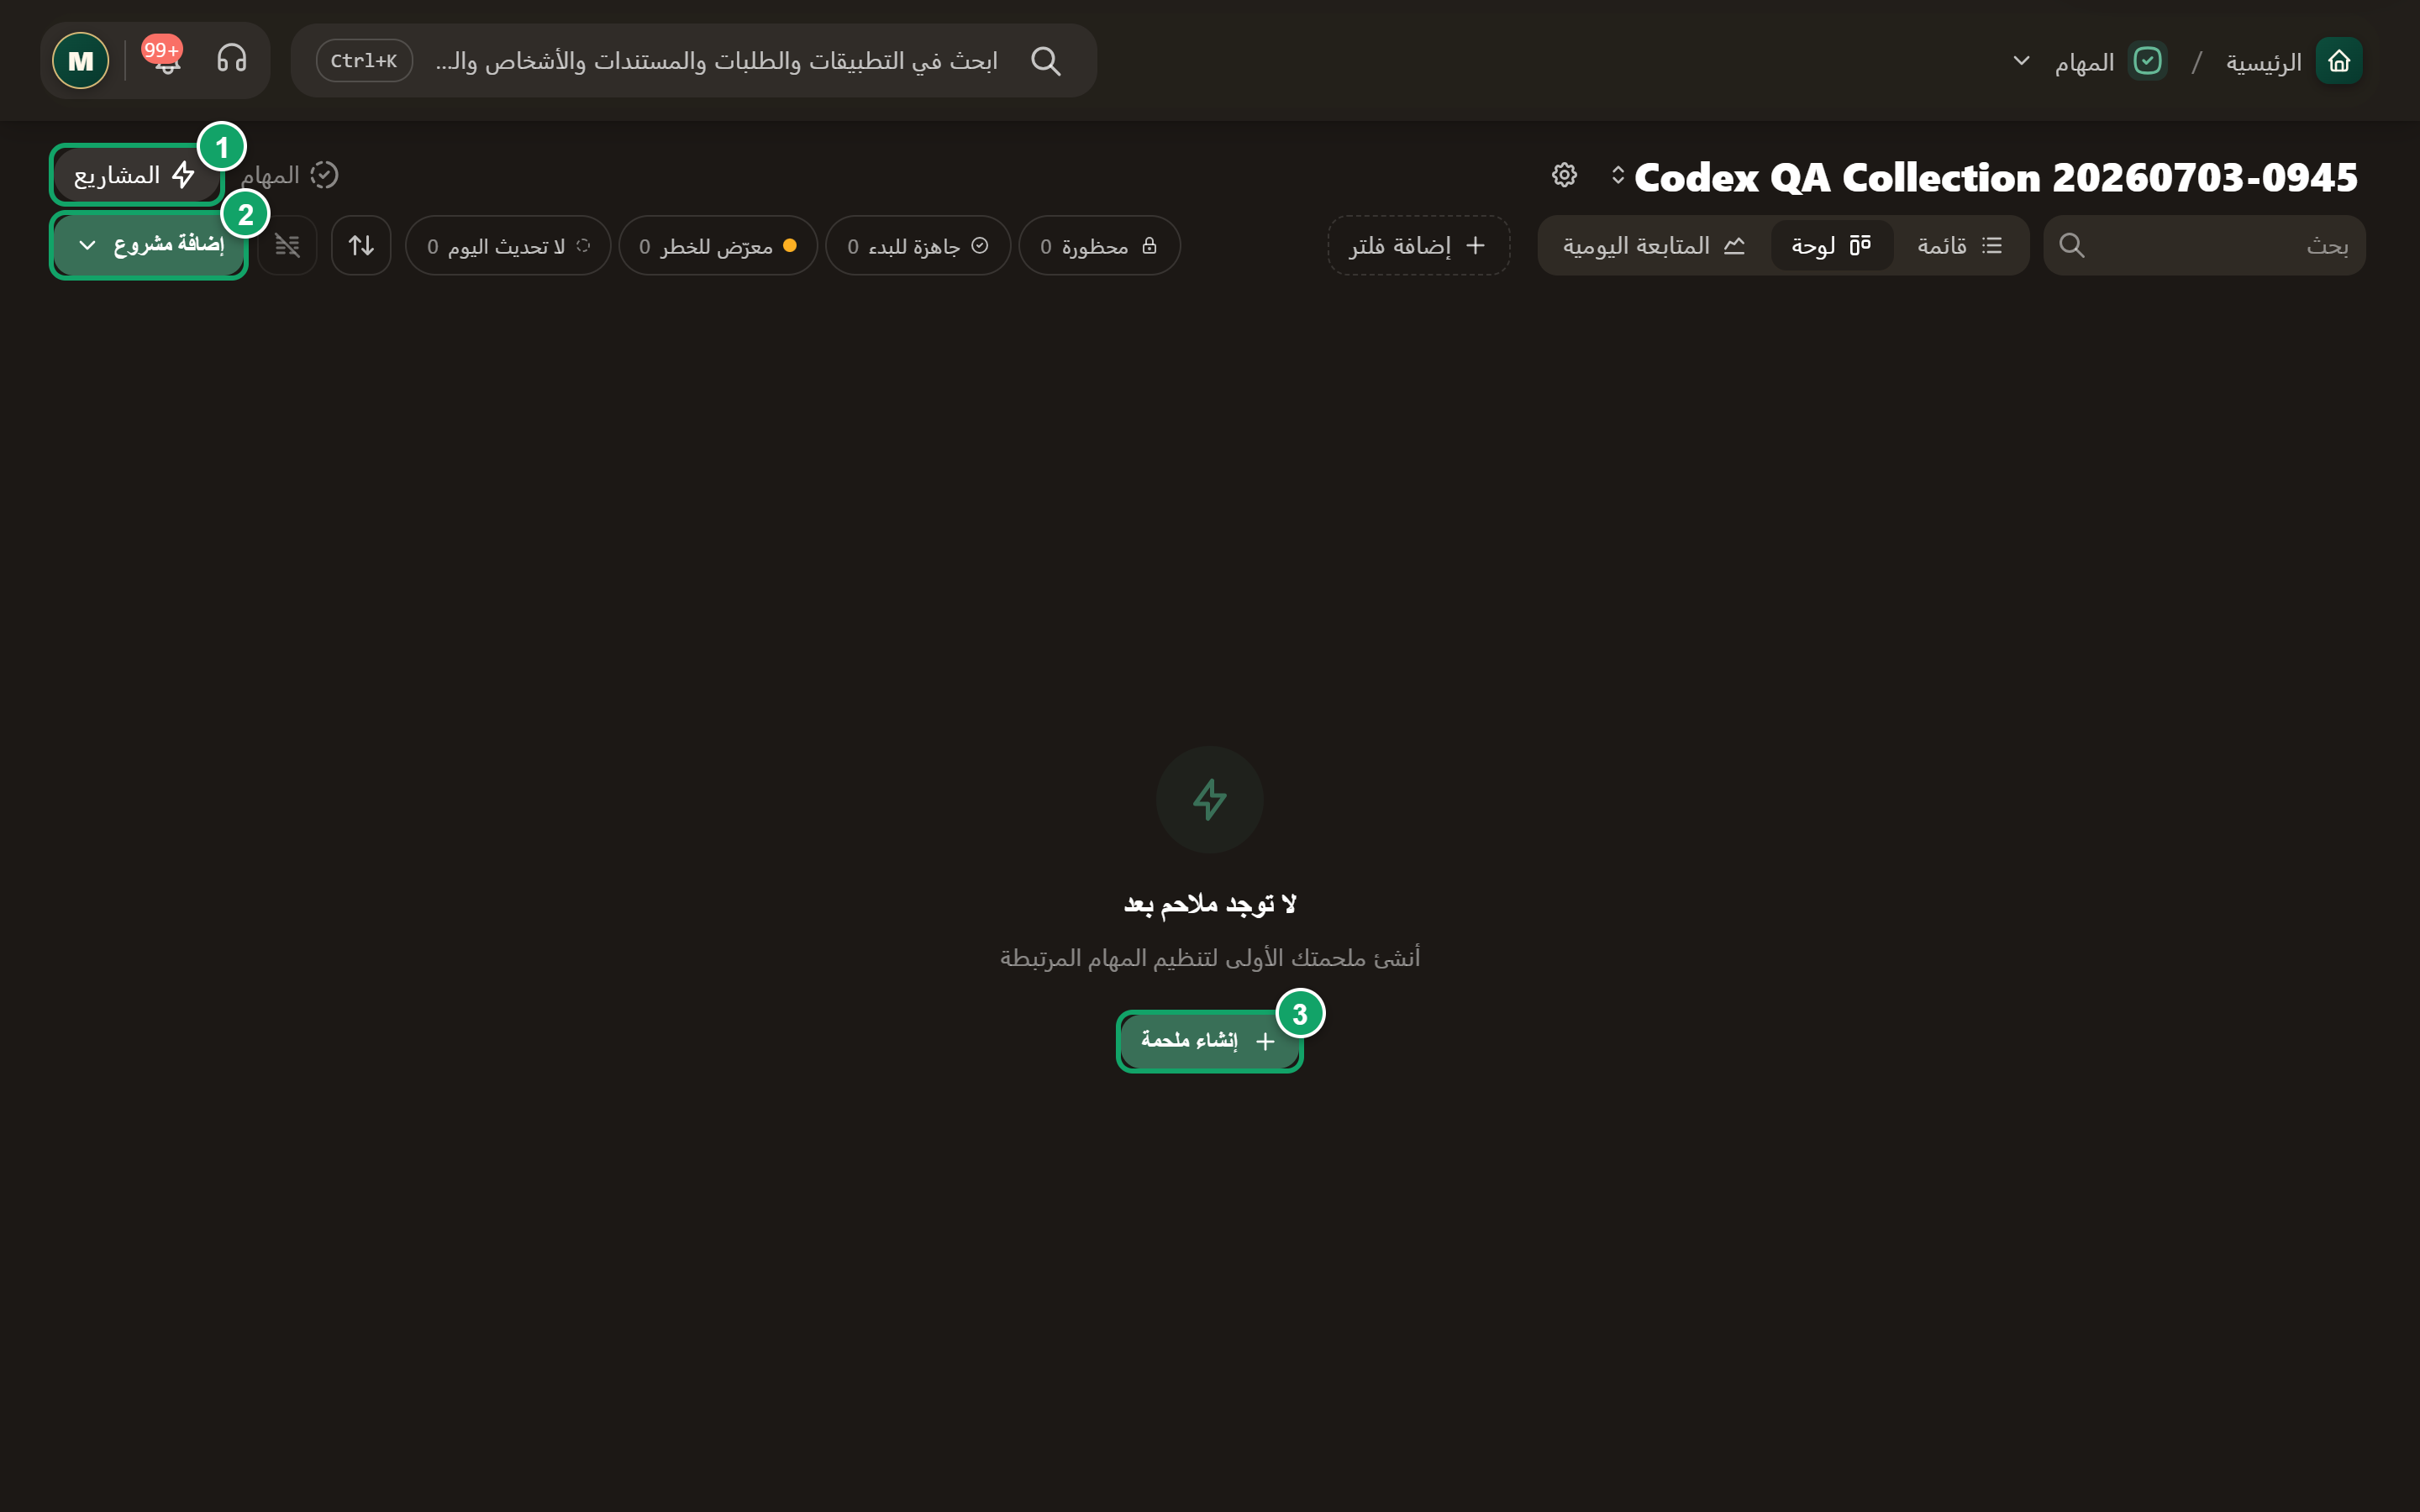
\includegraphics[width=0.95\linewidth,height=0.72\textheight,keepaspectratio]{figures/screens/ch04-epics-ar.png}
\caption{تبويب المهام الكبرى}
\label{fig:tasks-epics-epics}
\shotnote{يعرض تبويب «المشاريع» داخل المجموعة المهام الكبرى بأدوات العرض نفسها التي تستخدمها مع المهام، ويضيف زر «إضافة مشروع». والتبويب فارغ في مجموعة الاختبار، وتسمي رسالته المهمة الكبرى «ملحمة»، وهي تسمية أخرى للشيء نفسه. ولا يفتح هذا التبويب تطبيق المشاريع والتخطيط. ① التبديل إلى عرض «المشاريع»، أي المهام الكبرى في المجموعة. ② «إضافة مشروع»: ينشئ مهمة كبرى جديدة. ③ «إنشاء ملحمة»: يفعل الشيء نفسه عندما لا توجد مهام كبرى بعد.}
\end{figure}

\begin{table}[H]
\centering
\caption{ما الذي تجده هنا؟}
\label{tab:tasks-epics-data}
\begin{tabularx}{\linewidth}{R{3.6cm} Y}
\rcHeaderRow
\thh{القسم} & \thh{المحتوى والإجراء}\\
التفاصيل والمحتوى & العنوان والنوع والحالة والمسؤوليات والموعد والمحتوى، بحسب نوع المهمة الكبرى.\\
المهام التابعة & إنشاء مهمة أو ربط مهمة موجودة، وفتحها أو إزالة ربطها بحسب الصلاحية. وإزالة الربط لا تحذف المهمة.\\
\end{tabularx}
\end{table}

\begin{figure}[H]
\centering
\begin{tikzpicture}[node distance=0.5cm]
\node[stepBox] (a) {\RL{تحديد النتيجة العامة}};
\node[stepBox,below=of a] (b) {\RL{ربط المهام}};
\node[stepBox,below=of b] (c) {\RL{متابعة كل نتيجة}};
\draw[flowsTo] (a) -- (b);
\draw[flowsTo] (b) -- (c);
\end{tikzpicture}
\rclegend
\caption{خطوات الاستخدام}
\label{fig:tasks-epics-flow}
\shotnote{يبيّن المخطط أن المهمة الكبرى إطار للمتابعة لا بديل عن المهام: حدّد النتيجة العامة، ثم اربط بها المهام التي تحققها، وتابع نتيجة كل مهمة على حدة. وبذلك تقيّم العمل كله من نتائج أجزائه، لا من حالة المهمة الكبرى وحدها.}
\end{figure}

\subsection{خطوات العمل والتحقق}
\begin{enumerate}
\item افتح تبويب «المشاريع»، واضغط «إضافة مشروع» واختر النوع المتاح، ثم اكتب النتيجة العامة والمسؤولية وأنشئ السجل.
\item داخل المهمة الكبرى أضف مهمة أو اربط مهمة موجودة، واختر عنوان العمل الصحيح ثم أكّد الربط.
\item افتح المهمة التابعة وتحقق من الربط، وتابع حالة كل مهمة قبل تحديث المهمة الكبرى.
\end{enumerate}

\textbf{تحقق ومعالجة المشكلة:} لا تفترض أن إغلاق المهمة الكبرى يغلق المهام التابعة أو أي مشروع مرتبط، بل راجع النتائج والحالات كلاً على حدة.

\clearpage
\section{اقتراحات الذكاء الاصطناعي}
\label{sec:tasks-feature-suggestions}

المقترح عمل مستخرج من رسائل البريد، ويحتاج إلى مراجعة قبل أن يصبح مهمة فعلية. راجع مصدره والمسؤولية والموعد قبل قبوله.

\textbf{المسار ومن يستخدمه:} «المهام» ← بطاقة «اقتراحات الذكاء الاصطناعي» عند تفعيلها. يستخدمها المراجع المخوّل.

\begin{rcnote}[مثال: شركة الأفق]
تراجع سارة مقترحاً لتأكيد زيارة الأفق، فتختار مجموعة «زيارات الأفق» عند القبول، ثم تصحح الموعد في المهمة الناتجة.
\end{rcnote}

\begin{figure}[H]
\centering
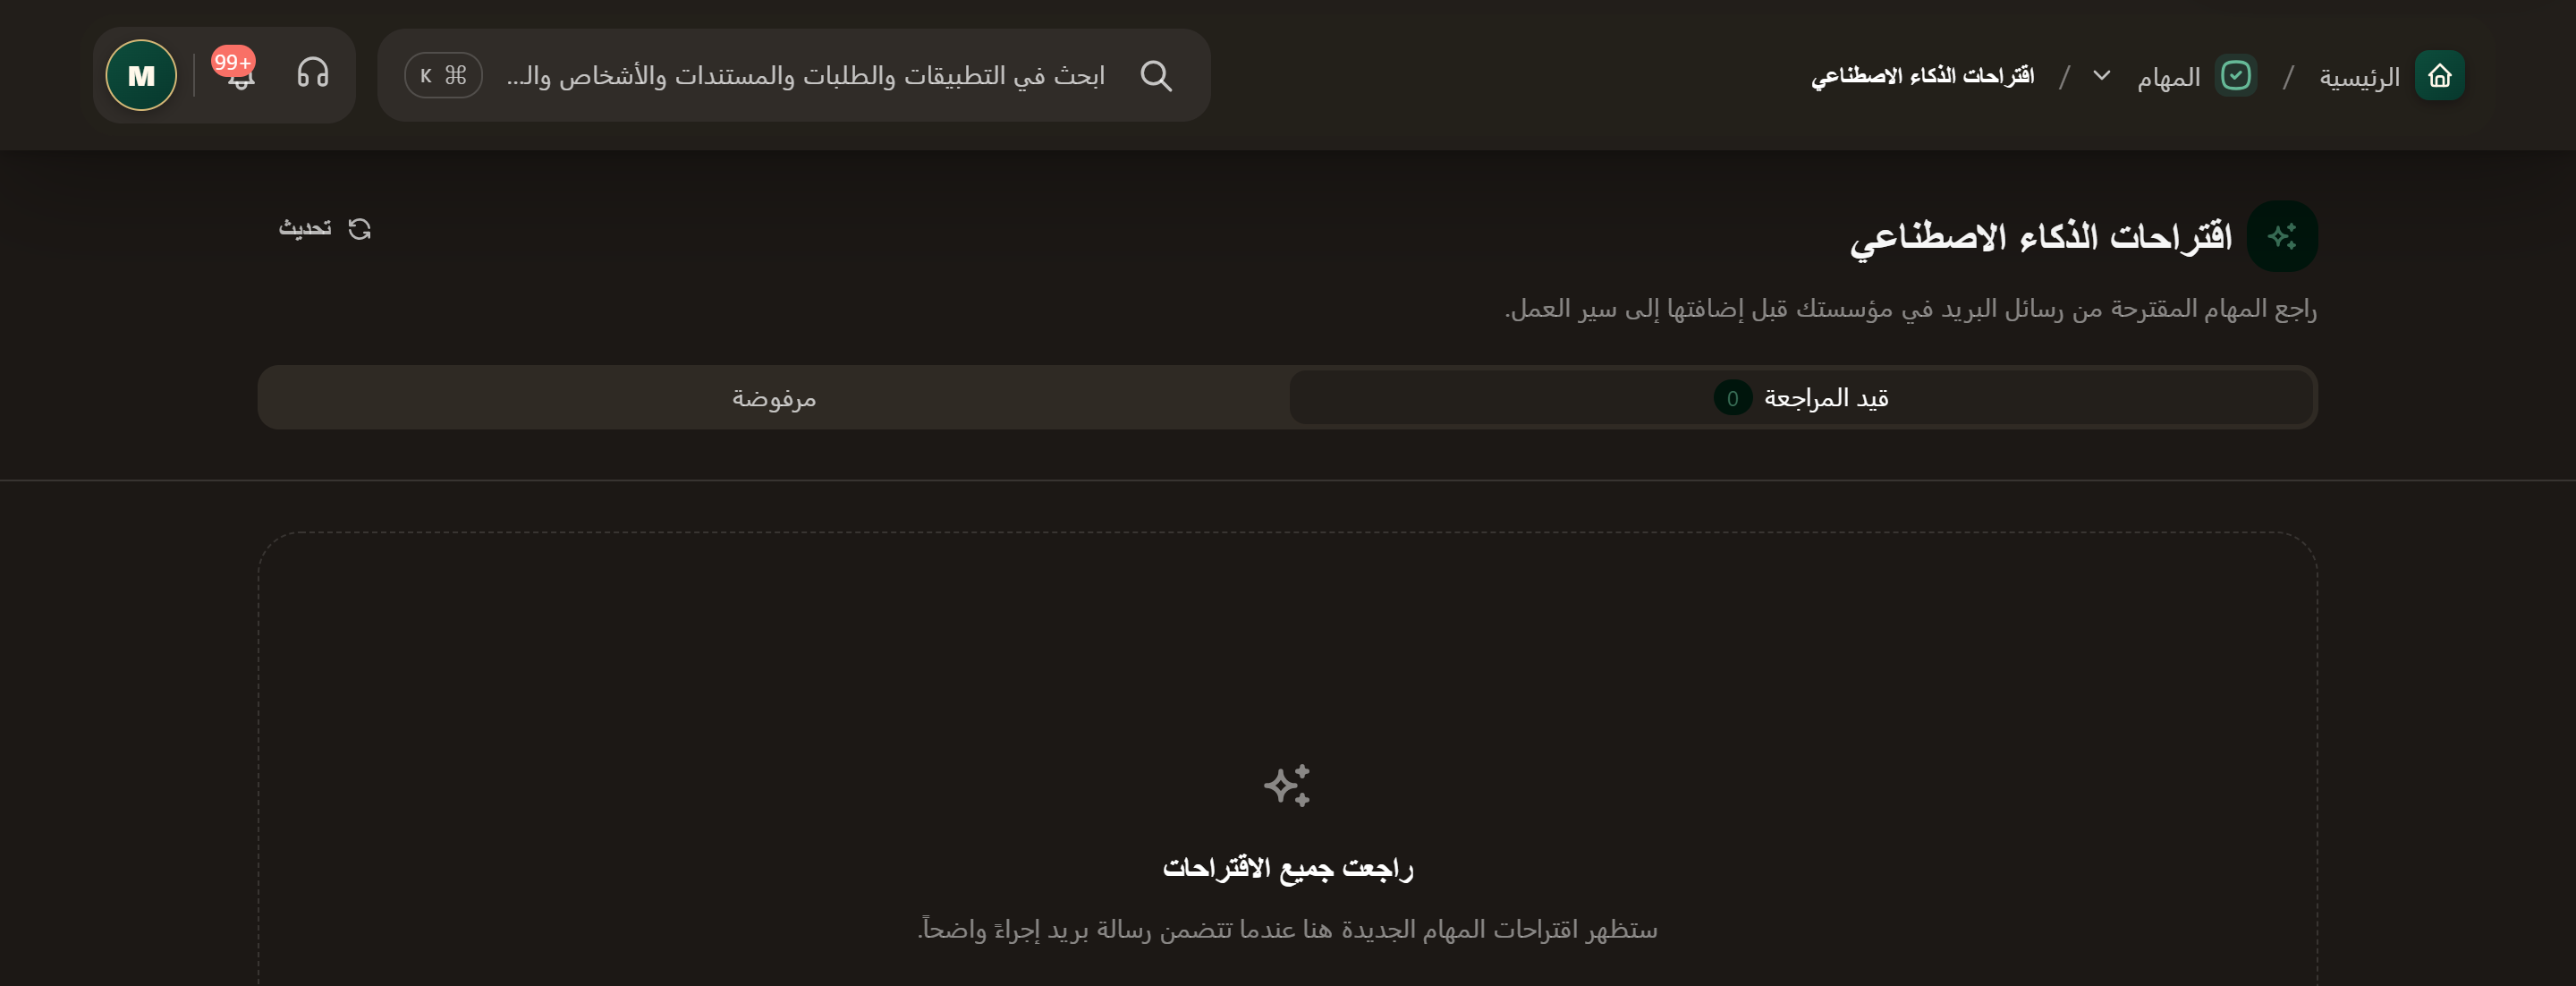
\includegraphics[width=0.95\linewidth,height=0.72\textheight,keepaspectratio]{figures/screens/ch04-suggestions-ar.png}
\caption{قائمة المقترحات}
\label{fig:tasks-suggestions-suggestions}
\shotnote{تجمع هذه الصفحة المهام المقترحة من رسائل البريد في تبويبين: «قيد المراجعة» لما ينتظر قرارك، و«مرفوضة» لما استبعدته، فلا يدخل المقترح سير العمل حتى يقبله مراجع. والقائمة فارغة في test2 وقت الالتقاط، لذلك لم يُختبر القبول هنا. ① «قيد المراجعة»: الاقتراحات التي تنتظر قرارك. ② «مرفوضة». ③ «تحديث».}
\end{figure}

\begin{table}[H]
\centering
\caption{ما الذي تجده هنا؟}
\label{tab:tasks-suggestions-data}
\begin{tabularx}{\linewidth}{R{3.6cm} Y}
\rcHeaderRow
\thh{القسم} & \thh{المحتوى والإجراء}\\
الحالة والمصدر & صفِّ المقترحات بحالتها، وافتح تفاصيلها، وراجع البريد الذي استندت إليه.\\
القبول أو الرفض & يتطلب القبول مجموعة ونوعاً مسموحين وبيانات صحيحة، أما الرفض فلا يعني إكمال مهمة.\\
\end{tabularx}
\end{table}

\begin{figure}[H]
\centering
\begin{tikzpicture}[node distance=0.5cm]
\node[stepBox] (a) {\RL{قراءة المصدر}};
\node[stepBox,below=of a] (b) {\RL{مراجعة المقترح}};
\node[stepBox,below=of b] (c) {\RL{قبول ثم تحقق}};
\draw[flowsTo] (a) -- (b);
\draw[flowsTo] (b) -- (c);
\end{tikzpicture}
\rclegend
\caption{خطوات الاستخدام}
\label{fig:tasks-suggestions-flow}
\shotnote{يضع المخطط قراءة المصدر قبل أي قرار، لأن رسالة البريد هي التي تفسر سبب المقترح ومن طلبه. ثم تأتي مراجعة تفاصيله، وبعدها القبول والتحقق من المهمة الناتجة؛ إذ لا يتحول المقترح إلى مهمة إلا بقرار من المراجع.}
\end{figure}

\subsection{خطوات العمل والتحقق}
\begin{enumerate}
\item افتح «اقتراحات الذكاء الاصطناعي» واختر «قيد المراجعة»، ثم افتح مقترحاً إن وُجد واقرأ مصدره.
\item راجع المقترح ومصدره قبل القبول، ثم اختر نوع المهمة ومجموعة واحدة على الأقل وأكّد القبول، أو ارفض المقترح غير المناسب.
\item بعد القبول افتح المهمة الناتجة، وصحّح العنوان والأشخاص والتاريخ عند الحاجة، ثم تحقق من الحفظ. أما إذا كانت القائمة فارغة فلا يوجد ما تقبله.
\end{enumerate}

\textbf{تحقق ومعالجة المشكلة:} إذا غاب النوع المطلوب، فراجع صلاحية إنشائه وقيود المجموعة. وتذكّر أن المقترح وحده ليس تكليفاً مؤكداً.

\clearpage
\section{التكليفات}
\label{sec:tasks-feature-assignments}

تعرض «التكليفات» النماذج المطلوب منك تعبئتها والعمل المرتبط بها، فتبدأ من التكليف وتعود إليه لمراجعة نتيجته. أما تصميم النماذج وإدارة خطط التكليف فلهما أدوات أخرى.

\textbf{المسار ومن يستخدمه:} «المهام» ← «التكليفات». يستخدمها الشخص المكلّف بتعبئة نموذج.

\begin{rcnote}[مثال: شركة الأفق]
يفتح عمر تكليف نموذج زيارة الأفق، فيكمل حقوله ثم يرسله، وتراجع سارة النتيجة وفق مسار النموذج.
\end{rcnote}

\begin{figure}[H]
\centering

\includegraphics[width=0.95\linewidth,height=0.72\textheight,keepaspectratio]{figures/screens/ch04-assignments-ar.png}
\caption{قائمة التكليفات}
\label{fig:tasks-assignments-assignments}
\shotnote{تجمع الصفحة العمل المطلوب منك في «المطلوب مني» وترتبه حسب الموعد، ولكل تكليف زر يناسب حالته لبدء التعبئة أو متابعتها. ويُظهر التبديل بين «مفتوحة» و«منجزة» العمل الحالي أو السابق، أما تبويب «الخطط» فيخص متابعة توزيع العمل. وتظهر بطاقة «عمل اليوم» عندما يتوفر تكليف يمكن تنزيله للعمل دون اتصال. ① عنوان صفحة «التكليفات». ② «المطلوب مني»: النماذج المسندة إليك وعددها.}
\end{figure}

\begin{table}[H]
\centering
\caption{ما الذي تجده هنا؟}
\label{tab:tasks-assignments-data}
\begin{tabularx}{\linewidth}{R{3.6cm} Y}
\rcHeaderRow
\thh{القسم} & \thh{المحتوى والإجراء}\\
بطاقة التكليف & عنوان النموذج والموعد والحالة والنتيجة المتاحة.\\
الإجراءات & البدء أو المتابعة أو العرض، واستلام التكليف أو «اعتذار» حيث تسمح الخطة. وقد يطلب إجراء «نتيجة دون إجابة» سبباً أو صورة أو موقعاً قبل الإغلاق.\\
المطلوب مني والخطط & يعرض «المطلوب مني» تكليفاتك مرتبة حسب الموعد، ويفتح «الخطط» متابعة توزيع العمل لمن يملك صلاحيتها.\\
الحزم والعمل الميداني & تجمع الحزمة نماذج مترابطة وتعرض الوحدة التالية. ويظهر تنزيل العمل دون اتصال و«صندوق الإرسال» للعمل المؤهل، فتحقق من المزامنة عند عودة الاتصال.\\
الغياب والترتيب & يسجّل «غائب حتى…» فترة عدم توفرك، وقد يتاح ترتيب المجموعات أو عرض الخريطة بحسب بيانات العمل.\\
\end{tabularx}
\end{table}

\begin{figure}[H]
\centering
\begin{tikzpicture}[node distance=0.5cm]
\node[stepBox] (a) {\RL{فتح التكليف}};
\node[stepBox,below=of a] (b) {\RL{تعبئة وإرسال}};
\node[stepBox,below=of b] (c) {\RL{مراجعة النتيجة}};
\draw[flowsTo] (a) -- (b);
\draw[flowsTo] (b) -- (c);
\end{tikzpicture}
\rclegend
\caption{خطوات الاستخدام}
\label{fig:tasks-assignments-flow}
\shotnote{يربط المخطط بداية العمل بنهايته: افتح التكليف نفسه لتصل إلى النموذج الصحيح، ثم عبّئه وأرسله، وبعدها راجع نتيجته. فوجود مسودة لا يعني أن التكليف أُنجز؛ العبرة بالإرسال وبالنتيجة التي تظهر بعده.}
\end{figure}

\subsection{خطوات العمل والتحقق}
\begin{enumerate}
\item افتح «التكليفات» واختر التكليف المقصود، وإن كان متاحاً للاستلام فاستلمه قبل البدء.
\item اختر البدء أو المتابعة، وأكمل حقول النموذج، ثم استخدم إجراء الإرسال الذي يقدمه النموذج.
\item ارجع إلى «التكليفات» واعرض «منجزة» عند الحاجة، ثم اضغط «عرض» للتحقق. أما «نتيجة دون إجابة» فإجراء مستقل يغلق التكليف عند السماح به، وليس زراً لعرض النتيجة.
\end{enumerate}

\textbf{تحقق ومعالجة المشكلة:} الحفظ كمسودة ليس إرسالاً. وإذا لم يظهر تكليف متوقع، فراجع المستلم والخطة والصلاحية مع المسؤول.

\clearpage
\section{إعدادات المهام}
\label{sec:tasks-feature-settings}

تحدد إعدادات المهام أنواع العمل وفئاته والعلاقات المتاحة. وهي تهيئة يتولاها المسؤول، أما الموظف فيستخدم عادةً الأنواع الجاهزة.

\textbf{المسار ومن يستخدمه:} «أدوات البناء» ← «إعدادات المهام». يستخدمها المسؤول المخوّل.

\begin{rcnote}[مثال: شركة الأفق]
تراجع سارة مع المسؤول نوع مهمة الزيارة: الفئة الافتراضية، ومسار الحالات، وهل يلزم تحديث التقدم. ثم تستخدم هذا النوع في مهام الأفق.
\end{rcnote}

\begin{figure}[H]
\centering
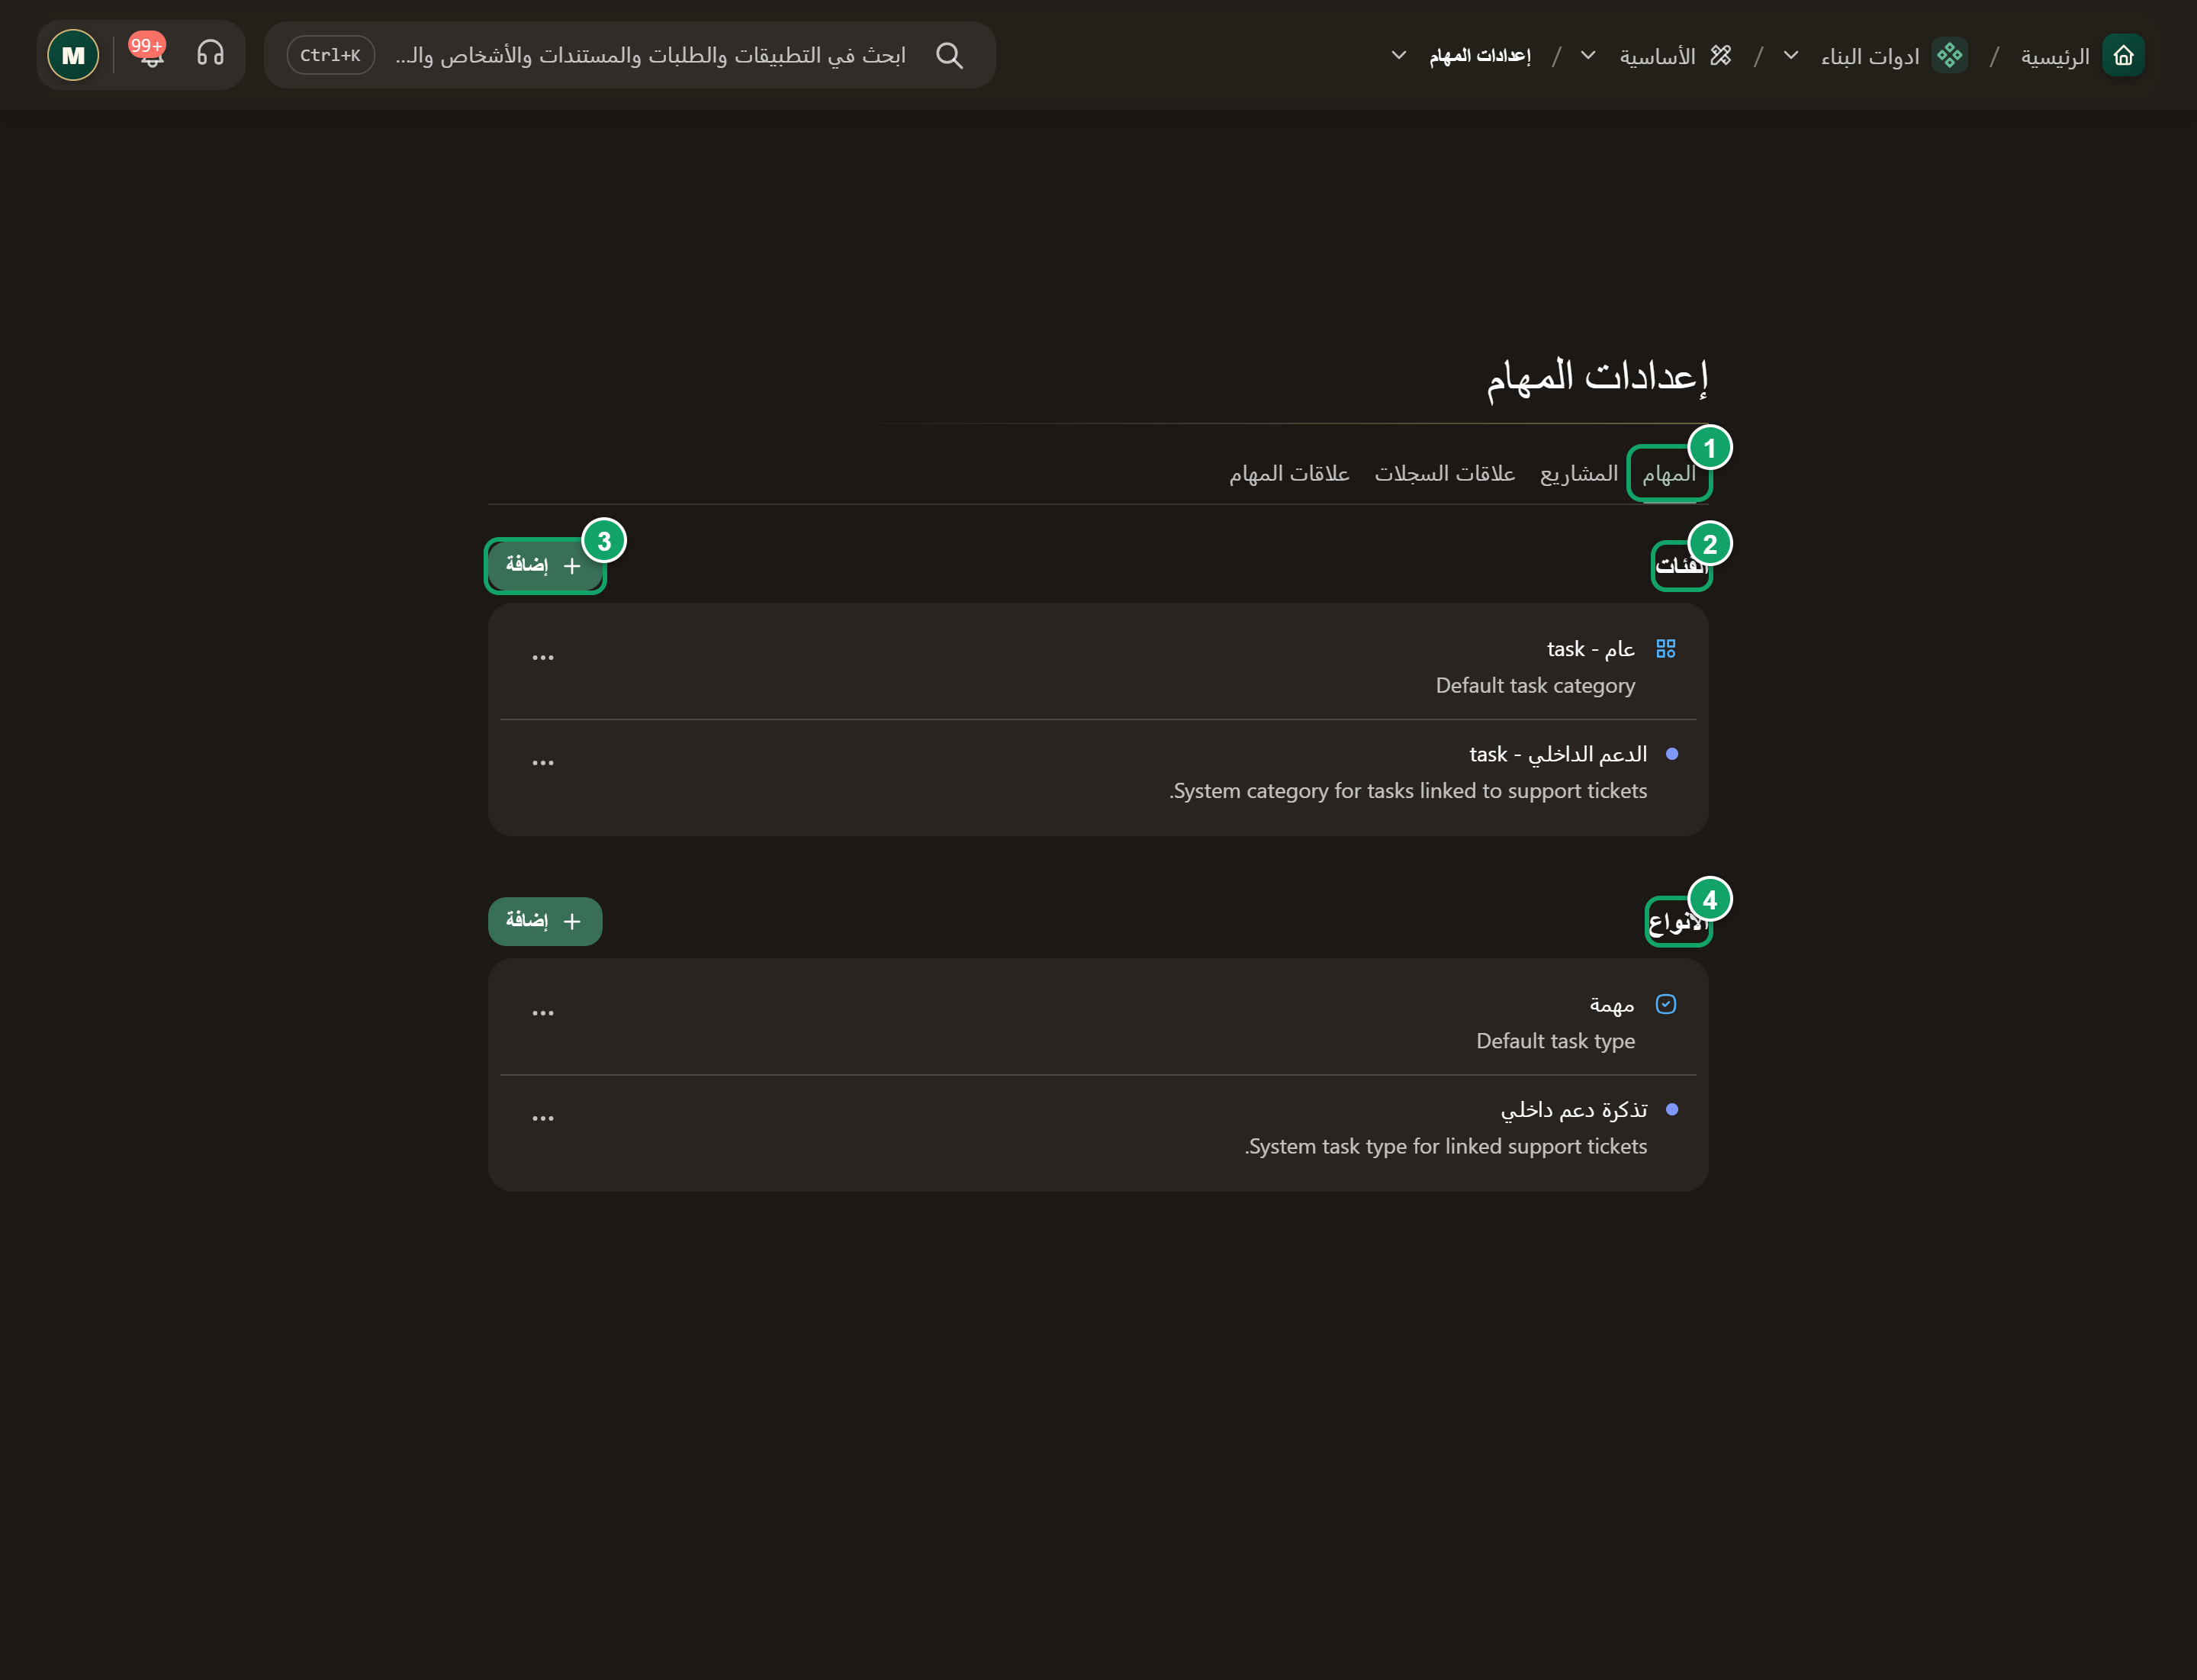
\includegraphics[width=0.95\linewidth,height=0.72\textheight,keepaspectratio]{figures/screens/ch04-settings-ar.png}
\caption{إعدادات أنواع المهام}
\label{fig:tasks-settings-settings}
\shotnote{تقسم «إعدادات المهام» التهيئة إلى أربعة تبويبات: «المهام» و«المشاريع» و«علاقات السجلات» و«علاقات المهام». ويعرض تبويب «المهام» الفئات والأنواع التي يختار منها المستخدم عند إنشاء مهمة، ومنها الفئة والنوع الافتراضيان. ولأن أي تعديل هنا يمس كل مهمة تستخدم النوع، فراجع أثره قبل تغييره. ① تبويب «المهام». ② «الفئات». ③ «إضافة»: ينشئ فئة جديدة. ④ «الأنواع»: تحدد شكل كل مهمة.}
\end{figure}

\begin{figure}[H]
\centering
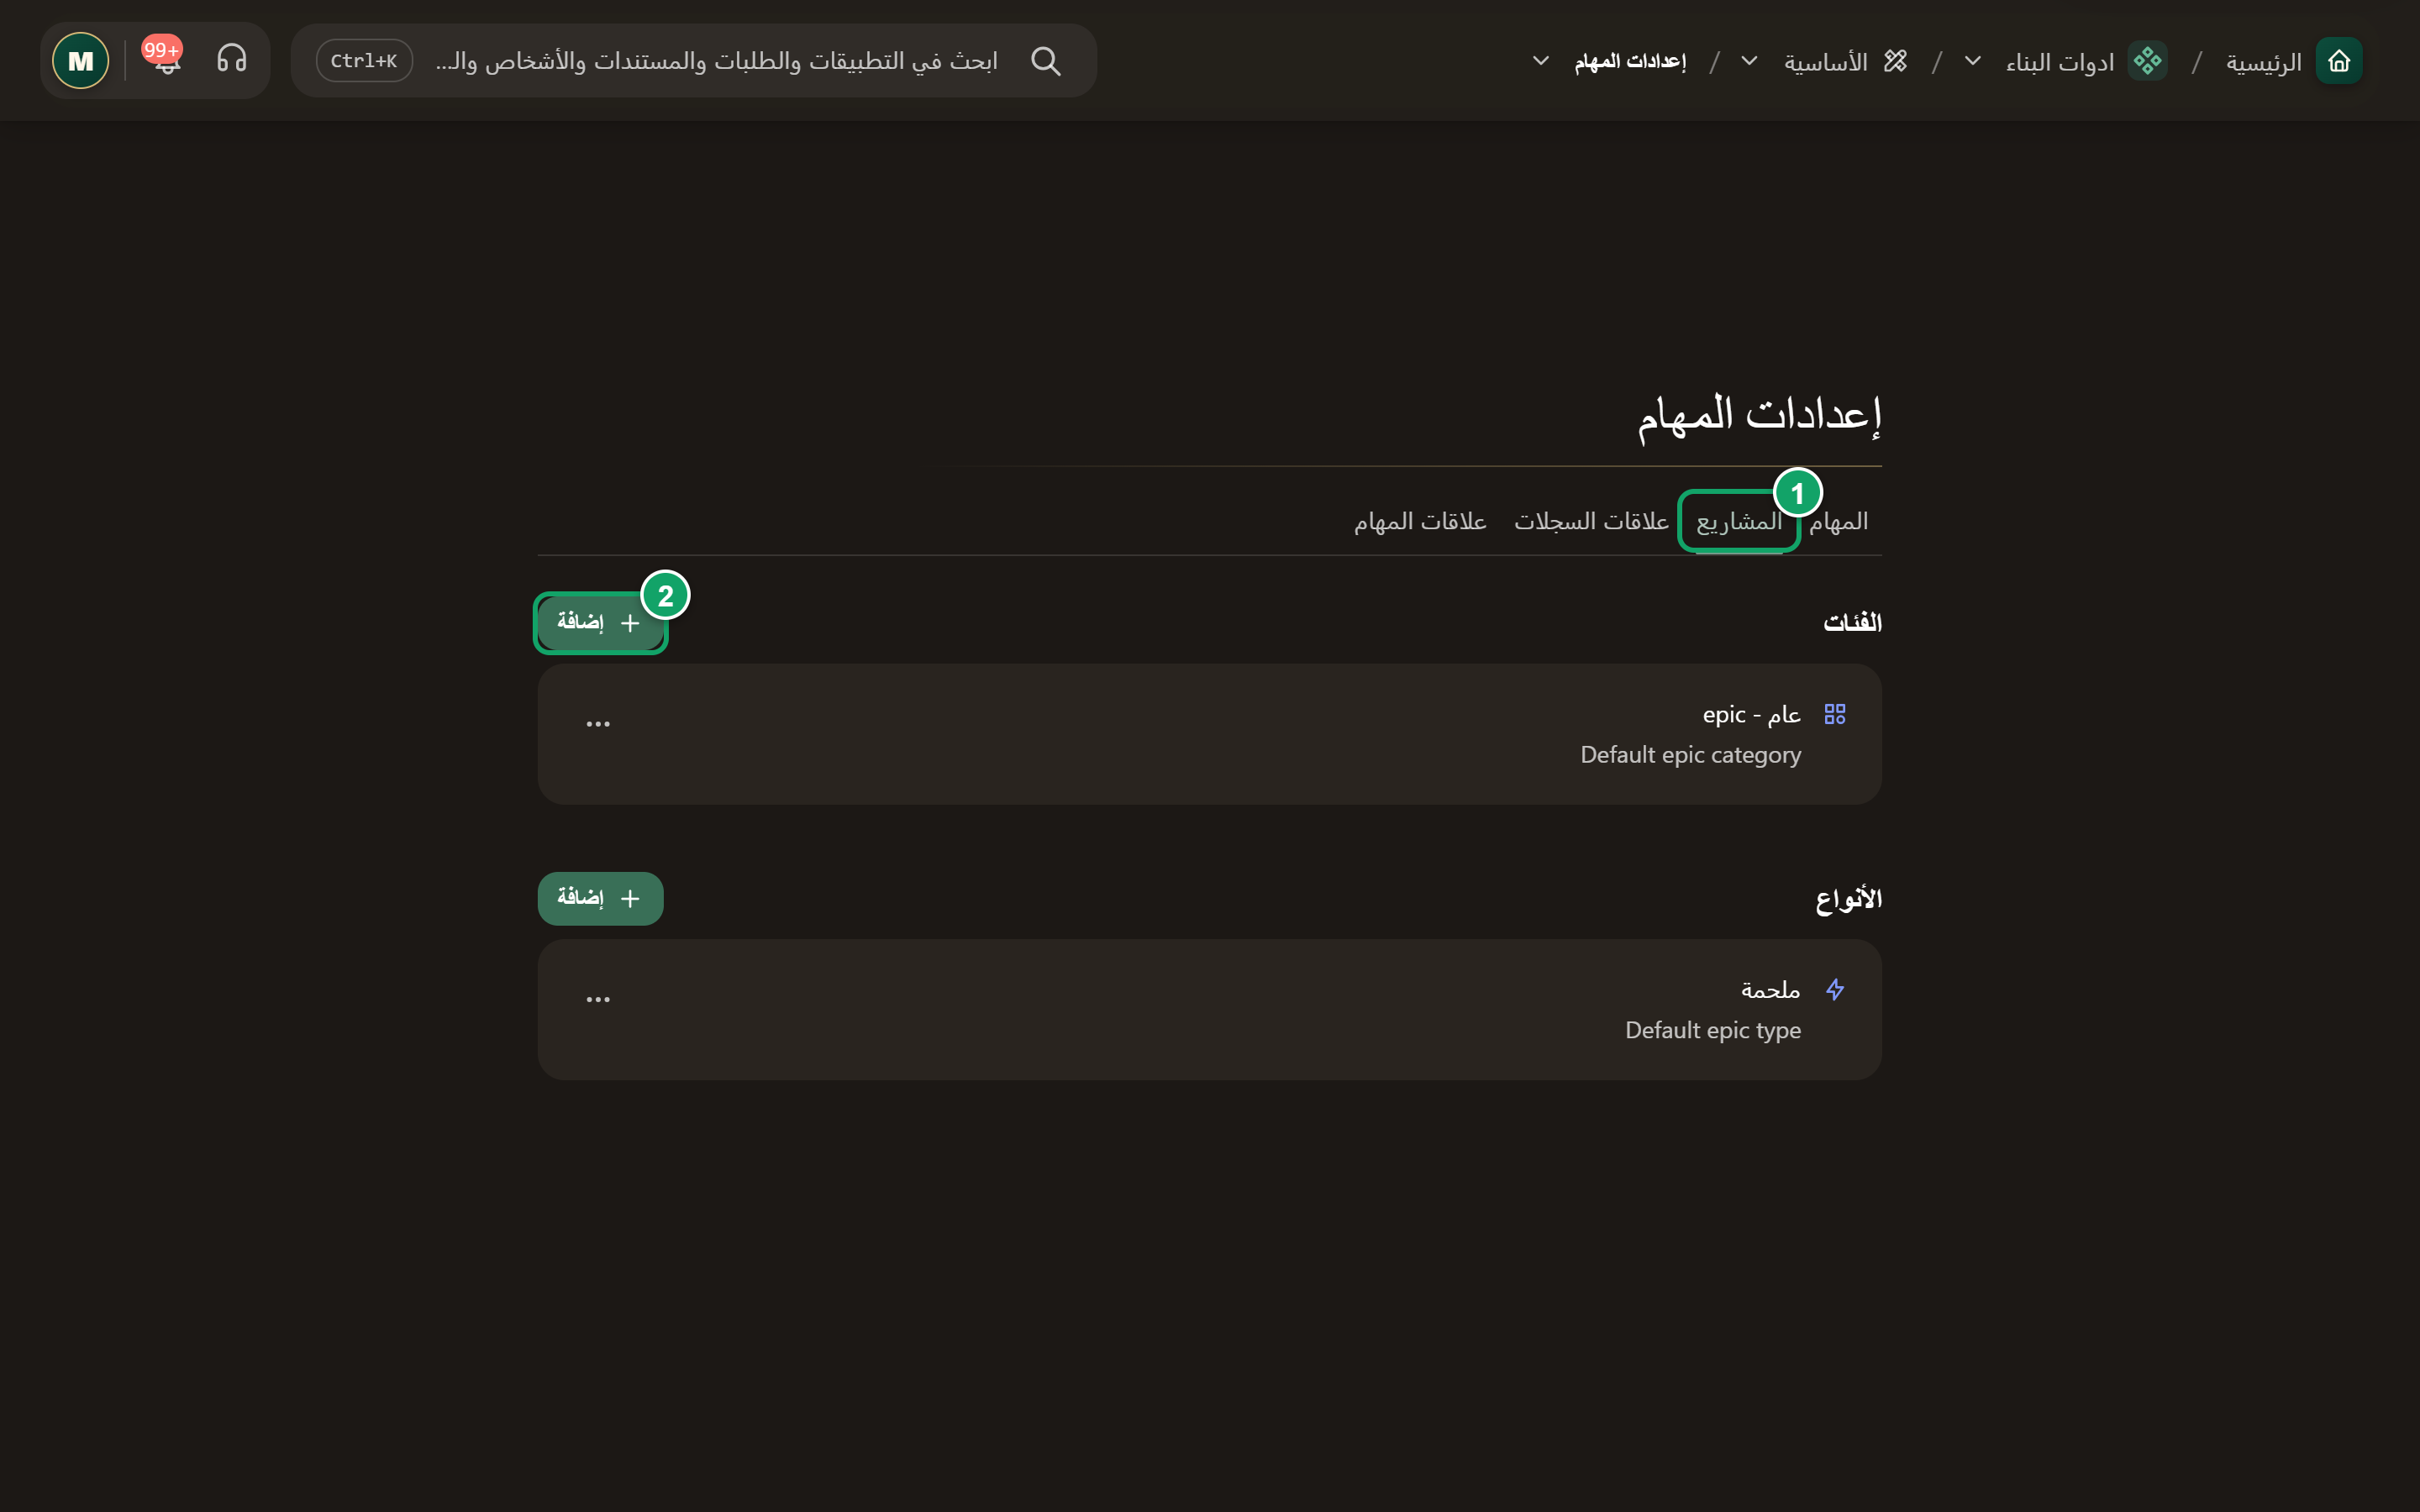
\includegraphics[width=0.95\linewidth,height=0.72\textheight,keepaspectratio]{figures/screens/ch04-settings-epics-ar.png}
\caption{إعدادات المهام الكبرى}
\label{fig:tasks-settings-settings-epics}
\shotnote{يضبط تبويب «المشاريع» هنا فئات المهام الكبرى وأنواعها بمعزل عن فئات المهام العادية، ويظهر في test2 النوع الافتراضي «ملحمة». ولا صلة لهذا التبويب بتطبيق المشاريع والتخطيط رغم تشابه الاسم. ① تبويب «المشاريع». ② «إضافة»: ينشئ إعداداً جديداً للمهام الكبرى.}
\end{figure}

\begin{figure}[H]
\centering
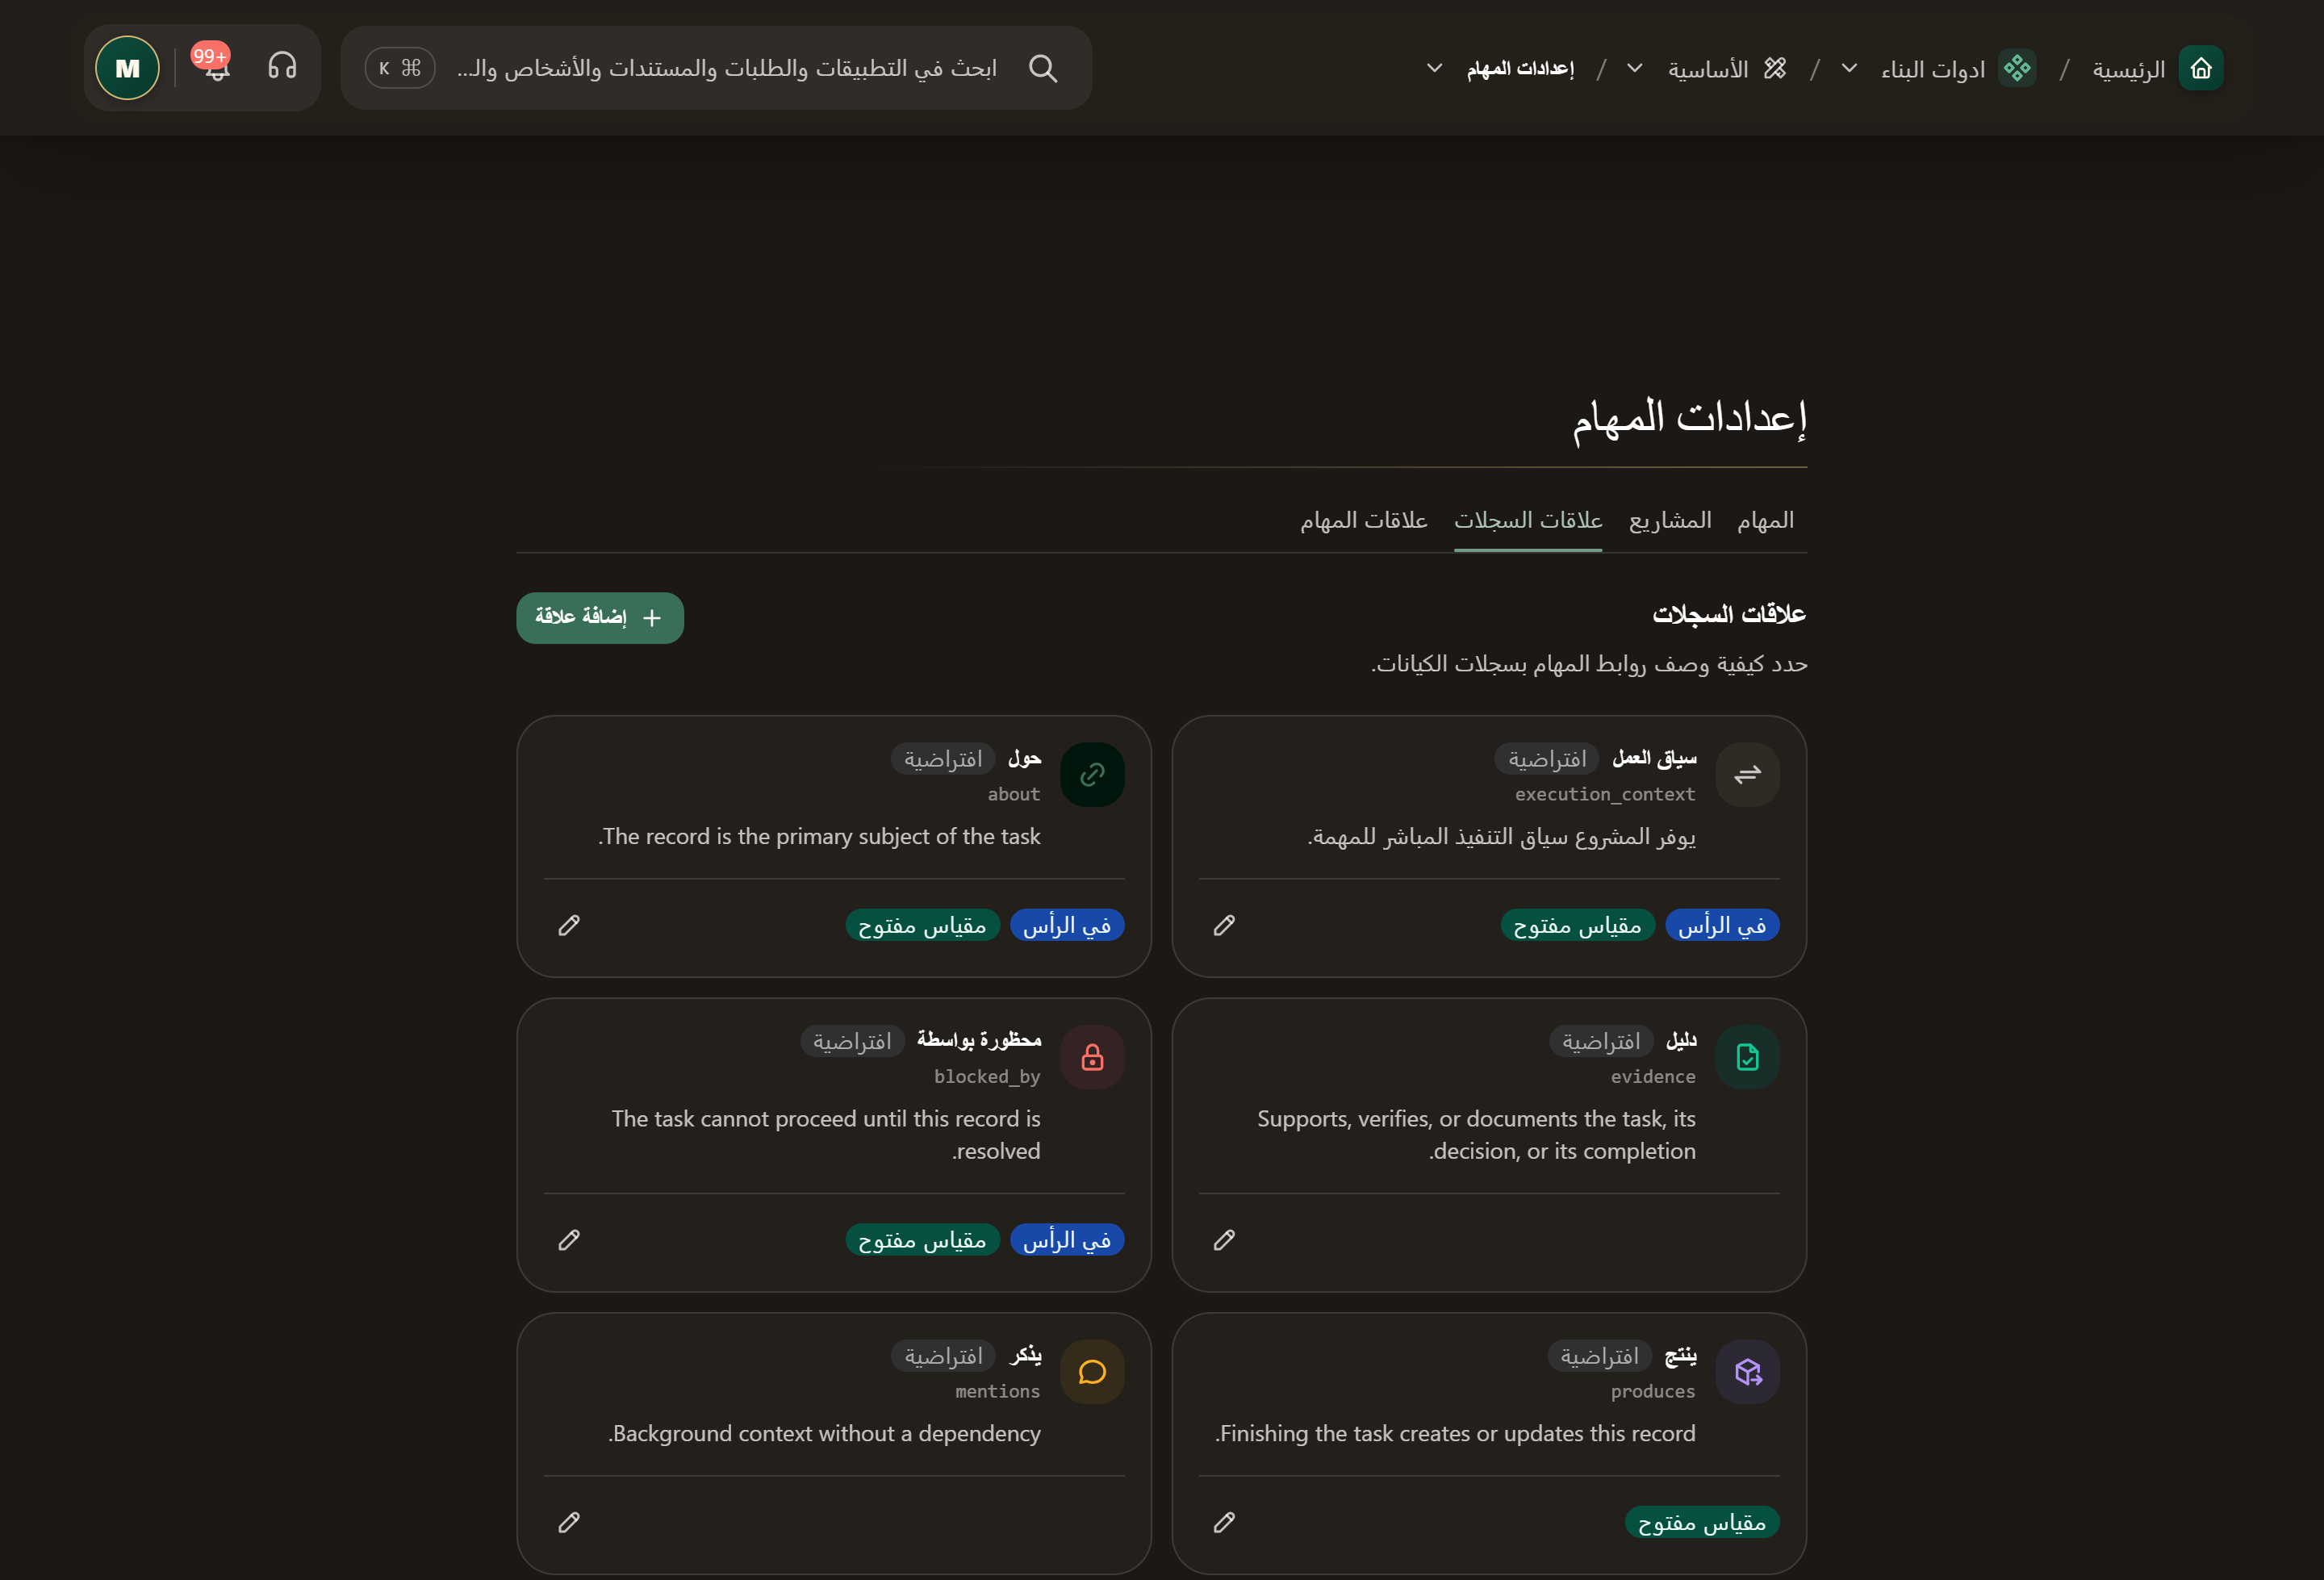
\includegraphics[width=0.95\linewidth,height=0.72\textheight,keepaspectratio]{figures/screens/ch04-settings-records-ar.png}
\caption{إعداد علاقات السجلات}
\label{fig:tasks-settings-settings-records}
\shotnote{يعرّف تبويب «علاقات السجلات» المعاني التي تختار منها عند ربط مهمة بسجل، مثل «دليل» و«ينتج» و«محظورة بواسطة»، ولكل معنى وصف يشرح أثره. وبذلك يفهم الفريق سبب الرابط لا مجرد وجوده. وتظهر هنا الأنواع الافتراضية، ويضيف المسؤول غيرها من «إضافة علاقة». ① تبويب «علاقات السجلات». ② «إضافة علاقة»: ينشئ نوعاً جديداً لربط المهام بالسجلات.}
\end{figure}

\begin{figure}[H]
\centering
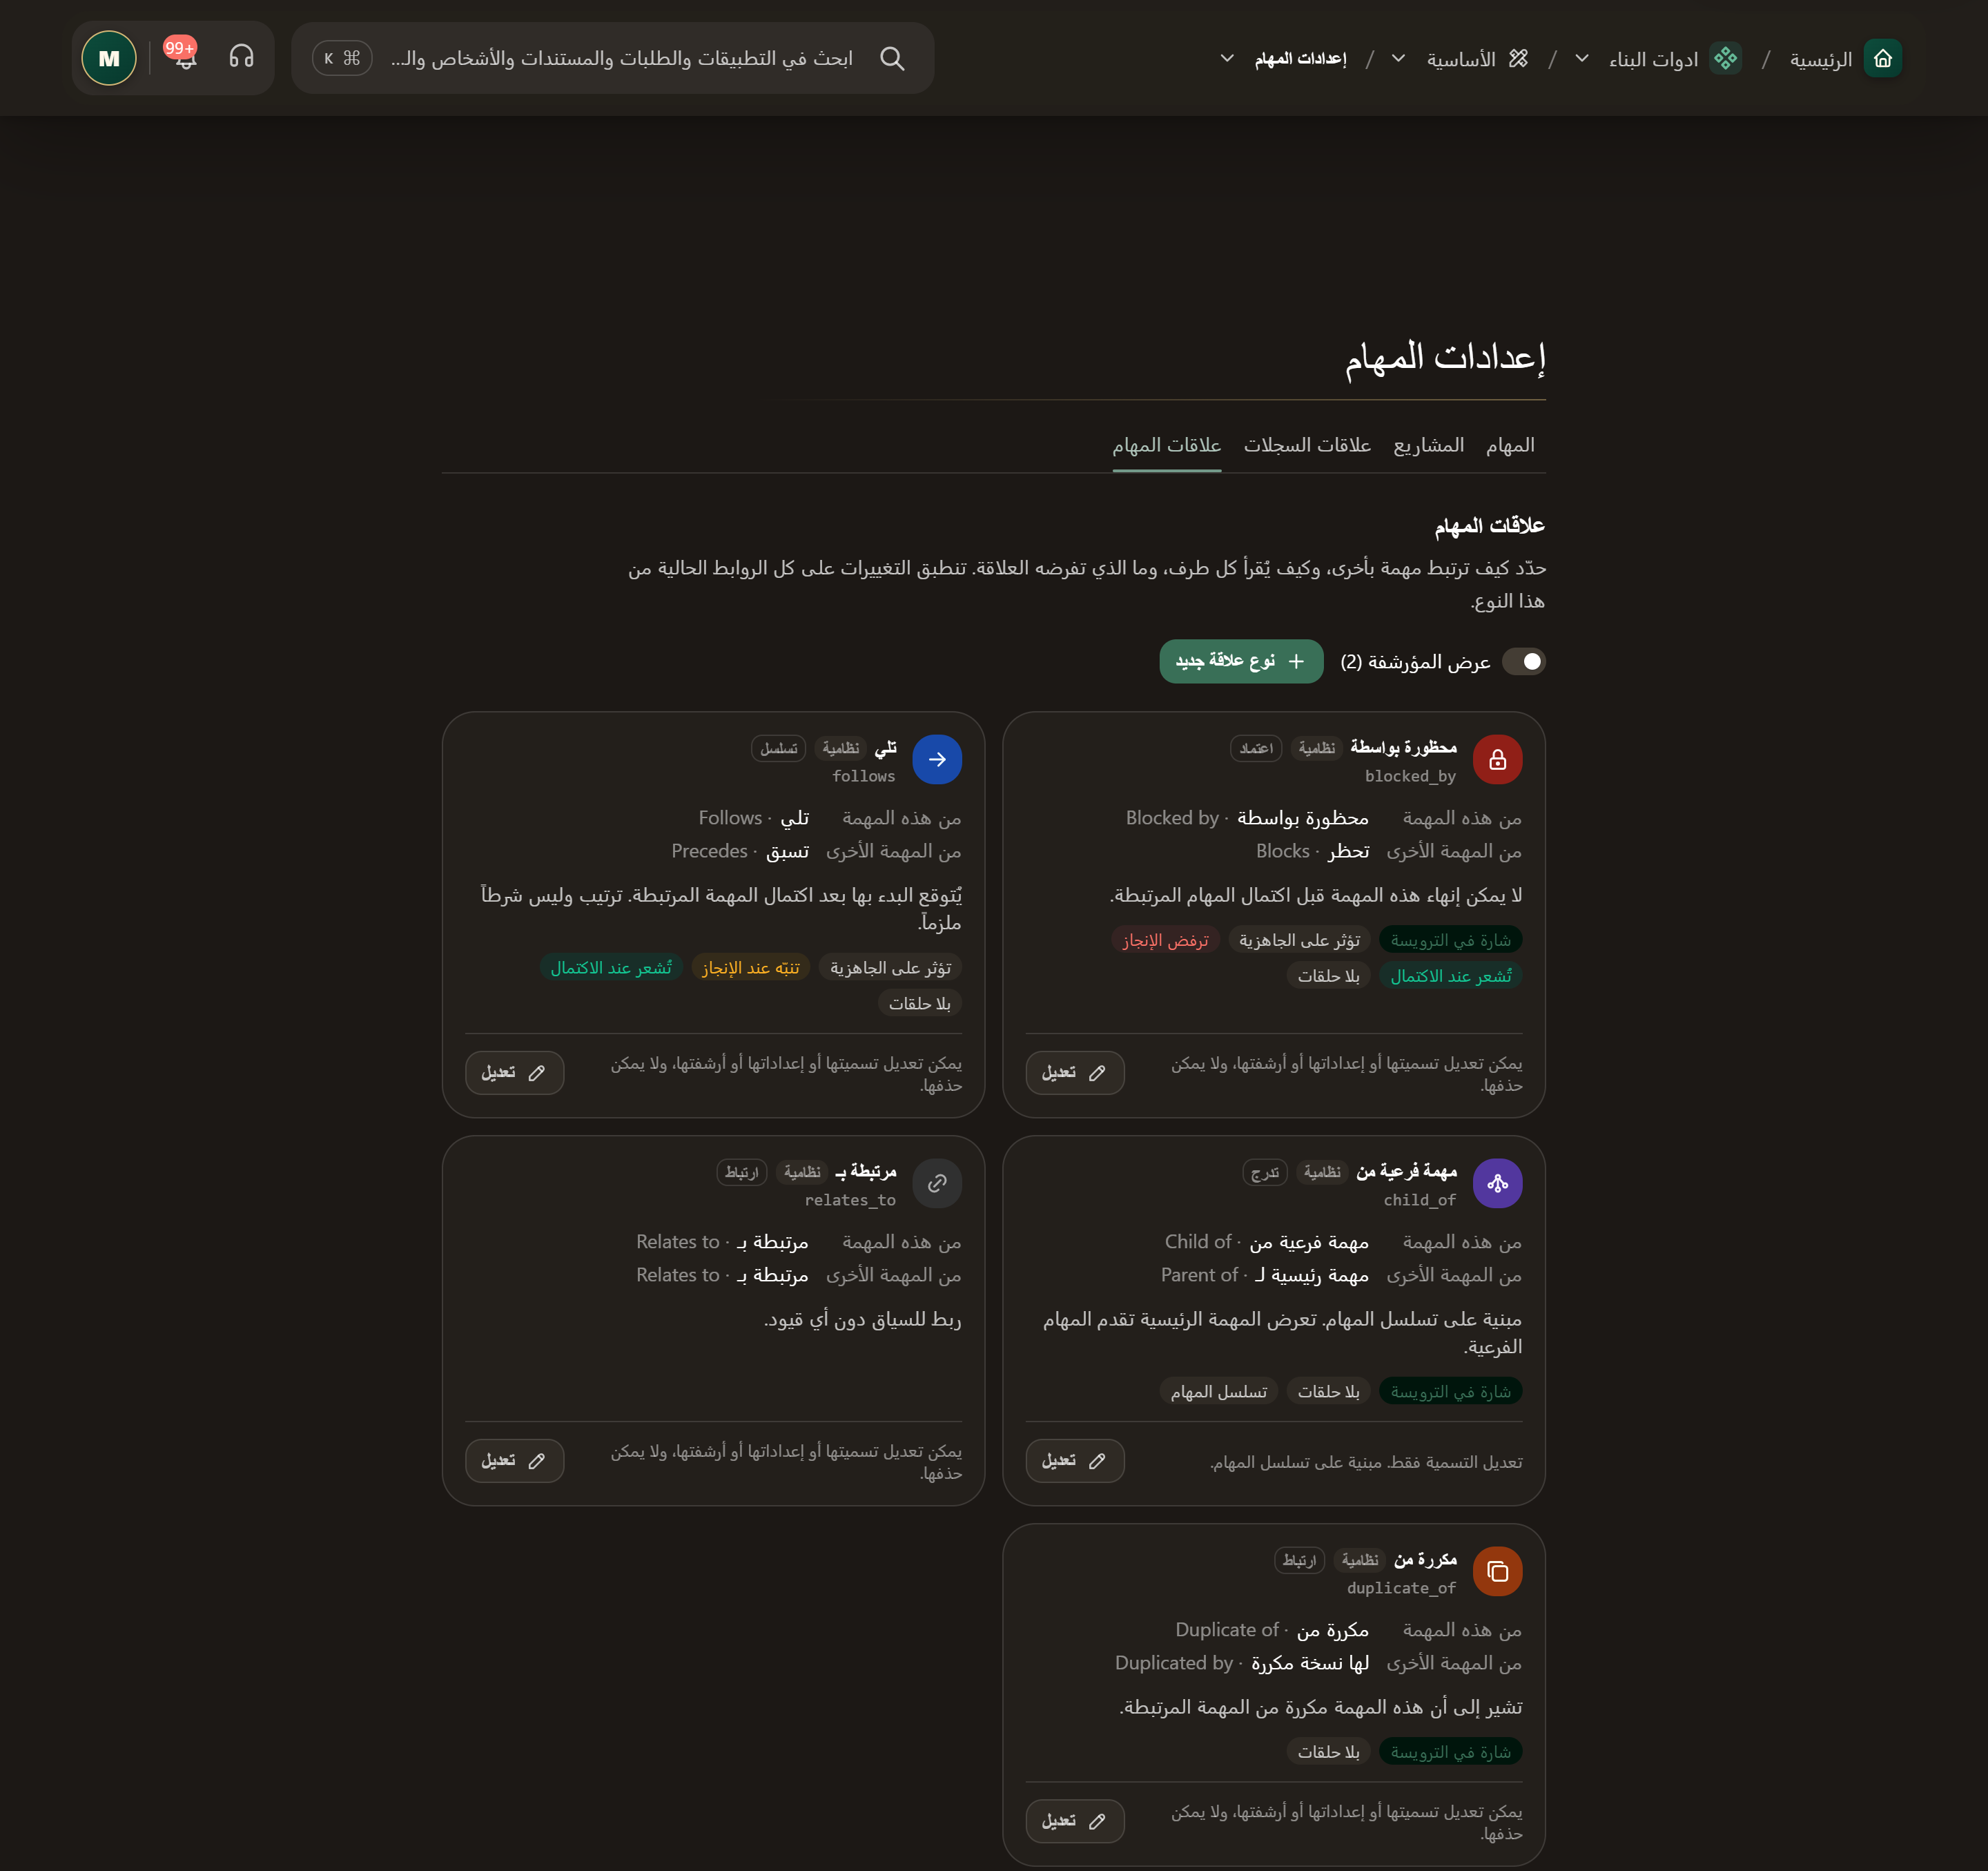
\includegraphics[width=0.95\linewidth,height=0.72\textheight,keepaspectratio]{figures/screens/ch04-settings-relations-ar.png}
\caption{إعداد علاقات المهام}
\label{fig:tasks-settings-settings-relations}
\shotnote{يحدد تبويب «علاقات المهام» كيف ترتبط مهمة بأخرى وكيف تُقرأ العلاقة من كل طرف، مثل «محظورة بواسطة» و«مهمة فرعية من». وتختلف آثارها: فعلاقة الحجب وحدها تحمل هنا شارة «ترفض الإنجاز»، بينما يكتفي غيرها بالترتيب أو الربط. ويمكن تعديل تسمية العلاقات النظامية أو أرشفتها، لكن لا يمكن حذفها. ① تبويب «علاقات المهام». ② «نوع علاقة جديد»: ينشئ نوعاً جديداً لربط المهام بعضها ببعض.}
\end{figure}

\begin{table}[H]
\centering
\caption{ما الذي تجده هنا؟}
\label{tab:tasks-settings-data}
\begin{tabularx}{\linewidth}{R{3.6cm} Y}
\rcHeaderRow
\thh{القسم} & \thh{المحتوى والإجراء}\\
المهام والمهام الكبرى & فئات وأنواع مستقلة لكل منهما، ولكل منها اسم ووصف ولون وأيقونة. ويحدد النوع الفئة وقالب الحالات الافتراضيين ومن يُسمح له باستخدامه.\\
قواعد النوع & العلاقات المطلوبة وحدودها، وإعدادات تحديث التقدم وتواتره بحسب الخيارات المتاحة.\\
علاقات السجلات والمهام & أنواع العلاقات وتسمياتها واتجاهها وقيودها. ميّز العلاقة العادية من العلاقة التي تمنع الإكمال.\\
\end{tabularx}
\end{table}

\begin{figure}[H]
\centering
\begin{tikzpicture}[node distance=0.5cm]
\node[stepBox] (a) {\RL{مراجعة النوع}};
\node[stepBox,below=of a] (b) {\RL{تحديد القواعد}};
\node[stepBox,below=of b] (c) {\RL{اختبار مهمة}};
\draw[flowsTo] (a) -- (b);
\draw[flowsTo] (b) -- (c);
\end{tikzpicture}
\rclegend
\caption{خطوات الاستخدام}
\label{fig:tasks-settings-flow}
\shotnote{يبدأ المخطط من النوع لأن القواعد مرتبطة به: راجع النوع، ثم حدد قواعده، ثم أنشئ مهمة اختبار بهذا النوع. فمهمة الاختبار تكشف أثر الإعداد في الحقول والانتقالات قبل أن يصل إلى عمل الفريق اليومي.}
\end{figure}

\subsection{خطوات العمل والتحقق}
\begin{enumerate}
\item افتح «إعدادات المهام» واختر تبويب «المهام»، أو «المشاريع» للمهام الكبرى، وراجع الفئات والأنواع الحالية قبل الإضافة.
\item افتح النوع، وراجع الاسم والفئة وقالب الحالات والسماح بالاستخدام، ثم راجع قواعد العلاقات والتقدم واحفظ التغييرات بعد اعتمادها.
\item أنشئ مهمة اختبار بهذا النوع في مجموعة مناسبة، وتحقق من ظهور الحقول والقواعد وانتقالات الحالة المتوقعة.
\end{enumerate}

\textbf{تحقق ومعالجة المشكلة:} إذا اختفى نوع من خيارات الإضافة، فراجع قيد المجموعة والسماح باستخدام النوع والصلاحيات. ولا تغيّر إعدادات مشتركة لتتجاوز خطأ في مهمة واحدة.

\clearpage
\section{قوالب الحالات}
\label{sec:tasks-feature-statuses}

يحدد قالب الحالات مراحل العمل والانتقالات بينها. ويُربط القالب بنوع المهمة حتى تسلك المهام مساراً يناسب طبيعة العمل.

\textbf{المسار ومن يستخدمه:} «أدوات البناء» ← «قوالب الحالات». يستخدمها المسؤول عن مسارات العمل.

\begin{rcnote}[مثال: شركة الأفق]
تحتاج مهام زيارات الأفق إلى بدء التنفيذ ثم مراجعة النتيجة، لذلك يراجع المسؤول قالبها مع سارة قبل أن يستخدمه الفريق.
\end{rcnote}

\begin{figure}[H]
\centering
\includegraphics[width=0.95\linewidth,height=0.72\textheight,keepaspectratio]{figures/screens/ch04-statuses-ar.png}
\caption{قائمة قوالب الحالات}
\label{fig:tasks-statuses-statuses}
\shotnote{تعرض «قوالب الحالات» كل القوالب المتاحة في المؤسسة مع إصدار كل قالب، ومنها قوالب تخدم الخطط وغيرها لا المهام وحدها. لذلك حدّد القالب الذي يستخدمه نوع مهمتك قبل أي تعديل؛ فهذه صفحة تهيئة مشتركة، وليست قائمة مهام الموظف. ① عنوان صفحة «قوالب الحالات». ② «إضافة»: ينشئ قالب حالات جديداً.}
\end{figure}

\begin{table}[H]
\centering
\caption{ما الذي تجده هنا؟}
\label{tab:tasks-statuses-data}
\begin{tabularx}{\linewidth}{R{3.6cm} Y}
\rcHeaderRow
\thh{القسم} & \thh{المحتوى والإجراء}\\
القالب والحالات & اسم القالب ومراحله ومعنى كل مرحلة. وتختلف أسماء الحالات بحسب إعداد المؤسسة.\\
الانتقالات & الإجراءات التي تنقل العمل بين المراحل، مع شروطها وصلاحياتها بحسب القالب.\\
الارتباط بالنوع & يختار نوع المهمة قالباً افتراضياً، لذلك راجع النوع بعد تعديل القالب.\\
تنظيم القوالب ونقلها & أنشئ «مجلد جديد» وانقل القوالب إليه، واستورد ملف JSON أو صدّره. وتتيح قائمة القالب التعديل أو الحذف بحسب الصلاحية.\\
\end{tabularx}
\end{table}

\begin{figure}[H]
\centering
\begin{tikzpicture}[node distance=0.5cm]
\node[stepBox] (a) {\RL{تعريف المراحل}};
\node[stepBox,below=of a] (b) {\RL{مراجعة الانتقالات}};
\node[stepBox,below=of b] (c) {\RL{الربط بالنوع والاختبار}};
\draw[flowsTo] (a) -- (b);
\draw[flowsTo] (b) -- (c);
\end{tikzpicture}
\rclegend
\caption{خطوات الاستخدام}
\label{fig:tasks-statuses-flow}
\shotnote{يرتب المخطط بناء المسار: عرّف المراحل أولاً، ثم راجع الانتقالات التي تنقل العمل بينها، وبعدها اربط القالب بالنوع وجرّبه. فلا يظهر أثر القالب في أي مهمة إلا من خلال نوع يستخدمه.}
\end{figure}

\subsection{خطوات العمل والتحقق}
\begin{enumerate}
\item افتح «قوالب الحالات» واختر القالب الذي يستخدمه نوع المهمة، وراجع مراحله وانتقالاته قبل التعديل.
\item راجع كل انتقال: من أي مرحلة يبدأ، وإلى أين يصل، ومن ينفّذه. واحفظ فقط التعديلات المعتمدة في مؤسستك.
\item ارجع إلى نوع المهمة وتحقق من القالب المختار، ثم جرّب المسار على مهمة اختبار.
\end{enumerate}

\textbf{تحقق ومعالجة المشكلة:} إذا غاب إجراء متوقع، فراجع المرحلة الحالية وشروط الانتقال والصلاحية. ولا تجعل تغيير اسم الحالة بديلاً عن تنفيذ الانتقال الصحيح.
